\documentclass[twoside]{book}

% Packages required by doxygen
\usepackage{fixltx2e}
\usepackage{calc}
\usepackage{doxygen}
\usepackage[export]{adjustbox} % also loads graphicx
\usepackage{graphicx}
\usepackage[utf8]{inputenc}
\usepackage{makeidx}
\usepackage{multicol}
\usepackage{multirow}
\PassOptionsToPackage{warn}{textcomp}
\usepackage{textcomp}
\usepackage[nointegrals]{wasysym}
\usepackage[table]{xcolor}

% Font selection
\usepackage[T1]{fontenc}
\usepackage[scaled=.90]{helvet}
\usepackage{courier}
\usepackage{amssymb}
\usepackage{sectsty}
\renewcommand{\familydefault}{\sfdefault}
\allsectionsfont{%
  \fontseries{bc}\selectfont%
  \color{darkgray}%
}
\renewcommand{\DoxyLabelFont}{%
  \fontseries{bc}\selectfont%
  \color{darkgray}%
}
\newcommand{\+}{\discretionary{\mbox{\scriptsize$\hookleftarrow$}}{}{}}

% Page & text layout
\usepackage{geometry}
\geometry{%
  a4paper,%
  top=2.5cm,%
  bottom=2.5cm,%
  left=2.5cm,%
  right=2.5cm%
}
\tolerance=750
\hfuzz=15pt
\hbadness=750
\setlength{\emergencystretch}{15pt}
\setlength{\parindent}{0cm}
\setlength{\parskip}{3ex plus 2ex minus 2ex}
\makeatletter
\renewcommand{\paragraph}{%
  \@startsection{paragraph}{4}{0ex}{-1.0ex}{1.0ex}{%
    \normalfont\normalsize\bfseries\SS@parafont%
  }%
}
\renewcommand{\subparagraph}{%
  \@startsection{subparagraph}{5}{0ex}{-1.0ex}{1.0ex}{%
    \normalfont\normalsize\bfseries\SS@subparafont%
  }%
}
\makeatother

% Headers & footers
\usepackage{fancyhdr}
\pagestyle{fancyplain}
\fancyhead[LE]{\fancyplain{}{\bfseries\thepage}}
\fancyhead[CE]{\fancyplain{}{}}
\fancyhead[RE]{\fancyplain{}{\bfseries\leftmark}}
\fancyhead[LO]{\fancyplain{}{\bfseries\rightmark}}
\fancyhead[CO]{\fancyplain{}{}}
\fancyhead[RO]{\fancyplain{}{\bfseries\thepage}}
\fancyfoot[LE]{\fancyplain{}{}}
\fancyfoot[CE]{\fancyplain{}{}}
\fancyfoot[RE]{\fancyplain{}{\bfseries\scriptsize Generated by Doxygen }}
\fancyfoot[LO]{\fancyplain{}{\bfseries\scriptsize Generated by Doxygen }}
\fancyfoot[CO]{\fancyplain{}{}}
\fancyfoot[RO]{\fancyplain{}{}}
\renewcommand{\footrulewidth}{0.4pt}
\renewcommand{\chaptermark}[1]{%
  \markboth{#1}{}%
}
\renewcommand{\sectionmark}[1]{%
  \markright{\thesection\ #1}%
}

% Indices & bibliography
\usepackage{natbib}
\usepackage[titles]{tocloft}
\setcounter{tocdepth}{3}
\setcounter{secnumdepth}{5}
\makeindex

% Hyperlinks (required, but should be loaded last)
\usepackage{ifpdf}
\ifpdf
  \usepackage[pdftex,pagebackref=true]{hyperref}
\else
  \usepackage[ps2pdf,pagebackref=true]{hyperref}
\fi
\hypersetup{%
  colorlinks=true,%
  linkcolor=blue,%
  citecolor=blue,%
  unicode%
}

% Custom commands
\newcommand{\clearemptydoublepage}{%
  \newpage{\pagestyle{empty}\cleardoublepage}%
}

\usepackage{caption}
\captionsetup{labelsep=space,justification=centering,font={bf},singlelinecheck=off,skip=4pt,position=top}

%===== C O N T E N T S =====

\begin{document}

% Titlepage & ToC
\hypersetup{pageanchor=false,
             bookmarksnumbered=true,
             pdfencoding=unicode
            }
\pagenumbering{alph}
\begin{titlepage}
\vspace*{7cm}
\begin{center}%
{\Large Py\+C\+UB\+: Machine exploration of the Codon Usage Bias }\\
\vspace*{1cm}
{\large Generated by Doxygen 1.8.14}\\
\end{center}
\end{titlepage}
\clearemptydoublepage
\pagenumbering{roman}
\tableofcontents
\clearemptydoublepage
\pagenumbering{arabic}
\hypersetup{pageanchor=true}

%--- Begin generated contents ---
\chapter{Namespace Index}
\section{Packages}
Here are the packages with brief descriptions (if available)\+:\begin{DoxyCompactList}
\item\contentsline{section}{\mbox{\hyperlink{namespace_py_c_u_b}{Py\+C\+UB}} \\*Main object of the project that allows the user to access most of the functions }{\pageref{namespace_py_c_u_b}}{}
\end{DoxyCompactList}

\chapter{Hierarchical Index}
\section{Class Hierarchy}
This inheritance list is sorted roughly, but not completely, alphabetically\+:\begin{DoxyCompactList}
\item dict\begin{DoxyCompactList}
\item \contentsline{section}{Py\+C\+U\+B.\+utils.\+dotdict}{\pageref{class_py_c_u_b_1_1utils_1_1dotdict}}{}
\end{DoxyCompactList}
\item Mutable\+Mapping\begin{DoxyCompactList}
\item \contentsline{section}{Py\+C\+U\+B.\+homoset.\+Homo\+Set}{\pageref{class_py_c_u_b_1_1homoset_1_1_homo_set}}{}
\end{DoxyCompactList}
\item object\begin{DoxyCompactList}
\item \contentsline{section}{Py\+C\+U\+B.\+espece.\+Espece}{\pageref{class_py_c_u_b_1_1espece_1_1_espece}}{}
\item \contentsline{section}{Py\+C\+U\+B.\+homology.\+homology}{\pageref{class_py_c_u_b_1_1homology_1_1homology}}{}
\item \contentsline{section}{Py\+C\+U\+B.\+py\+C\+U\+B.\+Py\+C\+UB}{\pageref{class_py_c_u_b_1_1py_c_u_b_1_1_py_c_u_b}}{}
\end{DoxyCompactList}
\end{DoxyCompactList}

\chapter{Class Index}
\section{Class List}
Here are the classes, structs, unions and interfaces with brief descriptions\+:\begin{DoxyCompactList}
\item\contentsline{section}{\mbox{\hyperlink{class_py_c_u_b_1_1utils_1_1dotdict}{Py\+C\+U\+B.\+utils.\+dotdict}} \\*Dot.\+notation access to dictionary attributes }{\pageref{class_py_c_u_b_1_1utils_1_1dotdict}}{}
\item\contentsline{section}{\mbox{\hyperlink{class_py_c_u_b_1_1espece_1_1_espece}{Py\+C\+U\+B.\+espece.\+Espece}} \\*Docstring for \mbox{\hyperlink{class_py_c_u_b_1_1espece_1_1_espece}{Espece}} }{\pageref{class_py_c_u_b_1_1espece_1_1_espece}}{}
\item\contentsline{section}{\mbox{\hyperlink{class_py_c_u_b_1_1homology_1_1homology}{Py\+C\+U\+B.\+homology.\+homology}} \\*In homology we store an homology with all its related data, }{\pageref{class_py_c_u_b_1_1homology_1_1homology}}{}
\item\contentsline{section}{\mbox{\hyperlink{class_py_c_u_b_1_1homoset_1_1_homo_set}{Py\+C\+U\+B.\+homoset.\+Homo\+Set}} \\*\mbox{\hyperlink{class_py_c_u_b_1_1homoset_1_1_homo_set}{Homo\+Set}} is the object containing evrey homology as a dictionnary according to thie rhomology code }{\pageref{class_py_c_u_b_1_1homoset_1_1_homo_set}}{}
\item\contentsline{section}{\mbox{\hyperlink{class_py_c_u_b_1_1py_c_u_b_1_1_py_c_u_b}{Py\+C\+U\+B.\+py\+C\+U\+B.\+Py\+C\+UB}} \\*\mbox{\hyperlink{class_py_c_u_b_1_1py_c_u_b_1_1_py_c_u_b}{Py\+C\+UB}} is the main object of the project that allows the user to access most of the functions }{\pageref{class_py_c_u_b_1_1py_c_u_b_1_1_py_c_u_b}}{}
\end{DoxyCompactList}

\chapter{File Index}
\section{File List}
Here is a list of all documented files with brief descriptions\+:\begin{DoxyCompactList}
\item\contentsline{section}{Py\+C\+U\+B/\mbox{\hyperlink{utils_8py}{utils.\+py}} \\*Utils is where utilitary functions are stored (in particular preprocessing functions here) }{\pageref{utils_8py}}{}
\end{DoxyCompactList}

\chapter{Namespace Documentation}
\hypertarget{namespacepy_c_u_b}{}\section{py\+C\+UB Namespace Reference}
\label{namespacepy_c_u_b}\index{py\+C\+UB@{py\+C\+UB}}


" Created by Jeremie K\+A\+L\+F\+ON Date 21 F\+EV 2018 University of Kent, E\+CE paris jkobject.\+com  




\subsection{Detailed Description}
" Created by Jeremie K\+A\+L\+F\+ON Date 21 F\+EV 2018 University of Kent, E\+CE paris jkobject.\+com 
\hypertarget{namespace_py_c_u_b}{}\section{Py\+C\+UB Namespace Reference}
\label{namespace_py_c_u_b}\index{Py\+C\+UB@{Py\+C\+UB}}


is the main object of the project that allows the user to access most of the functions  




\subsection{Detailed Description}
is the main object of the project that allows the user to access most of the functions 

When using it, please follow the documentation and examples on notebooks thought you can still use it as you please and use some of the nice tricks provided here and in python 
\chapter{Class Documentation}
\hypertarget{class_py_c_u_b_1_1espece_1_1_espece}{}\section{Py\+C\+U\+B.\+espece.\+Espece Class Reference}
\label{class_py_c_u_b_1_1espece_1_1_espece}\index{Py\+C\+U\+B.\+espece.\+Espece@{Py\+C\+U\+B.\+espece.\+Espece}}


docstring for \mbox{\hyperlink{class_py_c_u_b_1_1espece_1_1_espece}{Espece}}  


Inheritance diagram for Py\+C\+U\+B.\+espece.\+Espece\+:\begin{figure}[H]
\begin{center}
\leavevmode
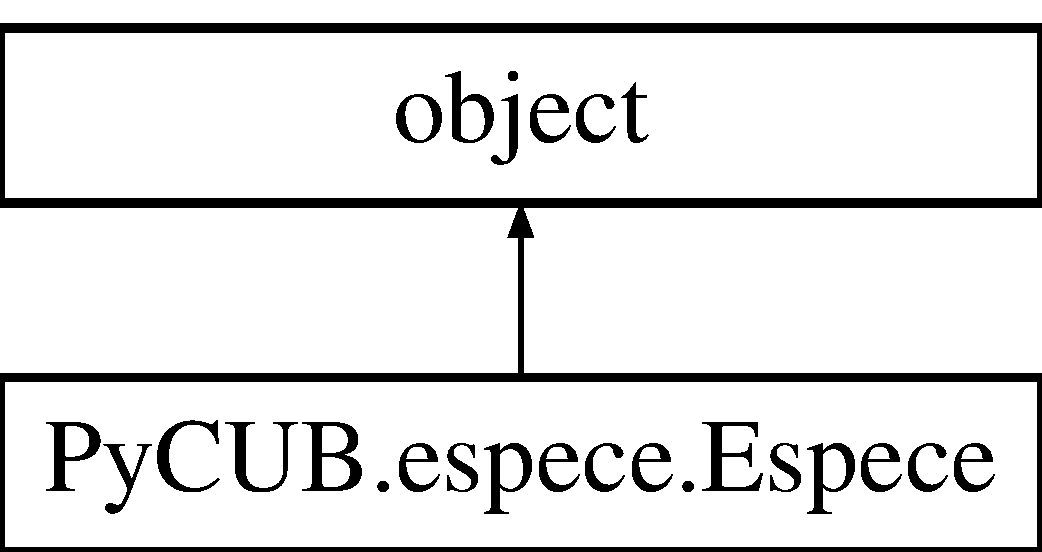
\includegraphics[height=2.000000cm]{class_py_c_u_b_1_1espece_1_1_espece}
\end{center}
\end{figure}
\subsection*{Public Member Functions}
\begin{DoxyCompactItemize}
\item 
\mbox{\Hypertarget{class_py_c_u_b_1_1espece_1_1_espece_a13a7403216d2c03d6e9ec81d6034196e}\label{class_py_c_u_b_1_1espece_1_1_espece_a13a7403216d2c03d6e9ec81d6034196e}} 
def \mbox{\hyperlink{class_py_c_u_b_1_1espece_1_1_espece_a13a7403216d2c03d6e9ec81d6034196e}{\+\_\+\+\_\+init\+\_\+\+\_\+}} (self, kwargs)
\begin{DoxyCompactList}\small\item\em can intialize the file from kwargs as a raw dictionnary for json format (output of dictify) or from regular args. \end{DoxyCompactList}\item 
\mbox{\Hypertarget{class_py_c_u_b_1_1espece_1_1_espece_a4222c359e63e76ea34631a427b62fd60}\label{class_py_c_u_b_1_1espece_1_1_espece_a4222c359e63e76ea34631a427b62fd60}} 
def \mbox{\hyperlink{class_py_c_u_b_1_1espece_1_1_espece_a4222c359e63e76ea34631a427b62fd60}{\+\_\+\+\_\+str\+\_\+\+\_\+}} (self)
\begin{DoxyCompactList}\small\item\em will present some interesting info about this species. \end{DoxyCompactList}\item 
def \mbox{\hyperlink{class_py_c_u_b_1_1espece_1_1_espece_afa35655bb969cbc02456aa74228a1b8d}{get\+\_\+t\+R\+N\+Acopy}} (self, by=\char`\"{}entropy\char`\"{}, setnans=False, kingdom=\textquotesingle{}fungi\textquotesingle{}, base\+C\+Nvalue=2)
\begin{DoxyCompactList}\small\item\em Retrieves t\+R\+NA copy numbers from ensembl DB. \end{DoxyCompactList}\item 
def \mbox{\hyperlink{class_py_c_u_b_1_1espece_1_1_espece_af716fcd7e7e34e12cd7786469d695422}{gettaxons}} (self, kingdom=\textquotesingle{}fungi\textquotesingle{})
\begin{DoxyCompactList}\small\item\em Pars the ensemblgenomes R\+E\+ST A\+PI to retrieve the taxons id. \end{DoxyCompactList}\item 
\mbox{\Hypertarget{class_py_c_u_b_1_1espece_1_1_espece_aed93f9be40c4521c6aed536125268432}\label{class_py_c_u_b_1_1espece_1_1_espece_aed93f9be40c4521c6aed536125268432}} 
def \mbox{\hyperlink{class_py_c_u_b_1_1espece_1_1_espece_aed93f9be40c4521c6aed536125268432}{get\+\_\+epigenomes}} (self)
\begin{DoxyCompactList}\small\item\em get from ensembl all the data about the epigenome that could help asking interesting questions about the C\+UB \end{DoxyCompactList}\end{DoxyCompactItemize}
\subsection*{Public Attributes}
\begin{DoxyCompactItemize}
\item 
\mbox{\Hypertarget{class_py_c_u_b_1_1espece_1_1_espece_a3a33da4c7b0c9163b8673166b306226c}\label{class_py_c_u_b_1_1espece_1_1_espece_a3a33da4c7b0c9163b8673166b306226c}} 
{\bfseries name}
\item 
\mbox{\Hypertarget{class_py_c_u_b_1_1espece_1_1_espece_ae98c1d182e761e4c09a10f8a9994124e}\label{class_py_c_u_b_1_1espece_1_1_espece_ae98c1d182e761e4c09a10f8a9994124e}} 
{\bfseries metadata}
\item 
\mbox{\Hypertarget{class_py_c_u_b_1_1espece_1_1_espece_afbc7dbe8f3dc1f035837bb2ed610f246}\label{class_py_c_u_b_1_1espece_1_1_espece_afbc7dbe8f3dc1f035837bb2ed610f246}} 
{\bfseries is\+\_\+stored}
\item 
\mbox{\Hypertarget{class_py_c_u_b_1_1espece_1_1_espece_adb2006eee970b43f6abe9554690cb424}\label{class_py_c_u_b_1_1espece_1_1_espece_adb2006eee970b43f6abe9554690cb424}} 
{\bfseries num\+\_\+genes}
\item 
\mbox{\Hypertarget{class_py_c_u_b_1_1espece_1_1_espece_ad40242dc0031d44de4c363bd716489e2}\label{class_py_c_u_b_1_1espece_1_1_espece_ad40242dc0031d44de4c363bd716489e2}} 
{\bfseries genome\+\_\+size}
\end{DoxyCompactItemize}
\subsection*{Static Public Attributes}
\begin{DoxyCompactItemize}
\item 
\mbox{\Hypertarget{class_py_c_u_b_1_1espece_1_1_espece_a143141fe25ea32dc24abd314a0f5fdbd}\label{class_py_c_u_b_1_1espece_1_1_espece_a143141fe25ea32dc24abd314a0f5fdbd}} 
{\bfseries code} = None
\item 
\mbox{\Hypertarget{class_py_c_u_b_1_1espece_1_1_espece_ac3d8e577f2e9a0fe6853d51c4bec238d}\label{class_py_c_u_b_1_1espece_1_1_espece_ac3d8e577f2e9a0fe6853d51c4bec238d}} 
int {\bfseries num\+\_\+genes} = 0
\item 
\mbox{\Hypertarget{class_py_c_u_b_1_1espece_1_1_espece_a87ca67e0c2e560e88b72a8bdba456756}\label{class_py_c_u_b_1_1espece_1_1_espece_a87ca67e0c2e560e88b72a8bdba456756}} 
int {\bfseries genome\+\_\+size} = 0
\item 
\mbox{\Hypertarget{class_py_c_u_b_1_1espece_1_1_espece_ae066a956b3f9f29d676162fbf9773a0f}\label{class_py_c_u_b_1_1espece_1_1_espece_ae066a956b3f9f29d676162fbf9773a0f}} 
{\bfseries link} = None
\item 
dictionary {\bfseries metadata}
\item 
\mbox{\Hypertarget{class_py_c_u_b_1_1espece_1_1_espece_a8befee83c9b6ecfc8b07e66b6251afa4}\label{class_py_c_u_b_1_1espece_1_1_espece_a8befee83c9b6ecfc8b07e66b6251afa4}} 
bool {\bfseries is\+\_\+stored} = False
\item 
\mbox{\Hypertarget{class_py_c_u_b_1_1espece_1_1_espece_accf54132a0346377a2cf7a461a129dc1}\label{class_py_c_u_b_1_1espece_1_1_espece_accf54132a0346377a2cf7a461a129dc1}} 
string {\bfseries name} = \textquotesingle{}\textquotesingle{}
\item 
\mbox{\Hypertarget{class_py_c_u_b_1_1espece_1_1_espece_aae7cf0e3c6f359bd2970006817e80ed3}\label{class_py_c_u_b_1_1espece_1_1_espece_aae7cf0e3c6f359bd2970006817e80ed3}} 
{\bfseries taxonid} = None
\item 
\mbox{\Hypertarget{class_py_c_u_b_1_1espece_1_1_espece_a89cd4e211bf028a4d141202e8a885b58}\label{class_py_c_u_b_1_1espece_1_1_espece_a89cd4e211bf028a4d141202e8a885b58}} 
{\bfseries copynumbers} = None
\item 
\mbox{\Hypertarget{class_py_c_u_b_1_1espece_1_1_espece_a2dc4b3f0d2006aac69a9846ba834d209}\label{class_py_c_u_b_1_1espece_1_1_espece_a2dc4b3f0d2006aac69a9846ba834d209}} 
{\bfseries average\+\_\+entropy} = None
\item 
\mbox{\Hypertarget{class_py_c_u_b_1_1espece_1_1_espece_a2991e13a2c75e2e899f3f8f773d1d9b6}\label{class_py_c_u_b_1_1espece_1_1_espece_a2991e13a2c75e2e899f3f8f773d1d9b6}} 
{\bfseries average\+\_\+size} = None
\item 
\mbox{\Hypertarget{class_py_c_u_b_1_1espece_1_1_espece_ac7ce087a6722a531555c005c6b37ae88}\label{class_py_c_u_b_1_1espece_1_1_espece_ac7ce087a6722a531555c005c6b37ae88}} 
{\bfseries var\+\_\+entropy} = None
\item 
\mbox{\Hypertarget{class_py_c_u_b_1_1espece_1_1_espece_a27d1e4719b819c4e99e889904fbff5ed}\label{class_py_c_u_b_1_1espece_1_1_espece_a27d1e4719b819c4e99e889904fbff5ed}} 
{\bfseries fullentropy} = None
\item 
\mbox{\Hypertarget{class_py_c_u_b_1_1espece_1_1_espece_a7c21598e68d19819e523bb08af5a815d}\label{class_py_c_u_b_1_1espece_1_1_espece_a7c21598e68d19819e523bb08af5a815d}} 
{\bfseries fullvarentropy} = None
\item 
\mbox{\Hypertarget{class_py_c_u_b_1_1espece_1_1_espece_a4c199498e2938fdd8521fb724e9f4e58}\label{class_py_c_u_b_1_1espece_1_1_espece_a4c199498e2938fdd8521fb724e9f4e58}} 
{\bfseries full\+G\+Ccount} = None
\item 
\mbox{\Hypertarget{class_py_c_u_b_1_1espece_1_1_espece_a6f99cfcc3643e72bf48a2479c81b7e03}\label{class_py_c_u_b_1_1espece_1_1_espece_a6f99cfcc3643e72bf48a2479c81b7e03}} 
{\bfseries var\+G\+Ccount} = None
\item 
\mbox{\Hypertarget{class_py_c_u_b_1_1espece_1_1_espece_a32834ad6a3a42b850438789ae1e7270b}\label{class_py_c_u_b_1_1espece_1_1_espece_a32834ad6a3a42b850438789ae1e7270b}} 
{\bfseries mean\+G\+Chomo} = None
\item 
\mbox{\Hypertarget{class_py_c_u_b_1_1espece_1_1_espece_a5fdd0450239ab1bbe67a22e51caf15c6}\label{class_py_c_u_b_1_1espece_1_1_espece_a5fdd0450239ab1bbe67a22e51caf15c6}} 
{\bfseries t\+R\+N\+Aentropy} = None
\item 
\mbox{\Hypertarget{class_py_c_u_b_1_1espece_1_1_espece_a283d26f1b90fe5a4afb4cb4d950b946f}\label{class_py_c_u_b_1_1espece_1_1_espece_a283d26f1b90fe5a4afb4cb4d950b946f}} 
{\bfseries tot\+\_\+homologies} = None
\item 
\mbox{\Hypertarget{class_py_c_u_b_1_1espece_1_1_espece_af1c5763db7472083035dd6ccb6904a0c}\label{class_py_c_u_b_1_1espece_1_1_espece_af1c5763db7472083035dd6ccb6904a0c}} 
{\bfseries meanecai} = None
\end{DoxyCompactItemize}
\subsection*{Private Member Functions}
\begin{DoxyCompactItemize}
\item 
def \mbox{\hyperlink{class_py_c_u_b_1_1espece_1_1_espece_a4edfabc363a5d4be437afb94f5d03368}{\+\_\+dictify}} (self)
\begin{DoxyCompactList}\small\item\em Used by the saving function. \end{DoxyCompactList}\end{DoxyCompactItemize}


\subsection{Detailed Description}
docstring for \mbox{\hyperlink{class_py_c_u_b_1_1espece_1_1_espece}{Espece}} 

This is an object that contains all required information of a species for Py\+C\+UB and some nice functions to interact for each species


\begin{DoxyParams}{Parameters}
{\em code} & a dict from gene\+\_\+name to dna\+\_\+seq string (deprecated) \\
\hline
{\em metadata} & a dict containing different metadata information that one can gather, preferentially boolean flags to classify the species for plottings and comparings \\
\hline
{\em name} & the full scientific name of the species is\+\_\+stored, state if the data is stored in HD (deprecated) \\
\hline
{\em link} & the link to the ensembl genome \\
\hline
{\em num\+\_\+genes} & the number of gene of this species \\
\hline
{\em genome\+\_\+size} & the bp size of the coding genome \\
\hline
{\em name} & the name of the species \\
\hline
{\em taxonid} & the number assoxiated to this taxon \\
\hline
{\em copynumbers} & the approx. copynumbers if any of each t\+R\+NA known of this species \\
\hline
{\em average\+\_\+entropy} & the mean C\+UB value for each amino acids (C\+U\+BD dimension) \\
\hline
{\em average\+\_\+size} & the mean size of each homologies \\
\hline
{\em var\+\_\+entropy} & the mean of fullvarentropy \\
\hline
{\em fullentropy} & the array containing all C\+UB values from the homologies of this species \\
\hline
{\em fullvarentropy} & the variance for each amino acids of the full C\+UB values of this species \\
\hline
{\em full\+G\+Ccount} & the GC content of the full coding genome \\
\hline
{\em var\+G\+Ccount} & the variance of the GC content of the full coding genome \\
\hline
{\em t\+R\+N\+Aentropy} & the entropy values of the copynumbers of the t\+R\+N\+As if sufficient t\+R\+N\+As exist \\
\hline
{\em tot\+\_\+homologies} & the total number of homologies to cerevisiae \\
\hline
\end{DoxyParams}


\subsection{Member Function Documentation}
\mbox{\Hypertarget{class_py_c_u_b_1_1espece_1_1_espece_a4edfabc363a5d4be437afb94f5d03368}\label{class_py_c_u_b_1_1espece_1_1_espece_a4edfabc363a5d4be437afb94f5d03368}} 
\index{Py\+C\+U\+B\+::espece\+::\+Espece@{Py\+C\+U\+B\+::espece\+::\+Espece}!\+\_\+dictify@{\+\_\+dictify}}
\index{\+\_\+dictify@{\+\_\+dictify}!Py\+C\+U\+B\+::espece\+::\+Espece@{Py\+C\+U\+B\+::espece\+::\+Espece}}
\subsubsection{\texorpdfstring{\+\_\+dictify()}{\_dictify()}}
{\footnotesize\ttfamily def Py\+C\+U\+B.\+espece.\+Espece.\+\_\+dictify (\begin{DoxyParamCaption}\item[{}]{self }\end{DoxyParamCaption})\hspace{0.3cm}{\ttfamily [private]}}



Used by the saving function. 

transform the object into a dictionary that can be json serializable

\begin{DoxyReturn}{Returns}
A dict holding every element to be jsonized 
\end{DoxyReturn}


Referenced by Py\+C\+U\+B.\+py\+C\+U\+B.\+Py\+C\+U\+B.\+save().

\mbox{\Hypertarget{class_py_c_u_b_1_1espece_1_1_espece_afa35655bb969cbc02456aa74228a1b8d}\label{class_py_c_u_b_1_1espece_1_1_espece_afa35655bb969cbc02456aa74228a1b8d}} 
\index{Py\+C\+U\+B\+::espece\+::\+Espece@{Py\+C\+U\+B\+::espece\+::\+Espece}!get\+\_\+t\+R\+N\+Acopy@{get\+\_\+t\+R\+N\+Acopy}}
\index{get\+\_\+t\+R\+N\+Acopy@{get\+\_\+t\+R\+N\+Acopy}!Py\+C\+U\+B\+::espece\+::\+Espece@{Py\+C\+U\+B\+::espece\+::\+Espece}}
\subsubsection{\texorpdfstring{get\+\_\+t\+R\+N\+Acopy()}{get\_tRNAcopy()}}
{\footnotesize\ttfamily def Py\+C\+U\+B.\+espece.\+Espece.\+get\+\_\+t\+R\+N\+Acopy (\begin{DoxyParamCaption}\item[{}]{self,  }\item[{}]{by = {\ttfamily \char`\"{}entropy\char`\"{}},  }\item[{}]{setnans = {\ttfamily False},  }\item[{}]{kingdom = {\ttfamily \textquotesingle{}fungi\textquotesingle{}},  }\item[{}]{base\+C\+Nvalue = {\ttfamily 2} }\end{DoxyParamCaption})}



Retrieves t\+R\+NA copy numbers from ensembl DB. 

will print the number of t\+R\+N\+As and the number of t\+R\+N\+As with a knwon codons ( the usefull ones) will stop and set a trace for the user to inspect the data to do so\+: please write \char`\"{}dat\char`\"{} in the console. if you see something that should be corrected please do so from the console directly or from the code if there seems to be an error in the code if it is an error in the db that you can\textquotesingle{}t do anything, like a mismatched codon and amino acid, you can\textquotesingle{}t do much. resume the process by typing \char`\"{}c\char`\"{} in the console.


\begin{DoxyParams}{Parameters}
{\em species} & string, the species from which you want the Trna copy number\\
\hline
\end{DoxyParams}
\begin{DoxyReturn}{Returns}
Will populate copynumbers. And t\+R\+N\+Aentropy if by=\char`\"{}entropy\char`\"{} Or will not do anything if the species is unavailable and will print it
\end{DoxyReturn}

\begin{DoxyExceptions}{Exceptions}
{\em Attribute\+Error} & this is a wrong argument try frequency or entropy \\
\hline
\end{DoxyExceptions}


Referenced by Py\+C\+U\+B.\+espece.\+Espece.\+\_\+\+\_\+str\+\_\+\+\_\+().

\mbox{\Hypertarget{class_py_c_u_b_1_1espece_1_1_espece_af716fcd7e7e34e12cd7786469d695422}\label{class_py_c_u_b_1_1espece_1_1_espece_af716fcd7e7e34e12cd7786469d695422}} 
\index{Py\+C\+U\+B\+::espece\+::\+Espece@{Py\+C\+U\+B\+::espece\+::\+Espece}!gettaxons@{gettaxons}}
\index{gettaxons@{gettaxons}!Py\+C\+U\+B\+::espece\+::\+Espece@{Py\+C\+U\+B\+::espece\+::\+Espece}}
\subsubsection{\texorpdfstring{gettaxons()}{gettaxons()}}
{\footnotesize\ttfamily def Py\+C\+U\+B.\+espece.\+Espece.\+gettaxons (\begin{DoxyParamCaption}\item[{}]{self,  }\item[{}]{kingdom = {\ttfamily \textquotesingle{}fungi\textquotesingle{}} }\end{DoxyParamCaption})}



Pars the ensemblgenomes R\+E\+ST A\+PI to retrieve the taxons id. 

for the species from which we would not have any (downloaded via Yun for example)


\begin{DoxyExceptions}{Exceptions}
{\em H\+T\+T\+Prequest\+Error} & not able to connect to the server \\
\hline
\end{DoxyExceptions}


Referenced by Py\+C\+U\+B.\+espece.\+Espece.\+get\+\_\+t\+R\+N\+Acopy().



\subsection{Member Data Documentation}
\mbox{\Hypertarget{class_py_c_u_b_1_1espece_1_1_espece_a0a27801c75339436b18b7e865b890a00}\label{class_py_c_u_b_1_1espece_1_1_espece_a0a27801c75339436b18b7e865b890a00}} 
\index{Py\+C\+U\+B\+::espece\+::\+Espece@{Py\+C\+U\+B\+::espece\+::\+Espece}!metadata@{metadata}}
\index{metadata@{metadata}!Py\+C\+U\+B\+::espece\+::\+Espece@{Py\+C\+U\+B\+::espece\+::\+Espece}}
\subsubsection{\texorpdfstring{metadata}{metadata}}
{\footnotesize\ttfamily dictionary Py\+C\+U\+B.\+espece.\+Espece.\+metadata\hspace{0.3cm}{\ttfamily [static]}}

{\bfseries Initial value\+:}
\begin{DoxyCode}
=  \{
        \textcolor{stringliteral}{"isplant\_pathogen"}: \textcolor{keyword}{False},
        \textcolor{stringliteral}{"isanimal\_pathogen"}: \textcolor{keyword}{False},
        \textcolor{stringliteral}{"isplant\_symbiotic"}: \textcolor{keyword}{False},  \textcolor{comment}{# endophyte or mycorrhizal}
        \textcolor{stringliteral}{"isbrown\_rot"}: \textcolor{keyword}{False},
        \textcolor{stringliteral}{"iswhite\_rot"}: \textcolor{keyword}{False}
    \}
\end{DoxyCode}


Referenced by Py\+C\+U\+B.\+espece.\+Espece.\+\_\+\+\_\+init\+\_\+\+\_\+(), Py\+C\+U\+B.\+espece.\+Espece.\+\_\+\+\_\+str\+\_\+\+\_\+(), and Py\+C\+U\+B.\+espece.\+Espece.\+\_\+dictify().



The documentation for this class was generated from the following file\+:\begin{DoxyCompactItemize}
\item 
Py\+C\+U\+B/espece.\+py\end{DoxyCompactItemize}

\hypertarget{class_py_c_u_b_1_1homology_1_1homology}{}\section{Py\+C\+U\+B.\+homology.\+homology Class Reference}
\label{class_py_c_u_b_1_1homology_1_1homology}\index{Py\+C\+U\+B.\+homology.\+homology@{Py\+C\+U\+B.\+homology.\+homology}}


in homology we store an homology with all its related data,  


Inheritance diagram for Py\+C\+U\+B.\+homology.\+homology\+:\begin{figure}[H]
\begin{center}
\leavevmode
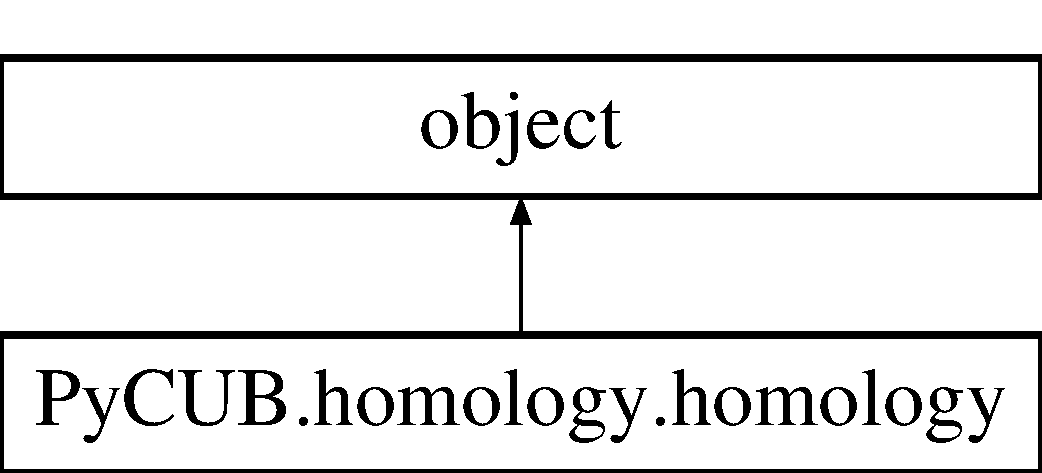
\includegraphics[height=2.000000cm]{class_py_c_u_b_1_1homology_1_1homology}
\end{center}
\end{figure}
\subsection*{Public Member Functions}
\begin{DoxyCompactItemize}
\item 
\mbox{\Hypertarget{class_py_c_u_b_1_1homology_1_1homology_a441a70cdc5814708841f5d3c29548203}\label{class_py_c_u_b_1_1homology_1_1homology_a441a70cdc5814708841f5d3c29548203}} 
def {\bfseries \+\_\+\+\_\+init\+\_\+\+\_\+} (self, kwargs)
\item 
\mbox{\Hypertarget{class_py_c_u_b_1_1homology_1_1homology_af27d98c4ced0023053744c7ba038b33a}\label{class_py_c_u_b_1_1homology_1_1homology_af27d98c4ced0023053744c7ba038b33a}} 
def {\bfseries \+\_\+\+\_\+str\+\_\+\+\_\+} (self)
\item 
def \mbox{\hyperlink{class_py_c_u_b_1_1homology_1_1homology_a32017c483bad9a5c4498640279a79634}{remove}} (self, species)
\begin{DoxyCompactList}\small\item\em removes the list of species from this homology if it exists there \end{DoxyCompactList}\item 
def \mbox{\hyperlink{class_py_c_u_b_1_1homology_1_1homology_ad430899a462da76cdd6e1fc6ee73e0ec}{nb\+\_\+unique\+\_\+species}} (self)
\begin{DoxyCompactList}\small\item\em compute the number of unique species in this homologies \end{DoxyCompactList}\item 
def \mbox{\hyperlink{class_py_c_u_b_1_1homology_1_1homology_a513d82c775ba47678304c97572eaf932}{order}} (self, withtaxons=False)
\begin{DoxyCompactList}\small\item\em order the names by numerical increasing order \end{DoxyCompactList}\item 
def \mbox{\hyperlink{class_py_c_u_b_1_1homology_1_1homology_aaeb164cd217a4746ff0082da1a92fc5e}{compute\+\_\+averages}} (self)
\begin{DoxyCompactList}\small\item\em Computes the mean, var and mean of the homology. \end{DoxyCompactList}\item 
def \mbox{\hyperlink{class_py_c_u_b_1_1homology_1_1homology_a3db21ba20b7720362cc19cc5b204eeab}{reduce\+\_\+dim}} (self, alg=\textquotesingle{}tsne\textquotesingle{}, n=2, perplexity=40)
\begin{DoxyCompactList}\small\item\em reduce the dimensionality of your gene dataset to a defined dimension using the t-\/\+S\+NE algorithm \end{DoxyCompactList}\item 
def \mbox{\hyperlink{class_py_c_u_b_1_1homology_1_1homology_a1a3802095c2ea6f426e803b055a2aea9}{plot}} (self, reducer=\char`\"{}tsne\char`\"{}, per=40, interactive=True, D=2, size=20)
\begin{DoxyCompactList}\small\item\em plot the dimensionality reduced datapoint of the homology matrix \end{DoxyCompactList}\item 
def \mbox{\hyperlink{class_py_c_u_b_1_1homology_1_1homology_a7e7748ba85bf571bb04df7a26e2c682c}{clusterize\+\_\+}} (self, clustering=\textquotesingle{}gaussian\textquotesingle{}, eps=0.\+8, homogroupnb=None, assess=True, verbose=True)
\begin{DoxyCompactList}\small\item\em will clusterize the homology using gaussian mixture clustering or D\+B\+S\+C\+AN \end{DoxyCompactList}\end{DoxyCompactItemize}
\subsection*{Public Attributes}
\begin{DoxyCompactItemize}
\item 
\mbox{\Hypertarget{class_py_c_u_b_1_1homology_1_1homology_ad0fa49f698ad9e7ae29f624d45462c4d}\label{class_py_c_u_b_1_1homology_1_1homology_ad0fa49f698ad9e7ae29f624d45462c4d}} 
{\bfseries metrics}
\item 
\mbox{\Hypertarget{class_py_c_u_b_1_1homology_1_1homology_a1eb731bc0f1f864f9bdc1b00e2038dc6}\label{class_py_c_u_b_1_1homology_1_1homology_a1eb731bc0f1f864f9bdc1b00e2038dc6}} 
{\bfseries homocode}
\item 
\mbox{\Hypertarget{class_py_c_u_b_1_1homology_1_1homology_a74a80cf95e01b8ac1f8547507481ab46}\label{class_py_c_u_b_1_1homology_1_1homology_a74a80cf95e01b8ac1f8547507481ab46}} 
{\bfseries proteinids}
\item 
\mbox{\Hypertarget{class_py_c_u_b_1_1homology_1_1homology_a0438db8bca39f5964292ea3e5f3ae519}\label{class_py_c_u_b_1_1homology_1_1homology_a0438db8bca39f5964292ea3e5f3ae519}} 
{\bfseries protein\+\_\+abundance}
\item 
\mbox{\Hypertarget{class_py_c_u_b_1_1homology_1_1homology_ae230e5a5e755ffeb7166ceef23cfaa90}\label{class_py_c_u_b_1_1homology_1_1homology_ae230e5a5e755ffeb7166ceef23cfaa90}} 
{\bfseries weight}
\item 
\mbox{\Hypertarget{class_py_c_u_b_1_1homology_1_1homology_a0290845a014043ef7cef5994da0ea14f}\label{class_py_c_u_b_1_1homology_1_1homology_a0290845a014043ef7cef5994da0ea14f}} 
{\bfseries m\+R\+N\+A\+\_\+abundance}
\item 
\mbox{\Hypertarget{class_py_c_u_b_1_1homology_1_1homology_a41ea8ca7536b4e7db86d9481f14c4c89}\label{class_py_c_u_b_1_1homology_1_1homology_a41ea8ca7536b4e7db86d9481f14c4c89}} 
{\bfseries cys\+\_\+elements}
\item 
\mbox{\Hypertarget{class_py_c_u_b_1_1homology_1_1homology_a6318ac761caa41be6b784340bc3e9d7c}\label{class_py_c_u_b_1_1homology_1_1homology_a6318ac761caa41be6b784340bc3e9d7c}} 
{\bfseries is\+\_\+secreted}
\item 
\mbox{\Hypertarget{class_py_c_u_b_1_1homology_1_1homology_a6bfbe5b4868039efca584fb13e3e17b4}\label{class_py_c_u_b_1_1homology_1_1homology_a6bfbe5b4868039efca584fb13e3e17b4}} 
{\bfseries decay\+\_\+rate}
\item 
\mbox{\Hypertarget{class_py_c_u_b_1_1homology_1_1homology_ab5b1b81d50e5bca0eac0f6bee539c4d7}\label{class_py_c_u_b_1_1homology_1_1homology_ab5b1b81d50e5bca0eac0f6bee539c4d7}} 
{\bfseries cluster}
\end{DoxyCompactItemize}
\subsection*{Static Public Attributes}
\begin{DoxyCompactItemize}
\item 
\mbox{\Hypertarget{class_py_c_u_b_1_1homology_1_1homology_a5220c03b38deb65d0e682bd1ad85802b}\label{class_py_c_u_b_1_1homology_1_1homology_a5220c03b38deb65d0e682bd1ad85802b}} 
{\bfseries full} = None
\item 
\mbox{\Hypertarget{class_py_c_u_b_1_1homology_1_1homology_af6fbc0a12aaec1fd2c4e2231d8de5520}\label{class_py_c_u_b_1_1homology_1_1homology_af6fbc0a12aaec1fd2c4e2231d8de5520}} 
{\bfseries var} = None
\item 
\mbox{\Hypertarget{class_py_c_u_b_1_1homology_1_1homology_aabb8f64472865c658c9089b6d5ff51fd}\label{class_py_c_u_b_1_1homology_1_1homology_aabb8f64472865c658c9089b6d5ff51fd}} 
{\bfseries mean} = None
\item 
\mbox{\Hypertarget{class_py_c_u_b_1_1homology_1_1homology_acf7c487a7f77ef947afc193d36becd61}\label{class_py_c_u_b_1_1homology_1_1homology_acf7c487a7f77ef947afc193d36becd61}} 
{\bfseries clusters} = None
\item 
\mbox{\Hypertarget{class_py_c_u_b_1_1homology_1_1homology_a7553f27ba7af2b61b973688bf1c72a7b}\label{class_py_c_u_b_1_1homology_1_1homology_a7553f27ba7af2b61b973688bf1c72a7b}} 
{\bfseries centroids} = None
\item 
\mbox{\Hypertarget{class_py_c_u_b_1_1homology_1_1homology_aae3f58df1a8aa3032b3bb648b5f9788a}\label{class_py_c_u_b_1_1homology_1_1homology_aae3f58df1a8aa3032b3bb648b5f9788a}} 
dictionary {\bfseries metrics} = \{\}
\item 
\mbox{\Hypertarget{class_py_c_u_b_1_1homology_1_1homology_af59d023da4ec847ead6845216b1c02f0}\label{class_py_c_u_b_1_1homology_1_1homology_af59d023da4ec847ead6845216b1c02f0}} 
string {\bfseries homocode} = \textquotesingle{}None\textquotesingle{}
\item 
\mbox{\Hypertarget{class_py_c_u_b_1_1homology_1_1homology_acbb6a5d373b79e9a783eb9efaaaecb97}\label{class_py_c_u_b_1_1homology_1_1homology_acbb6a5d373b79e9a783eb9efaaaecb97}} 
{\bfseries nans} = None
\item 
\mbox{\Hypertarget{class_py_c_u_b_1_1homology_1_1homology_a56a1f0e4e56e373d69c3d39712937278}\label{class_py_c_u_b_1_1homology_1_1homology_a56a1f0e4e56e373d69c3d39712937278}} 
{\bfseries lenmat} = None
\item 
\mbox{\Hypertarget{class_py_c_u_b_1_1homology_1_1homology_ae8979e24b36f8ca79963aa1f03db1718}\label{class_py_c_u_b_1_1homology_1_1homology_ae8979e24b36f8ca79963aa1f03db1718}} 
{\bfseries names} = None
\item 
\mbox{\Hypertarget{class_py_c_u_b_1_1homology_1_1homology_adb1c7c9de932faa407921b746fea951d}\label{class_py_c_u_b_1_1homology_1_1homology_adb1c7c9de932faa407921b746fea951d}} 
{\bfseries doub} = None
\item 
\mbox{\Hypertarget{class_py_c_u_b_1_1homology_1_1homology_a862b28ceb170090b9c9959d0ec234ecf}\label{class_py_c_u_b_1_1homology_1_1homology_a862b28ceb170090b9c9959d0ec234ecf}} 
{\bfseries G\+Ccount} = None
\item 
\mbox{\Hypertarget{class_py_c_u_b_1_1homology_1_1homology_af5cc9c64f61bf6154788e601e68ac56f}\label{class_py_c_u_b_1_1homology_1_1homology_af5cc9c64f61bf6154788e601e68ac56f}} 
{\bfseries reduced} = None
\item 
\mbox{\Hypertarget{class_py_c_u_b_1_1homology_1_1homology_a1332a6816c31c207bcf9b950b9befdd2}\label{class_py_c_u_b_1_1homology_1_1homology_a1332a6816c31c207bcf9b950b9befdd2}} 
{\bfseries reduced\+\_\+algo} = None
\item 
\mbox{\Hypertarget{class_py_c_u_b_1_1homology_1_1homology_a3d898f87bb402fff974e77a3813c91b9}\label{class_py_c_u_b_1_1homology_1_1homology_a3d898f87bb402fff974e77a3813c91b9}} 
{\bfseries Ka\+Ks\+\_\+\+Scores} = None
\item 
\mbox{\Hypertarget{class_py_c_u_b_1_1homology_1_1homology_a456033ba31e423f2844163b02441f253}\label{class_py_c_u_b_1_1homology_1_1homology_a456033ba31e423f2844163b02441f253}} 
{\bfseries similarity\+\_\+scores} = None
\item 
\mbox{\Hypertarget{class_py_c_u_b_1_1homology_1_1homology_a8d77dcd1deecff3b3114e89d50bd08d7}\label{class_py_c_u_b_1_1homology_1_1homology_a8d77dcd1deecff3b3114e89d50bd08d7}} 
list {\bfseries proteinids} = \mbox{[}$\,$\mbox{]}
\item 
\mbox{\Hypertarget{class_py_c_u_b_1_1homology_1_1homology_a25b698233f4fb598400fb725c00e2c99}\label{class_py_c_u_b_1_1homology_1_1homology_a25b698233f4fb598400fb725c00e2c99}} 
{\bfseries isrecent} = None
\item 
\mbox{\Hypertarget{class_py_c_u_b_1_1homology_1_1homology_af0f123770c60d2444ffb139acaaf5442}\label{class_py_c_u_b_1_1homology_1_1homology_af0f123770c60d2444ffb139acaaf5442}} 
{\bfseries ishighpreserved} = None
\item 
\mbox{\Hypertarget{class_py_c_u_b_1_1homology_1_1homology_add9343a07f66053ea6ee9dd5ebc275dc}\label{class_py_c_u_b_1_1homology_1_1homology_add9343a07f66053ea6ee9dd5ebc275dc}} 
{\bfseries geneids} = None
\item 
\mbox{\Hypertarget{class_py_c_u_b_1_1homology_1_1homology_aa710cdd07ec15477bb995f17f14f0ac5}\label{class_py_c_u_b_1_1homology_1_1homology_aa710cdd07ec15477bb995f17f14f0ac5}} 
{\bfseries ref} = None
\item 
\mbox{\Hypertarget{class_py_c_u_b_1_1homology_1_1homology_a3aeac1174f5e74f3291d35bfbeb0ae56}\label{class_py_c_u_b_1_1homology_1_1homology_a3aeac1174f5e74f3291d35bfbeb0ae56}} 
{\bfseries refprot} = None
\item 
\mbox{\Hypertarget{class_py_c_u_b_1_1homology_1_1homology_a549fd390f70453a9676ee4d26c84fe04}\label{class_py_c_u_b_1_1homology_1_1homology_a549fd390f70453a9676ee4d26c84fe04}} 
{\bfseries refgene} = None
\item 
\mbox{\Hypertarget{class_py_c_u_b_1_1homology_1_1homology_a7f37b98057afffafaeae13285490b229}\label{class_py_c_u_b_1_1homology_1_1homology_a7f37b98057afffafaeae13285490b229}} 
{\bfseries ecai} = None
\item 
\mbox{\Hypertarget{class_py_c_u_b_1_1homology_1_1homology_a42eb34bc6c1e774b237e479f83cd6bf7}\label{class_py_c_u_b_1_1homology_1_1homology_a42eb34bc6c1e774b237e479f83cd6bf7}} 
{\bfseries meanecai} = None
\item 
\mbox{\Hypertarget{class_py_c_u_b_1_1homology_1_1homology_a9dea84f934449466e561988ea1d2031d}\label{class_py_c_u_b_1_1homology_1_1homology_a9dea84f934449466e561988ea1d2031d}} 
{\bfseries cai} = None
\item 
\mbox{\Hypertarget{class_py_c_u_b_1_1homology_1_1homology_a97977b754401226826b71af612e6d33e}\label{class_py_c_u_b_1_1homology_1_1homology_a97977b754401226826b71af612e6d33e}} 
{\bfseries meancai} = None
\item 
\mbox{\Hypertarget{class_py_c_u_b_1_1homology_1_1homology_a5a3df5b52429c04c5bed49bd5e4a3b20}\label{class_py_c_u_b_1_1homology_1_1homology_a5a3df5b52429c04c5bed49bd5e4a3b20}} 
int {\bfseries protein\+\_\+abundance} = 0.
\item 
\mbox{\Hypertarget{class_py_c_u_b_1_1homology_1_1homology_aeb597a006a4b74e0c4332079191fddc9}\label{class_py_c_u_b_1_1homology_1_1homology_aeb597a006a4b74e0c4332079191fddc9}} 
int {\bfseries weight} = 0
\item 
\mbox{\Hypertarget{class_py_c_u_b_1_1homology_1_1homology_aa51ccde91bb3ca90cb11ae263627665a}\label{class_py_c_u_b_1_1homology_1_1homology_aa51ccde91bb3ca90cb11ae263627665a}} 
{\bfseries conservation} = None
\item 
\mbox{\Hypertarget{class_py_c_u_b_1_1homology_1_1homology_a62e7776334a677b8634faede236529de}\label{class_py_c_u_b_1_1homology_1_1homology_a62e7776334a677b8634faede236529de}} 
int {\bfseries m\+R\+N\+A\+\_\+abundance} = 0.
\item 
\mbox{\Hypertarget{class_py_c_u_b_1_1homology_1_1homology_a5492c796d1e811df903eb6ac5e6c5873}\label{class_py_c_u_b_1_1homology_1_1homology_a5492c796d1e811df903eb6ac5e6c5873}} 
int {\bfseries cys\+\_\+elements} = 0
\item 
\mbox{\Hypertarget{class_py_c_u_b_1_1homology_1_1homology_a0db815d3136df0d8057d6aa207e3a9d7}\label{class_py_c_u_b_1_1homology_1_1homology_a0db815d3136df0d8057d6aa207e3a9d7}} 
bool {\bfseries is\+\_\+secreted} = False
\item 
\mbox{\Hypertarget{class_py_c_u_b_1_1homology_1_1homology_a86cb7804faa6ffae20b7155897d88971}\label{class_py_c_u_b_1_1homology_1_1homology_a86cb7804faa6ffae20b7155897d88971}} 
int {\bfseries decay\+\_\+rate} = 0.
\item 
\mbox{\Hypertarget{class_py_c_u_b_1_1homology_1_1homology_a7b73b4cd404f7432302ce682970c04c1}\label{class_py_c_u_b_1_1homology_1_1homology_a7b73b4cd404f7432302ce682970c04c1}} 
{\bfseries tot\+\_\+volume} = None
\item 
\mbox{\Hypertarget{class_py_c_u_b_1_1homology_1_1homology_a2fcdeaac4c8dcda15c2faaa26d565c2b}\label{class_py_c_u_b_1_1homology_1_1homology_a2fcdeaac4c8dcda15c2faaa26d565c2b}} 
{\bfseries mean\+\_\+hydrophobicity} = None
\item 
\mbox{\Hypertarget{class_py_c_u_b_1_1homology_1_1homology_a3935ee71c6588e71ed71ca843dabb275}\label{class_py_c_u_b_1_1homology_1_1homology_a3935ee71c6588e71ed71ca843dabb275}} 
{\bfseries glucose\+\_\+cost} = None
\item 
\mbox{\Hypertarget{class_py_c_u_b_1_1homology_1_1homology_af6987d4b9223fb55cfe60e0456478b71}\label{class_py_c_u_b_1_1homology_1_1homology_af6987d4b9223fb55cfe60e0456478b71}} 
{\bfseries synthesis\+\_\+steps} = None
\item 
\mbox{\Hypertarget{class_py_c_u_b_1_1homology_1_1homology_ab3cc7d820ffac1600aea6dbc58995364}\label{class_py_c_u_b_1_1homology_1_1homology_ab3cc7d820ffac1600aea6dbc58995364}} 
{\bfseries isoelectricpoint} = None
\item 
\mbox{\Hypertarget{class_py_c_u_b_1_1homology_1_1homology_a0fee75b305ed6adb93ed111cce23218a}\label{class_py_c_u_b_1_1homology_1_1homology_a0fee75b305ed6adb93ed111cce23218a}} 
{\bfseries othercods} = None
\end{DoxyCompactItemize}
\subsection*{Private Member Functions}
\begin{DoxyCompactItemize}
\item 
def \mbox{\hyperlink{class_py_c_u_b_1_1homology_1_1homology_af7f186d30cb3469d73782da85f9d06bc}{\+\_\+dictify}} (self)
\begin{DoxyCompactList}\small\item\em Used by the saving function. \end{DoxyCompactList}\end{DoxyCompactItemize}


\subsection{Detailed Description}
in homology we store an homology with all its related data, 

it reduced matrix with dim reduction and its clusters for example it is supposed to be store in a dictionary of homologies an homology is a set of genes from different species related by a common ancester gene and generally a common function. the unique metadatas are generally from the reference species/genome


\begin{DoxyParams}{Parameters}
{\em names} & list of int corresponding to names in utils.\+speciestable \\
\hline
{\em full} & np.\+array\mbox{[}float\mbox{]} (species, amino) of one homology with entropy value vector per species \\
\hline
{\em reduced} & np.\+array\mbox{[}float\mbox{]} (species, x$\ast$y) of one homology dimensionality reduced \\
\hline
{\em clusters} & list\mbox{[}int\mbox{]} of cluster val for each species \\
\hline
{\em centroids} & np.\+array\mbox{[}float\mbox{]} the position in aminoacid\# Dimension of each centroids (number of centroid == number of cluster), dimension is reduced when plotted \\
\hline
{\em metrics} & a dict of metrics names and values for the cluster of this homology \\
\hline
{\em nans} & np.\+array\mbox{[}bool\mbox{]} wether or not this position is a nan \\
\hline
{\em lenmat} & a np.\+array\mbox{[}int\mbox{]} species amino of int of length of each amino acids (number) \\
\hline
{\em doub} & np.\+array\mbox{[}bool\mbox{]} of wether or not this position is a doublon ( a copy number of the gene for the species) \\
\hline
{\em reduced\+\_\+algo} & str dimensionality reduction algorithm used on this homology \\
\hline
{\em var} & np.\+array of the variance in the C\+UB value for each datapoint \\
\hline
{\em mean} & np.\+array\mbox{[}float\mbox{]} of the mean C\+UB for each datapoint \\
\hline
{\em homocode} & str the code of the homology \\
\hline
{\em G\+Ccount} & np.\+array\mbox{[}float\mbox{]} GC bias for each datapoint \\
\hline
{\em Ka\+Ks\+\_\+\+Scores} & np.\+array\mbox{[}float\mbox{]} a form of similarity score between genes/datapoints \\
\hline
{\em similarity\+\_\+scores} & np.\+array\mbox{[}float\mbox{]} similarity score between genes/datapoints \\
\hline
{\em proteinids} & list\mbox{[}str\mbox{]} the protein names for each datapoints \\
\hline
{\em isrecent} & float a proxy for wether or not this homology has appeated recently \\
\hline
{\em ishighpreserved} & bool a proxy for wether or not this homology is conserved throughout evolution \\
\hline
{\em geneids} & list\mbox{[}str\mbox{]} the name of the genes \\
\hline
{\em ref} & np.\+array\mbox{[}float\mbox{]} the reference C\+UB value of cerevisiae gene \\
\hline
{\em refprot} & str the reference protein name of cerevisiae gene \\
\hline
{\em refgene} & str the reference gene name of cerevisiae gene \\
\hline
{\em ecai} & np.\+array\mbox{[}float\mbox{]} the codon adaptation index of each gene \\
\hline
{\em meanecai} & float the mean ecai of the ecai \\
\hline
{\em protein\+\_\+abundance} & float the average abundance of the protein enoded by this gene in cerevisiae cells \\
\hline
{\em weight} & int the molecular weight of this protein \\
\hline
{\em m\+R\+N\+A\+\_\+abundance} & float the average abundance of the messenger R\+NA of this coding gene in cerevisiae cells \\
\hline
{\em cys\+\_\+elements} & int the number of cys regulatory elements known for cerevisiae on this gene (the value is only referenced for secreted genes) \\
\hline
{\em is\+\_\+secreted} & bool wether or not this protein is secreted out of the cell \\
\hline
{\em decay\+\_\+rate} & float the half life in minute of this protein \\
\hline
{\em tot\+\_\+volume} & int a proxy of the molecular volume of this protein \\
\hline
{\em mean\+\_\+hydrophobicity} & a very distant proxy of the hydrophobicity of this protein \\
\hline
{\em glucose\+\_\+cost} & the glucose cost of creating the amino acids required to build up this protein \\
\hline
{\em synthesis\+\_\+steps} & the number of steps required by the cell to build up the amino acids of this protein \\
\hline
{\em isoelectricpoint} & float, a proxy of the Pi of this protein. \\
\hline
{\em conservation} & float, the total conservation of each amino of the corresponding protein \\
\hline
{\em othercods} & float, the average number of codons other than the ones of the 18 amino acids we are looking at per species on the homology \\
\hline
\end{DoxyParams}


\subsection{Member Function Documentation}
\mbox{\Hypertarget{class_py_c_u_b_1_1homology_1_1homology_af7f186d30cb3469d73782da85f9d06bc}\label{class_py_c_u_b_1_1homology_1_1homology_af7f186d30cb3469d73782da85f9d06bc}} 
\index{Py\+C\+U\+B\+::homology\+::homology@{Py\+C\+U\+B\+::homology\+::homology}!\+\_\+dictify@{\+\_\+dictify}}
\index{\+\_\+dictify@{\+\_\+dictify}!Py\+C\+U\+B\+::homology\+::homology@{Py\+C\+U\+B\+::homology\+::homology}}
\subsubsection{\texorpdfstring{\+\_\+dictify()}{\_dictify()}}
{\footnotesize\ttfamily def Py\+C\+U\+B.\+homology.\+homology.\+\_\+dictify (\begin{DoxyParamCaption}\item[{}]{self }\end{DoxyParamCaption})\hspace{0.3cm}{\ttfamily [private]}}



Used by the saving function. 

transform the object into a dictionary that can be json serializable


\begin{DoxyParams}{Parameters}
{\em None} & \\
\hline
\end{DoxyParams}
\begin{DoxyReturn}{Returns}
A dict holding every element to be jsonized 
\end{DoxyReturn}


Referenced by Py\+C\+U\+B.\+homology.\+homology.\+clusterize\+\_\+(), and Py\+C\+U\+B.\+py\+C\+U\+B.\+Py\+C\+U\+B.\+save().

\mbox{\Hypertarget{class_py_c_u_b_1_1homology_1_1homology_a7e7748ba85bf571bb04df7a26e2c682c}\label{class_py_c_u_b_1_1homology_1_1homology_a7e7748ba85bf571bb04df7a26e2c682c}} 
\index{Py\+C\+U\+B\+::homology\+::homology@{Py\+C\+U\+B\+::homology\+::homology}!clusterize\+\_\+@{clusterize\+\_\+}}
\index{clusterize\+\_\+@{clusterize\+\_\+}!Py\+C\+U\+B\+::homology\+::homology@{Py\+C\+U\+B\+::homology\+::homology}}
\subsubsection{\texorpdfstring{clusterize\+\_\+()}{clusterize\_()}}
{\footnotesize\ttfamily def Py\+C\+U\+B.\+homology.\+homology.\+clusterize\+\_\+ (\begin{DoxyParamCaption}\item[{}]{self,  }\item[{}]{clustering = {\ttfamily \textquotesingle{}gaussian\textquotesingle{}},  }\item[{}]{eps = {\ttfamily 0.8},  }\item[{}]{homogroupnb = {\ttfamily None},  }\item[{}]{assess = {\ttfamily True},  }\item[{}]{verbose = {\ttfamily True} }\end{DoxyParamCaption})}



will clusterize the homology using gaussian mixture clustering or D\+B\+S\+C\+AN 

and order them according to the density of each cluster (we are interested in the dense ones) and assess the quality using 3 criterion\+: B\+IC, A\+IC ,silhouette, cal\+\_\+hara, phylodistance.


\begin{DoxyParams}{Parameters}
{\em clustering} & str flag the clustering algorithm \mbox{[}gaussian, dbscan\mbox{]} \\
\hline
{\em eps} & float, hyperparam of the max size of the nsphere of each cluster \\
\hline
{\em homogroupnb} & int hyperparam of gaussian for the number of clusters \\
\hline
{\em assess} & wether or not to assess the quality of the clustering \\
\hline
{\em verbose} & wether or not to show clustering quality information\\
\hline
\end{DoxyParams}
\begin{DoxyReturn}{Returns}
The clusters for each datapoint of the homology as a list\mbox{[}int\mbox{]}
\end{DoxyReturn}

\begin{DoxyExceptions}{Exceptions}
{\em Attribute\+Error} & \char`\"{}\+Hey, please use gaussian or dbscan\char`\"{} \\
\hline
\end{DoxyExceptions}


Referenced by Py\+C\+U\+B.\+homology.\+homology.\+plot().

\mbox{\Hypertarget{class_py_c_u_b_1_1homology_1_1homology_aaeb164cd217a4746ff0082da1a92fc5e}\label{class_py_c_u_b_1_1homology_1_1homology_aaeb164cd217a4746ff0082da1a92fc5e}} 
\index{Py\+C\+U\+B\+::homology\+::homology@{Py\+C\+U\+B\+::homology\+::homology}!compute\+\_\+averages@{compute\+\_\+averages}}
\index{compute\+\_\+averages@{compute\+\_\+averages}!Py\+C\+U\+B\+::homology\+::homology@{Py\+C\+U\+B\+::homology\+::homology}}
\subsubsection{\texorpdfstring{compute\+\_\+averages()}{compute\_averages()}}
{\footnotesize\ttfamily def Py\+C\+U\+B.\+homology.\+homology.\+compute\+\_\+averages (\begin{DoxyParamCaption}\item[{}]{self }\end{DoxyParamCaption})}



Computes the mean, var and mean of the homology. 


\begin{DoxyParams}{Parameters}
{\em None} & \\
\hline
\end{DoxyParams}


Referenced by Py\+C\+U\+B.\+homology.\+homology.\+order().

\mbox{\Hypertarget{class_py_c_u_b_1_1homology_1_1homology_ad430899a462da76cdd6e1fc6ee73e0ec}\label{class_py_c_u_b_1_1homology_1_1homology_ad430899a462da76cdd6e1fc6ee73e0ec}} 
\index{Py\+C\+U\+B\+::homology\+::homology@{Py\+C\+U\+B\+::homology\+::homology}!nb\+\_\+unique\+\_\+species@{nb\+\_\+unique\+\_\+species}}
\index{nb\+\_\+unique\+\_\+species@{nb\+\_\+unique\+\_\+species}!Py\+C\+U\+B\+::homology\+::homology@{Py\+C\+U\+B\+::homology\+::homology}}
\subsubsection{\texorpdfstring{nb\+\_\+unique\+\_\+species()}{nb\_unique\_species()}}
{\footnotesize\ttfamily def Py\+C\+U\+B.\+homology.\+homology.\+nb\+\_\+unique\+\_\+species (\begin{DoxyParamCaption}\item[{}]{self }\end{DoxyParamCaption})}



compute the number of unique species in this homologies 

(basically count the number of doub)


\begin{DoxyParams}{Parameters}
{\em None} & \\
\hline
\end{DoxyParams}
\begin{DoxyReturn}{Returns}
The number of unique species in this homology 
\end{DoxyReturn}


Referenced by Py\+C\+U\+B.\+homology.\+homology.\+remove().

\mbox{\Hypertarget{class_py_c_u_b_1_1homology_1_1homology_a513d82c775ba47678304c97572eaf932}\label{class_py_c_u_b_1_1homology_1_1homology_a513d82c775ba47678304c97572eaf932}} 
\index{Py\+C\+U\+B\+::homology\+::homology@{Py\+C\+U\+B\+::homology\+::homology}!order@{order}}
\index{order@{order}!Py\+C\+U\+B\+::homology\+::homology@{Py\+C\+U\+B\+::homology\+::homology}}
\subsubsection{\texorpdfstring{order()}{order()}}
{\footnotesize\ttfamily def Py\+C\+U\+B.\+homology.\+homology.\+order (\begin{DoxyParamCaption}\item[{}]{self,  }\item[{}]{withtaxons = {\ttfamily False} }\end{DoxyParamCaption})}



order the names by numerical increasing order 

and sorts every representations as well according to this ordering


\begin{DoxyParams}{Parameters}
{\em withtaxons} & bool to true if there is taxonomic data (present before preprocessing) \\
\hline
\end{DoxyParams}


Referenced by Py\+C\+U\+B.\+homology.\+homology.\+nb\+\_\+unique\+\_\+species().

\mbox{\Hypertarget{class_py_c_u_b_1_1homology_1_1homology_a1a3802095c2ea6f426e803b055a2aea9}\label{class_py_c_u_b_1_1homology_1_1homology_a1a3802095c2ea6f426e803b055a2aea9}} 
\index{Py\+C\+U\+B\+::homology\+::homology@{Py\+C\+U\+B\+::homology\+::homology}!plot@{plot}}
\index{plot@{plot}!Py\+C\+U\+B\+::homology\+::homology@{Py\+C\+U\+B\+::homology\+::homology}}
\subsubsection{\texorpdfstring{plot()}{plot()}}
{\footnotesize\ttfamily def Py\+C\+U\+B.\+homology.\+homology.\+plot (\begin{DoxyParamCaption}\item[{}]{self,  }\item[{}]{reducer = {\ttfamily \char`\"{}tsne\char`\"{}},  }\item[{}]{per = {\ttfamily 40},  }\item[{}]{interactive = {\ttfamily True},  }\item[{}]{D = {\ttfamily 2},  }\item[{}]{size = {\ttfamily 20} }\end{DoxyParamCaption})}



plot the dimensionality reduced datapoint of the homology matrix 

colors represents the different clusters you can set the interactivity to gain deeper knowledge of the dataset. It can dim reduce the data and will also save the figure in utils/save. Moreover, it will print some interesting data about the homology


\begin{DoxyParams}{Parameters}
{\em reducer} & str flag the algorithm to reduce the matrix of utils.\+cubD to D D \\
\hline
{\em per} & int he perplexity when using tsne algorithm \\
\hline
{\em size} & int the size of the plot \\
\hline
{\em interactive} & (recommended) wether to use bokeh or not to represend the data will show name of the species when hovering over datapoint will show a gradient of evolutionary distance of the species of the datapoint currently hovered to each other species \\
\hline
{\em D} & int the goal dimension (2-\/3-\/4) when using matplotlib\\
\hline
\end{DoxyParams}
\begin{DoxyReturn}{Returns}
The plot interactive or not and some informations (as prints)
\end{DoxyReturn}

\begin{DoxyExceptions}{Exceptions}
{\em Unbound\+Local\+Error} & \char`\"{}you need to have dimensionality reduced to 2\+D to have a right plotting of the centroids\char`\"{} \\
\hline
\end{DoxyExceptions}


Referenced by Py\+C\+U\+B.\+homology.\+homology.\+reduce\+\_\+dim().

\mbox{\Hypertarget{class_py_c_u_b_1_1homology_1_1homology_a3db21ba20b7720362cc19cc5b204eeab}\label{class_py_c_u_b_1_1homology_1_1homology_a3db21ba20b7720362cc19cc5b204eeab}} 
\index{Py\+C\+U\+B\+::homology\+::homology@{Py\+C\+U\+B\+::homology\+::homology}!reduce\+\_\+dim@{reduce\+\_\+dim}}
\index{reduce\+\_\+dim@{reduce\+\_\+dim}!Py\+C\+U\+B\+::homology\+::homology@{Py\+C\+U\+B\+::homology\+::homology}}
\subsubsection{\texorpdfstring{reduce\+\_\+dim()}{reduce\_dim()}}
{\footnotesize\ttfamily def Py\+C\+U\+B.\+homology.\+homology.\+reduce\+\_\+dim (\begin{DoxyParamCaption}\item[{}]{self,  }\item[{}]{alg = {\ttfamily \textquotesingle{}tsne\textquotesingle{}},  }\item[{}]{n = {\ttfamily 2},  }\item[{}]{perplexity = {\ttfamily 40} }\end{DoxyParamCaption})}



reduce the dimensionality of your gene dataset to a defined dimension using the t-\/\+S\+NE algorithm 


\begin{DoxyParams}{Parameters}
{\em alg} & a matrix of gene codon usage per species \\
\hline
{\em n} & the desired dimension \\
\hline
{\em perplexity} & an optional value when you know about tsne\\
\hline
\end{DoxyParams}
\begin{DoxyReturn}{Returns}
The reduced dataset 
\end{DoxyReturn}


Referenced by Py\+C\+U\+B.\+homology.\+homology.\+compute\+\_\+averages(), and Py\+C\+U\+B.\+homology.\+homology.\+plot().

\mbox{\Hypertarget{class_py_c_u_b_1_1homology_1_1homology_a32017c483bad9a5c4498640279a79634}\label{class_py_c_u_b_1_1homology_1_1homology_a32017c483bad9a5c4498640279a79634}} 
\index{Py\+C\+U\+B\+::homology\+::homology@{Py\+C\+U\+B\+::homology\+::homology}!remove@{remove}}
\index{remove@{remove}!Py\+C\+U\+B\+::homology\+::homology@{Py\+C\+U\+B\+::homology\+::homology}}
\subsubsection{\texorpdfstring{remove()}{remove()}}
{\footnotesize\ttfamily def Py\+C\+U\+B.\+homology.\+homology.\+remove (\begin{DoxyParamCaption}\item[{}]{self,  }\item[{}]{species }\end{DoxyParamCaption})}



removes the list of species from this homology if it exists there 


\begin{DoxyParams}{Parameters}
{\em species} & list\mbox{[}str\mbox{]} of species to remove \\
\hline
\end{DoxyParams}


Referenced by Py\+C\+U\+B.\+homoset.\+Homo\+Set.\+clean\+\_\+species().



The documentation for this class was generated from the following file\+:\begin{DoxyCompactItemize}
\item 
Py\+C\+U\+B/homology.\+py\end{DoxyCompactItemize}

\hypertarget{class_py_c_u_b_1_1homoset_1_1_homo_set}{}\section{Py\+C\+U\+B.\+homoset.\+Homo\+Set Class Reference}
\label{class_py_c_u_b_1_1homoset_1_1_homo_set}\index{Py\+C\+U\+B.\+homoset.\+Homo\+Set@{Py\+C\+U\+B.\+homoset.\+Homo\+Set}}


\mbox{\hyperlink{class_py_c_u_b_1_1homoset_1_1_homo_set}{Homo\+Set}} is the object containing evrey homology as a dictionnary according to thie rhomology code.  


Inheritance diagram for Py\+C\+U\+B.\+homoset.\+Homo\+Set\+:\begin{figure}[H]
\begin{center}
\leavevmode
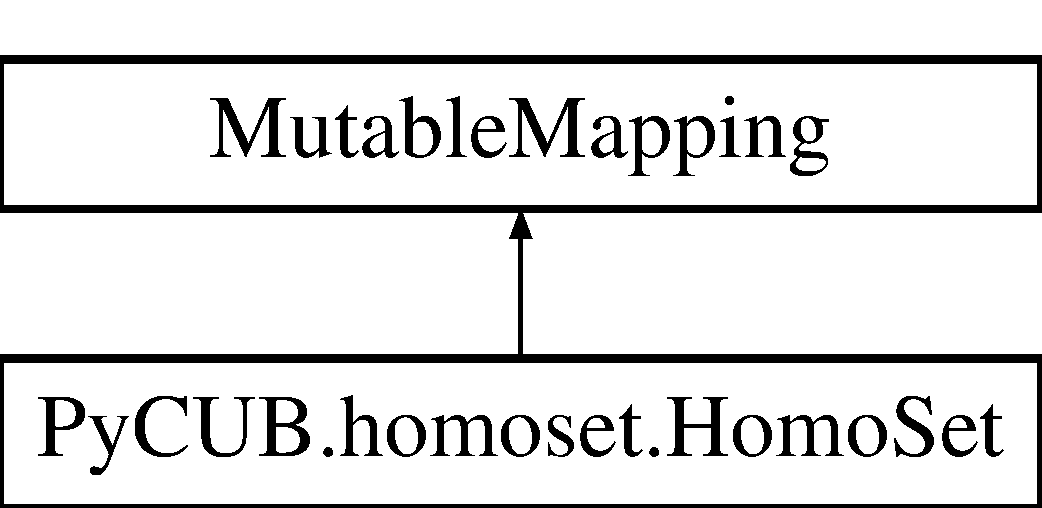
\includegraphics[height=2.000000cm]{class_py_c_u_b_1_1homoset_1_1_homo_set}
\end{center}
\end{figure}
\subsection*{Public Member Functions}
\begin{DoxyCompactItemize}
\item 
def \mbox{\hyperlink{class_py_c_u_b_1_1homoset_1_1_homo_set_adbe4d9e4087fe5b53d861476c011329d}{\+\_\+\+\_\+init\+\_\+\+\_\+}} (self, kwargs)
\begin{DoxyCompactList}\small\item\em will initialize the object with the different values you might have from another project use the data dictionnary to add any type of data \end{DoxyCompactList}\item 
def \mbox{\hyperlink{class_py_c_u_b_1_1homoset_1_1_homo_set_ab7ac33ea3033b440816e179cb4a5e3c0}{\+\_\+\+\_\+getitem\+\_\+\+\_\+}} (self, key)
\begin{DoxyCompactList}\small\item\em get the homology at the corresponding key \end{DoxyCompactList}\item 
def \mbox{\hyperlink{class_py_c_u_b_1_1homoset_1_1_homo_set_a42a7e7dc7ddb4b5717084cb093f90774}{\+\_\+\+\_\+setitem\+\_\+\+\_\+}} (self, key, value)
\begin{DoxyCompactList}\small\item\em add an item at the corresponding key \end{DoxyCompactList}\item 
\mbox{\Hypertarget{class_py_c_u_b_1_1homoset_1_1_homo_set_a5211ffec9061ca49c771d070048524a1}\label{class_py_c_u_b_1_1homoset_1_1_homo_set_a5211ffec9061ca49c771d070048524a1}} 
def {\bfseries \+\_\+\+\_\+delitem\+\_\+\+\_\+} (self, key)
\item 
\mbox{\Hypertarget{class_py_c_u_b_1_1homoset_1_1_homo_set_a2d35b1436a2bbdaea69454ffbf648bf0}\label{class_py_c_u_b_1_1homoset_1_1_homo_set_a2d35b1436a2bbdaea69454ffbf648bf0}} 
def {\bfseries \+\_\+\+\_\+iter\+\_\+\+\_\+} (self)
\item 
\mbox{\Hypertarget{class_py_c_u_b_1_1homoset_1_1_homo_set_aefca94ad0e64bcad582edcc163bc21ad}\label{class_py_c_u_b_1_1homoset_1_1_homo_set_aefca94ad0e64bcad582edcc163bc21ad}} 
def {\bfseries iteritems} (self)
\item 
\mbox{\Hypertarget{class_py_c_u_b_1_1homoset_1_1_homo_set_ada72dc2741d84a8c617dc23449154fc2}\label{class_py_c_u_b_1_1homoset_1_1_homo_set_ada72dc2741d84a8c617dc23449154fc2}} 
def {\bfseries \+\_\+\+\_\+len\+\_\+\+\_\+} (self)
\item 
def \mbox{\hyperlink{class_py_c_u_b_1_1homoset_1_1_homo_set_a8cf76800f047841bf63d507fb1b54048}{update}} (self, val)
\begin{DoxyCompactList}\small\item\em a function to update the dictionnary that homoset is \end{DoxyCompactList}\item 
def \mbox{\hyperlink{class_py_c_u_b_1_1homoset_1_1_homo_set_af57de86adab3635645d684b89636cd5c}{plot\+\_\+all}} (self, With=\textquotesingle{}tsne\textquotesingle{}, perplexity=60, interactive=False, bins=100, offset=20, iteration=400, redo=False, bypasstsne=False, dotsize=7, inpar=True)
\begin{DoxyCompactList}\small\item\em will plot all the homologies in the full\+\_\+homo\+\_\+matrix (and compute it) \end{DoxyCompactList}\item 
def \mbox{\hyperlink{class_py_c_u_b_1_1homoset_1_1_homo_set_a5029dbdf4e7f61bd38b6273f4fde9ead}{loadfullhomo}} (self)
\begin{DoxyCompactList}\small\item\em function to concatenate all the homologies in one big array(practicle for certain computations) \end{DoxyCompactList}\item 
def \mbox{\hyperlink{class_py_c_u_b_1_1homoset_1_1_homo_set_a5a56a99b5bf87afb418a1bbc5ec1c10b}{loadhashomo}} (self, withnames=False)
\begin{DoxyCompactList}\small\item\em function to compute the matrix of bool saying wether species X has a gene or more in homology Y \end{DoxyCompactList}\item 
def \mbox{\hyperlink{class_py_c_u_b_1_1homoset_1_1_homo_set_a000511647e3f85d8abadcdddaddfb04d}{size}} (self)
\begin{DoxyCompactList}\small\item\em the size of the homoset (number of genes) \end{DoxyCompactList}\item 
def \mbox{\hyperlink{class_py_c_u_b_1_1homoset_1_1_homo_set_a05935a3f03f2e2b61b2f3e7e0222e2a9}{add\+\_\+random\+\_\+homology}} (self)
\begin{DoxyCompactList}\small\item\em a function to populate a homology with random values \end{DoxyCompactList}\item 
def \mbox{\hyperlink{class_py_c_u_b_1_1homoset_1_1_homo_set_a3f689e03251e7b4fe262a86d08946998}{preprocessing}} (self, withtaxons=False, withnames=True)
\begin{DoxyCompactList}\small\item\em will compute the full list of names, \end{DoxyCompactList}\item 
\mbox{\Hypertarget{class_py_c_u_b_1_1homoset_1_1_homo_set_aa39455620288b4912e5540491913e792}\label{class_py_c_u_b_1_1homoset_1_1_homo_set_aa39455620288b4912e5540491913e792}} 
def {\bfseries preprocessing\+\_\+taxons} (self)
\item 
def \mbox{\hyperlink{class_py_c_u_b_1_1homoset_1_1_homo_set_a36cf71a7bc24b788c4d526591a8ec376}{preprocessing\+\_\+names}} (self)
\begin{DoxyCompactList}\small\item\em same as preprocessing\+\_\+taxons() but admiting there is no taxon information (Yun\textquotesingle{}s data for example) \end{DoxyCompactList}\item 
def \mbox{\hyperlink{class_py_c_u_b_1_1homoset_1_1_homo_set_a4060c440127aa861c17b6157c81e2d27}{preprocessing\+\_\+namelist}} (self)
\begin{DoxyCompactList}\small\item\em same as \mbox{\hyperlink{class_py_c_u_b_1_1homoset_1_1_homo_set_a36cf71a7bc24b788c4d526591a8ec376}{preprocessing\+\_\+names()}} but without preprocessing the names of each homologies only updating the species\+\_\+namelist \end{DoxyCompactList}\item 
def \mbox{\hyperlink{class_py_c_u_b_1_1homoset_1_1_homo_set_a59a0c4c70f6dbd2dd156e2b2c9b00421}{compute\+\_\+ages}} (self, preserved=True, minpreserv=0.\+9, minsimi=0.\+85)
\begin{DoxyCompactList}\small\item\em will compute whether or not a coding gene is highly preserved and if not how recent it is \end{DoxyCompactList}\item 
def \mbox{\hyperlink{class_py_c_u_b_1_1homoset_1_1_homo_set_a78ab39ddfa288661f5e809ea0a455187}{compute\+\_\+entropyloc}} (self, using=\textquotesingle{}computejerem\textquotesingle{})
\begin{DoxyCompactList}\small\item\em called if need entropy location and used ensembl data. \end{DoxyCompactList}\item 
def \mbox{\hyperlink{class_py_c_u_b_1_1homoset_1_1_homo_set_af19ffd1cceb4b222e642713456b300a1}{remove}} (self, species)
\begin{DoxyCompactList}\small\item\em remove this list of species from the homologies \end{DoxyCompactList}\item 
def \mbox{\hyperlink{class_py_c_u_b_1_1homoset_1_1_homo_set_a2062c7f9c3c956d43172e1688504826a}{clean\+\_\+species}} (self, thresh=0.\+3)
\begin{DoxyCompactList}\small\item\em will remove a species from all the homologies of this homoset \end{DoxyCompactList}\item 
\mbox{\Hypertarget{class_py_c_u_b_1_1homoset_1_1_homo_set_a2b4bf6cef1b2545373be7ef11c329796}\label{class_py_c_u_b_1_1homoset_1_1_homo_set_a2b4bf6cef1b2545373be7ef11c329796}} 
def \mbox{\hyperlink{class_py_c_u_b_1_1homoset_1_1_homo_set_a2b4bf6cef1b2545373be7ef11c329796}{plot\+\_\+homoperspecies}} (self)
\begin{DoxyCompactList}\small\item\em will plot the number of homology per spcies in this homology group \end{DoxyCompactList}\item 
\mbox{\Hypertarget{class_py_c_u_b_1_1homoset_1_1_homo_set_a2cd71ff76ae8cd4ed1bdc206346942d4}\label{class_py_c_u_b_1_1homoset_1_1_homo_set_a2cd71ff76ae8cd4ed1bdc206346942d4}} 
def \mbox{\hyperlink{class_py_c_u_b_1_1homoset_1_1_homo_set_a2cd71ff76ae8cd4ed1bdc206346942d4}{plot\+\_\+speciesperhomo}} (self)
\begin{DoxyCompactList}\small\item\em will plot the number of species per homologies in this homology group \end{DoxyCompactList}\item 
def \mbox{\hyperlink{class_py_c_u_b_1_1homoset_1_1_homo_set_a2d543ce742d6a4e968e14b1471319287}{cluster\+\_\+homologies}} (self, clustering=\textquotesingle{}kmeans\textquotesingle{}, byspecie=False, order=True, plot\+\_\+ordering=True, homogroupnb=2, findnb=False)
\begin{DoxyCompactList}\small\item\em Compute an homology group \+: \end{DoxyCompactList}\item 
def \mbox{\hyperlink{class_py_c_u_b_1_1homoset_1_1_homo_set_abebd6a9804b73a10fc726974630e5d26}{orderfromclust}} (self, homogroupnb, clust, byspecie=False, plot\+\_\+ordering=True)
\begin{DoxyCompactList}\small\item\em creates an ordering of every elements \end{DoxyCompactList}\item 
def \mbox{\hyperlink{class_py_c_u_b_1_1homoset_1_1_homo_set_aa41e2430673cf29f96a522e03040ca1d}{get\+\_\+clusterstats}} (self, sort=True, interactive=True, redo=False)
\begin{DoxyCompactList}\small\item\em will find the number of cluster i per homologies and per species \end{DoxyCompactList}\item 
def \mbox{\hyperlink{class_py_c_u_b_1_1homoset_1_1_homo_set_ae429c30197127c5d6248c94dbb6dfc46}{compare\+\_\+clusters}} (self, cubdistance\+\_\+matrix=True, plot=True, interactive=True, \mbox{\hyperlink{class_py_c_u_b_1_1homoset_1_1_homo_set_a000511647e3f85d8abadcdddaddfb04d}{size}}=40)
\begin{DoxyCompactList}\small\item\em for each clusters in homologies, will compare them with a similarity matrix and a distance matrix \end{DoxyCompactList}\item 
def \mbox{\hyperlink{class_py_c_u_b_1_1homoset_1_1_homo_set_a81b40822ff0d1d3e0cfccd6c3c54cdd6}{find\+\_\+clusters}} (self, clustering=\textquotesingle{}dbscan\textquotesingle{}, homogroupnb=None, assess=True, eps=0.\+8, best\+\_\+eps=True, trainingset=30, epoch=20, ranges=\mbox{[}0.\+2, \mbox{\hyperlink{class_py_c_u_b_1_1homoset_1_1_homo_set_a000511647e3f85d8abadcdddaddfb04d}{size}}=10, redo=False)
\begin{DoxyCompactList}\small\item\em Finds, for each homologies in the working homoset, groups that are part of compact clusters. \end{DoxyCompactList}\item 
def \mbox{\hyperlink{class_py_c_u_b_1_1homoset_1_1_homo_set_a36e6e64142f4cc63425f145a1754d1d6}{findbest\+\_\+eps}} (self, trainingset=400, clustering=\char`\"{}dbscan\char`\"{}, epoch=20, ranges=\mbox{[}0.\+2, \mbox{\hyperlink{class_py_c_u_b_1_1homoset_1_1_homo_set_a000511647e3f85d8abadcdddaddfb04d}{size}}=10, redo=False)
\begin{DoxyCompactList}\small\item\em will find the best eps hyperparameter (the one that minimizes the evolutionary distance within its clusters) \end{DoxyCompactList}\item 
def \mbox{\hyperlink{class_py_c_u_b_1_1homoset_1_1_homo_set_a8ab62bae7be17abf4b13ad37d5c881eb}{plot\+\_\+hashomo}} (self, invert=False, \mbox{\hyperlink{class_py_c_u_b_1_1homoset_1_1_homo_set_a000511647e3f85d8abadcdddaddfb04d}{size}}=40, interactive=False, rangeto=None)
\begin{DoxyCompactList}\small\item\em plot the has homo matrix \end{DoxyCompactList}\item 
def \mbox{\hyperlink{class_py_c_u_b_1_1homoset_1_1_homo_set_a87fcd4602c943c98543e2bc552502663}{plot\+\_\+simiclust}} (self, interactive=True, \mbox{\hyperlink{class_py_c_u_b_1_1homoset_1_1_homo_set_a000511647e3f85d8abadcdddaddfb04d}{size}}=40)
\begin{DoxyCompactList}\small\item\em plot the similarity matrix of each homologies from its clusters \end{DoxyCompactList}\item 
def \mbox{\hyperlink{class_py_c_u_b_1_1homoset_1_1_homo_set_aa385d8acea32381efae12c219c24a331}{plot\+\_\+distcub}} (self, interactive=False, \mbox{\hyperlink{class_py_c_u_b_1_1homoset_1_1_homo_set_a000511647e3f85d8abadcdddaddfb04d}{size}}=40)
\begin{DoxyCompactList}\small\item\em plot the distance matrix of each homologies from the average of their C\+UB distances \end{DoxyCompactList}\end{DoxyCompactItemize}
\subsection*{Public Attributes}
\begin{DoxyCompactItemize}
\item 
\mbox{\Hypertarget{class_py_c_u_b_1_1homoset_1_1_homo_set_acbfe58dd06d4c6ca61a528ddfabee3d6}\label{class_py_c_u_b_1_1homoset_1_1_homo_set_acbfe58dd06d4c6ca61a528ddfabee3d6}} 
{\bfseries homo\+\_\+namelist}
\item 
\mbox{\Hypertarget{class_py_c_u_b_1_1homoset_1_1_homo_set_a141708f3582bf009ec08b111124589b1}\label{class_py_c_u_b_1_1homoset_1_1_homo_set_a141708f3582bf009ec08b111124589b1}} 
{\bfseries species\+\_\+namelist}
\item 
\mbox{\Hypertarget{class_py_c_u_b_1_1homoset_1_1_homo_set_a7e0bb4c43fb89bb5165f509048a5025b}\label{class_py_c_u_b_1_1homoset_1_1_homo_set_a7e0bb4c43fb89bb5165f509048a5025b}} 
{\bfseries homogroupnb}
\item 
\mbox{\Hypertarget{class_py_c_u_b_1_1homoset_1_1_homo_set_a1e216b6dd586b4d71d48db2bd9e82fd1}\label{class_py_c_u_b_1_1homoset_1_1_homo_set_a1e216b6dd586b4d71d48db2bd9e82fd1}} 
{\bfseries clusters}
\item 
\mbox{\Hypertarget{class_py_c_u_b_1_1homoset_1_1_homo_set_a7b5672c7d4faf1bec55d7afffc13ff2a}\label{class_py_c_u_b_1_1homoset_1_1_homo_set_a7b5672c7d4faf1bec55d7afffc13ff2a}} 
{\bfseries datatype}
\item 
\mbox{\Hypertarget{class_py_c_u_b_1_1homoset_1_1_homo_set_a28336c404d04628639692b2254c4c7f4}\label{class_py_c_u_b_1_1homoset_1_1_homo_set_a28336c404d04628639692b2254c4c7f4}} 
{\bfseries phylo\+\_\+distances}
\item 
\mbox{\Hypertarget{class_py_c_u_b_1_1homoset_1_1_homo_set_a5835f6f6921772dd599c4deee9e01b35}\label{class_py_c_u_b_1_1homoset_1_1_homo_set_a5835f6f6921772dd599c4deee9e01b35}} 
{\bfseries best\+\_\+eps}
\item 
\mbox{\Hypertarget{class_py_c_u_b_1_1homoset_1_1_homo_set_ade27fdf472815f4fb2eb1d1ef552ad42}\label{class_py_c_u_b_1_1homoset_1_1_homo_set_ade27fdf472815f4fb2eb1d1ef552ad42}} 
{\bfseries wasclusterized}
\item 
\mbox{\Hypertarget{class_py_c_u_b_1_1homoset_1_1_homo_set_a25c653d5b412d60a7c3663e327b222cf}\label{class_py_c_u_b_1_1homoset_1_1_homo_set_a25c653d5b412d60a7c3663e327b222cf}} 
{\bfseries stats}
\item 
\mbox{\Hypertarget{class_py_c_u_b_1_1homoset_1_1_homo_set_ad09211d828ad602a1e3806829eb96f04}\label{class_py_c_u_b_1_1homoset_1_1_homo_set_ad09211d828ad602a1e3806829eb96f04}} 
{\bfseries homodict}
\item 
\mbox{\Hypertarget{class_py_c_u_b_1_1homoset_1_1_homo_set_ae0885604920c67cd0bf29e93a7cf4a5a}\label{class_py_c_u_b_1_1homoset_1_1_homo_set_ae0885604920c67cd0bf29e93a7cf4a5a}} 
{\bfseries cluster\+\_\+similarity}
\item 
\mbox{\Hypertarget{class_py_c_u_b_1_1homoset_1_1_homo_set_a66fe1cab79f6c84cd93ba95a9b233f0e}\label{class_py_c_u_b_1_1homoset_1_1_homo_set_a66fe1cab79f6c84cd93ba95a9b233f0e}} 
{\bfseries cub\+\_\+similarity}
\end{DoxyCompactItemize}
\subsection*{Static Public Attributes}
\begin{DoxyCompactItemize}
\item 
\mbox{\Hypertarget{class_py_c_u_b_1_1homoset_1_1_homo_set_a7c35df6a1db3f4b64a91be2417610c9e}\label{class_py_c_u_b_1_1homoset_1_1_homo_set_a7c35df6a1db3f4b64a91be2417610c9e}} 
{\bfseries hashomo\+\_\+matrix} = None
\item 
\mbox{\Hypertarget{class_py_c_u_b_1_1homoset_1_1_homo_set_a092f90e457bce969aa9c012cd971fbb4}\label{class_py_c_u_b_1_1homoset_1_1_homo_set_a092f90e457bce969aa9c012cd971fbb4}} 
{\bfseries homo\+\_\+matrix} = None
\item 
\mbox{\Hypertarget{class_py_c_u_b_1_1homoset_1_1_homo_set_afb5e078e3db98fc9e1383a5f542fc9af}\label{class_py_c_u_b_1_1homoset_1_1_homo_set_afb5e078e3db98fc9e1383a5f542fc9af}} 
{\bfseries homo\+\_\+matrixnames} = None
\item 
\mbox{\Hypertarget{class_py_c_u_b_1_1homoset_1_1_homo_set_a44e879b2c7395a60f106e22e1df04d69}\label{class_py_c_u_b_1_1homoset_1_1_homo_set_a44e879b2c7395a60f106e22e1df04d69}} 
{\bfseries fulleng} = None
\item 
\mbox{\Hypertarget{class_py_c_u_b_1_1homoset_1_1_homo_set_ab759c3c5aedf63d26a9eb767ee351b36}\label{class_py_c_u_b_1_1homoset_1_1_homo_set_ab759c3c5aedf63d26a9eb767ee351b36}} 
dictionary {\bfseries homodict} = \{\}
\item 
\mbox{\Hypertarget{class_py_c_u_b_1_1homoset_1_1_homo_set_a4c886336a64e5bf641ab01ef71aa0cfe}\label{class_py_c_u_b_1_1homoset_1_1_homo_set_a4c886336a64e5bf641ab01ef71aa0cfe}} 
list {\bfseries homo\+\_\+namelist} = \mbox{[}$\,$\mbox{]}
\item 
\mbox{\Hypertarget{class_py_c_u_b_1_1homoset_1_1_homo_set_aead1ed5c51a2567ce8b0c5f05370e375}\label{class_py_c_u_b_1_1homoset_1_1_homo_set_aead1ed5c51a2567ce8b0c5f05370e375}} 
list {\bfseries species\+\_\+namelist} = \mbox{[}$\,$\mbox{]}
\item 
\mbox{\Hypertarget{class_py_c_u_b_1_1homoset_1_1_homo_set_aea3ec877da461f16485a2f4a0fb4b4e5}\label{class_py_c_u_b_1_1homoset_1_1_homo_set_aea3ec877da461f16485a2f4a0fb4b4e5}} 
list {\bfseries clusters} = \mbox{[}$\,$\mbox{]}
\item 
\mbox{\Hypertarget{class_py_c_u_b_1_1homoset_1_1_homo_set_a8139ce28113d3f89df1c2d33491ce387}\label{class_py_c_u_b_1_1homoset_1_1_homo_set_a8139ce28113d3f89df1c2d33491ce387}} 
int {\bfseries homogroupnb} = 2
\item 
\mbox{\Hypertarget{class_py_c_u_b_1_1homoset_1_1_homo_set_abead19765d92567bdc6d8d2892b72436}\label{class_py_c_u_b_1_1homoset_1_1_homo_set_abead19765d92567bdc6d8d2892b72436}} 
{\bfseries red\+\_\+homomatrix} = None
\item 
\mbox{\Hypertarget{class_py_c_u_b_1_1homoset_1_1_homo_set_a9437a1fb1e9cd3fd024d89ea7869c26f}\label{class_py_c_u_b_1_1homoset_1_1_homo_set_a9437a1fb1e9cd3fd024d89ea7869c26f}} 
bool {\bfseries wasclusterized} = False
\item 
\mbox{\Hypertarget{class_py_c_u_b_1_1homoset_1_1_homo_set_a5e37288c128509ca765ac3dfa40d24bc}\label{class_py_c_u_b_1_1homoset_1_1_homo_set_a5e37288c128509ca765ac3dfa40d24bc}} 
{\bfseries homo\+\_\+clusters} = None
\item 
\mbox{\Hypertarget{class_py_c_u_b_1_1homoset_1_1_homo_set_aa0852fc13f3dee9f3f2ebda89a3a4b93}\label{class_py_c_u_b_1_1homoset_1_1_homo_set_aa0852fc13f3dee9f3f2ebda89a3a4b93}} 
string {\bfseries datatype} = \textquotesingle{}\textquotesingle{}
\item 
\mbox{\Hypertarget{class_py_c_u_b_1_1homoset_1_1_homo_set_a8cb746f5ac4c3fb02bdfa1d7dc996727}\label{class_py_c_u_b_1_1homoset_1_1_homo_set_a8cb746f5ac4c3fb02bdfa1d7dc996727}} 
{\bfseries averagehomo\+\_\+matrix} = None
\item 
\mbox{\Hypertarget{class_py_c_u_b_1_1homoset_1_1_homo_set_a64970a91783342ed77e4bc577d6c0e1f}\label{class_py_c_u_b_1_1homoset_1_1_homo_set_a64970a91783342ed77e4bc577d6c0e1f}} 
dictionary {\bfseries stats} = \{\}
\end{DoxyCompactItemize}
\subsection*{Private Member Functions}
\begin{DoxyCompactItemize}
\item 
def \mbox{\hyperlink{class_py_c_u_b_1_1homoset_1_1_homo_set_af6e8927ae33e2785ab21293a59628946}{\+\_\+barplot}} (self, interactive=True)
\begin{DoxyCompactList}\small\item\em called by statistics function to plot a barplot of the proportion of different cluster per homologies and per species \end{DoxyCompactList}\item 
def \mbox{\hyperlink{class_py_c_u_b_1_1homoset_1_1_homo_set_afd51ea6276ecae41960d426ce72755b0}{\+\_\+dictify}} (self, savehomos=False)
\begin{DoxyCompactList}\small\item\em Used by the saving function. \end{DoxyCompactList}\item 
def \mbox{\hyperlink{class_py_c_u_b_1_1homoset_1_1_homo_set_a795cfd3187026bde3c065aab9fe09642}{\+\_\+plot\+\_\+clust}} (self, mat, orderedmat)
\begin{DoxyCompactList}\small\item\em will plot the correlation matrix of the has\+\_\+homomatrix before and after ordering allowing one to show its effect \end{DoxyCompactList}\end{DoxyCompactItemize}


\subsection{Detailed Description}
\mbox{\hyperlink{class_py_c_u_b_1_1homoset_1_1_homo_set}{Homo\+Set}} is the object containing evrey homology as a dictionnary according to thie rhomology code. 

from Homoset you can do much computation that requires the set of homologies Object where we store an homology group basically where we do our entire Computation from. Be aware that even if you use str, the keys will be stored as unicode as jsonized dict will output unicode in python $<$ 3


\begin{DoxyParams}{Parameters}
{\em hashomo\+\_\+matrix} & a np.\+array\mbox{[}boolean\mbox{]} (species, homologies) that store the matrix of gene presence in species \\
\hline
{\em homo\+\_\+matrix} & np.\+array\mbox{[}float\mbox{]} (homologies$\ast$species(inthehomologies),aminoacids) but containing the codon entropy vectors instead \\
\hline
{\em homodict} & dictionnary of homology object containing codon usage per species for the gene coresponding to this homology \\
\hline
{\em homo\+\_\+namelist} & list\mbox{[}str\mbox{]} of all the homology names \\
\hline
{\em species\+\_\+namelist} & list\mbox{[}str\mbox{]} of all the species names \\
\hline
{\em clusters} & list\mbox{[}int\mbox{]} of clusters for the homoset clustering can be of size of nb of species or of nb of homologies \\
\hline
{\em homogroupnb} & int of group for the homology clustering \\
\hline
{\em red\+\_\+homomatrix} & np.\+array\mbox{[}float\mbox{]} (homologies$\ast$species(inthehomologies),x$\ast$y)the reduced 2D version of the homology matrix for the full homology matrix \\
\hline
{\em wasclusterized} & bool if the homologies have been clustered or not. usefull for processing requiring clusters \\
\hline
{\em homocluster} & np.\+array\mbox{[}int\mbox{]} homologies$\ast$species of int of cluster number \\
\hline
{\em homo\+\_\+matrixnames} & np.\+array\mbox{[}int\mbox{]} corresponding to names in Py\+C\+U\+B.\+utils.\+speciestable \\
\hline
{\em fulleng} & np.\+array\mbox{[}int\mbox{]} number of coding for each amino for each gene for each homology \\
\hline
{\em datatype} & str of the C\+UB value type \mbox{[}entropy, A\+\_\+value(entropy\+Location), frequency\mbox{]} \\
\hline
{\em averagehomo\+\_\+matrix} & np.\+array\mbox{[}float\mbox{]} of the avg C\+UB values per homologies \\
\hline
{\em stats} & dict of statistics on the clusterings (see \mbox{\hyperlink{class_py_c_u_b_1_1homoset_1_1_homo_set_aa41e2430673cf29f96a522e03040ca1d}{get\+\_\+clusterstats()}}) \\
\hline
\end{DoxyParams}


\subsection{Constructor \& Destructor Documentation}
\mbox{\Hypertarget{class_py_c_u_b_1_1homoset_1_1_homo_set_adbe4d9e4087fe5b53d861476c011329d}\label{class_py_c_u_b_1_1homoset_1_1_homo_set_adbe4d9e4087fe5b53d861476c011329d}} 
\index{Py\+C\+U\+B\+::homoset\+::\+Homo\+Set@{Py\+C\+U\+B\+::homoset\+::\+Homo\+Set}!\+\_\+\+\_\+init\+\_\+\+\_\+@{\+\_\+\+\_\+init\+\_\+\+\_\+}}
\index{\+\_\+\+\_\+init\+\_\+\+\_\+@{\+\_\+\+\_\+init\+\_\+\+\_\+}!Py\+C\+U\+B\+::homoset\+::\+Homo\+Set@{Py\+C\+U\+B\+::homoset\+::\+Homo\+Set}}
\subsubsection{\texorpdfstring{\+\_\+\+\_\+init\+\_\+\+\_\+()}{\_\_init\_\_()}}
{\footnotesize\ttfamily def Py\+C\+U\+B.\+homoset.\+Homo\+Set.\+\_\+\+\_\+init\+\_\+\+\_\+ (\begin{DoxyParamCaption}\item[{}]{self,  }\item[{}]{kwargs }\end{DoxyParamCaption})}



will initialize the object with the different values you might have from another project use the data dictionnary to add any type of data 

a dictionary to any values present in the homoset 

\subsection{Member Function Documentation}
\mbox{\Hypertarget{class_py_c_u_b_1_1homoset_1_1_homo_set_ab7ac33ea3033b440816e179cb4a5e3c0}\label{class_py_c_u_b_1_1homoset_1_1_homo_set_ab7ac33ea3033b440816e179cb4a5e3c0}} 
\index{Py\+C\+U\+B\+::homoset\+::\+Homo\+Set@{Py\+C\+U\+B\+::homoset\+::\+Homo\+Set}!\+\_\+\+\_\+getitem\+\_\+\+\_\+@{\+\_\+\+\_\+getitem\+\_\+\+\_\+}}
\index{\+\_\+\+\_\+getitem\+\_\+\+\_\+@{\+\_\+\+\_\+getitem\+\_\+\+\_\+}!Py\+C\+U\+B\+::homoset\+::\+Homo\+Set@{Py\+C\+U\+B\+::homoset\+::\+Homo\+Set}}
\subsubsection{\texorpdfstring{\+\_\+\+\_\+getitem\+\_\+\+\_\+()}{\_\_getitem\_\_()}}
{\footnotesize\ttfamily def Py\+C\+U\+B.\+homoset.\+Homo\+Set.\+\_\+\+\_\+getitem\+\_\+\+\_\+ (\begin{DoxyParamCaption}\item[{}]{self,  }\item[{}]{key }\end{DoxyParamCaption})}



get the homology at the corresponding key 


\begin{DoxyParams}{Parameters}
{\em key} & str, unicode the key at which to get the homology\\
\hline
\end{DoxyParams}
\begin{DoxyVerb}        TypeError "the type you should enter is int or unicode or str"
\end{DoxyVerb}
 
\begin{DoxyExceptions}{Exceptions}
{\em Key\+Error} & \\
\hline
\end{DoxyExceptions}


Referenced by Py\+C\+U\+B.\+homoset.\+Homo\+Set.\+\_\+\+\_\+init\+\_\+\+\_\+().

\mbox{\Hypertarget{class_py_c_u_b_1_1homoset_1_1_homo_set_a42a7e7dc7ddb4b5717084cb093f90774}\label{class_py_c_u_b_1_1homoset_1_1_homo_set_a42a7e7dc7ddb4b5717084cb093f90774}} 
\index{Py\+C\+U\+B\+::homoset\+::\+Homo\+Set@{Py\+C\+U\+B\+::homoset\+::\+Homo\+Set}!\+\_\+\+\_\+setitem\+\_\+\+\_\+@{\+\_\+\+\_\+setitem\+\_\+\+\_\+}}
\index{\+\_\+\+\_\+setitem\+\_\+\+\_\+@{\+\_\+\+\_\+setitem\+\_\+\+\_\+}!Py\+C\+U\+B\+::homoset\+::\+Homo\+Set@{Py\+C\+U\+B\+::homoset\+::\+Homo\+Set}}
\subsubsection{\texorpdfstring{\+\_\+\+\_\+setitem\+\_\+\+\_\+()}{\_\_setitem\_\_()}}
{\footnotesize\ttfamily def Py\+C\+U\+B.\+homoset.\+Homo\+Set.\+\_\+\+\_\+setitem\+\_\+\+\_\+ (\begin{DoxyParamCaption}\item[{}]{self,  }\item[{}]{key,  }\item[{}]{value }\end{DoxyParamCaption})}



add an item at the corresponding key 


\begin{DoxyParams}{Parameters}
{\em key} & str, unicode the key at which to add \\
\hline
{\em val} & Py\+C\+U\+B.\+homology to add at this key\\
\hline
\end{DoxyParams}
\begin{DoxyVerb}        TypeError "the type you should enter is int or unicode or str"
\end{DoxyVerb}
 
\begin{DoxyExceptions}{Exceptions}
{\em Key\+Error} & \\
\hline
\end{DoxyExceptions}


Referenced by Py\+C\+U\+B.\+homoset.\+Homo\+Set.\+\_\+\+\_\+getitem\+\_\+\+\_\+().

\mbox{\Hypertarget{class_py_c_u_b_1_1homoset_1_1_homo_set_af6e8927ae33e2785ab21293a59628946}\label{class_py_c_u_b_1_1homoset_1_1_homo_set_af6e8927ae33e2785ab21293a59628946}} 
\index{Py\+C\+U\+B\+::homoset\+::\+Homo\+Set@{Py\+C\+U\+B\+::homoset\+::\+Homo\+Set}!\+\_\+barplot@{\+\_\+barplot}}
\index{\+\_\+barplot@{\+\_\+barplot}!Py\+C\+U\+B\+::homoset\+::\+Homo\+Set@{Py\+C\+U\+B\+::homoset\+::\+Homo\+Set}}
\subsubsection{\texorpdfstring{\+\_\+barplot()}{\_barplot()}}
{\footnotesize\ttfamily def Py\+C\+U\+B.\+homoset.\+Homo\+Set.\+\_\+barplot (\begin{DoxyParamCaption}\item[{}]{self,  }\item[{}]{interactive = {\ttfamily True} }\end{DoxyParamCaption})\hspace{0.3cm}{\ttfamily [private]}}



called by statistics function to plot a barplot of the proportion of different cluster per homologies and per species 


\begin{DoxyParams}{Parameters}
{\em interactive} & bool to true if you want to use the bokeh interactive version \\
\hline
\end{DoxyParams}
\begin{DoxyReturn}{Returns}
the barplot holoviews object (will directly render if in a notebook) 
\end{DoxyReturn}


Referenced by Py\+C\+U\+B.\+homoset.\+Homo\+Set.\+findbest\+\_\+eps(), and Py\+C\+U\+B.\+homoset.\+Homo\+Set.\+get\+\_\+clusterstats().

\mbox{\Hypertarget{class_py_c_u_b_1_1homoset_1_1_homo_set_afd51ea6276ecae41960d426ce72755b0}\label{class_py_c_u_b_1_1homoset_1_1_homo_set_afd51ea6276ecae41960d426ce72755b0}} 
\index{Py\+C\+U\+B\+::homoset\+::\+Homo\+Set@{Py\+C\+U\+B\+::homoset\+::\+Homo\+Set}!\+\_\+dictify@{\+\_\+dictify}}
\index{\+\_\+dictify@{\+\_\+dictify}!Py\+C\+U\+B\+::homoset\+::\+Homo\+Set@{Py\+C\+U\+B\+::homoset\+::\+Homo\+Set}}
\subsubsection{\texorpdfstring{\+\_\+dictify()}{\_dictify()}}
{\footnotesize\ttfamily def Py\+C\+U\+B.\+homoset.\+Homo\+Set.\+\_\+dictify (\begin{DoxyParamCaption}\item[{}]{self,  }\item[{}]{savehomos = {\ttfamily False} }\end{DoxyParamCaption})\hspace{0.3cm}{\ttfamily [private]}}



Used by the saving function. 

transform the object into a dictionary that can be json serializable


\begin{DoxyParams}{Parameters}
{\em savehomos} & bool to true if you consider this homology as containing all the information (the other ones only have references to a subset of the data of this one)\\
\hline
\end{DoxyParams}
\begin{DoxyReturn}{Returns}
the dictionnary of all the data in this Object in the correct format to be jsonized 
\end{DoxyReturn}


Referenced by Py\+C\+U\+B.\+homoset.\+Homo\+Set.\+\_\+barplot(), and Py\+C\+U\+B.\+py\+C\+U\+B.\+Py\+C\+U\+B.\+save().

\mbox{\Hypertarget{class_py_c_u_b_1_1homoset_1_1_homo_set_a795cfd3187026bde3c065aab9fe09642}\label{class_py_c_u_b_1_1homoset_1_1_homo_set_a795cfd3187026bde3c065aab9fe09642}} 
\index{Py\+C\+U\+B\+::homoset\+::\+Homo\+Set@{Py\+C\+U\+B\+::homoset\+::\+Homo\+Set}!\+\_\+plot\+\_\+clust@{\+\_\+plot\+\_\+clust}}
\index{\+\_\+plot\+\_\+clust@{\+\_\+plot\+\_\+clust}!Py\+C\+U\+B\+::homoset\+::\+Homo\+Set@{Py\+C\+U\+B\+::homoset\+::\+Homo\+Set}}
\subsubsection{\texorpdfstring{\+\_\+plot\+\_\+clust()}{\_plot\_clust()}}
{\footnotesize\ttfamily def Py\+C\+U\+B.\+homoset.\+Homo\+Set.\+\_\+plot\+\_\+clust (\begin{DoxyParamCaption}\item[{}]{self,  }\item[{}]{mat,  }\item[{}]{orderedmat }\end{DoxyParamCaption})\hspace{0.3cm}{\ttfamily [private]}}



will plot the correlation matrix of the has\+\_\+homomatrix before and after ordering allowing one to show its effect 


\begin{DoxyParams}{Parameters}
{\em mat} & np.\+array\mbox{[}bool\mbox{]} the current homology matrix \\
\hline
{\em orderedmat} & np.\+array\mbox{[}bool\mbox{]} the ordered homology matrix \\
\hline
\end{DoxyParams}


Referenced by Py\+C\+U\+B.\+homoset.\+Homo\+Set.\+orderfromclust(), and Py\+C\+U\+B.\+homoset.\+Homo\+Set.\+plot\+\_\+distcub().

\mbox{\Hypertarget{class_py_c_u_b_1_1homoset_1_1_homo_set_a05935a3f03f2e2b61b2f3e7e0222e2a9}\label{class_py_c_u_b_1_1homoset_1_1_homo_set_a05935a3f03f2e2b61b2f3e7e0222e2a9}} 
\index{Py\+C\+U\+B\+::homoset\+::\+Homo\+Set@{Py\+C\+U\+B\+::homoset\+::\+Homo\+Set}!add\+\_\+random\+\_\+homology@{add\+\_\+random\+\_\+homology}}
\index{add\+\_\+random\+\_\+homology@{add\+\_\+random\+\_\+homology}!Py\+C\+U\+B\+::homoset\+::\+Homo\+Set@{Py\+C\+U\+B\+::homoset\+::\+Homo\+Set}}
\subsubsection{\texorpdfstring{add\+\_\+random\+\_\+homology()}{add\_random\_homology()}}
{\footnotesize\ttfamily def Py\+C\+U\+B.\+homoset.\+Homo\+Set.\+add\+\_\+random\+\_\+homology (\begin{DoxyParamCaption}\item[{}]{self }\end{DoxyParamCaption})}



a function to populate a homology with random values 


\begin{DoxyParams}{Parameters}
{\em None} & \\
\hline
\end{DoxyParams}
\begin{DoxyReturn}{Returns}
the name of the random homology (str) 
\end{DoxyReturn}


Referenced by Py\+C\+U\+B.\+homoset.\+Homo\+Set.\+size().

\mbox{\Hypertarget{class_py_c_u_b_1_1homoset_1_1_homo_set_a2062c7f9c3c956d43172e1688504826a}\label{class_py_c_u_b_1_1homoset_1_1_homo_set_a2062c7f9c3c956d43172e1688504826a}} 
\index{Py\+C\+U\+B\+::homoset\+::\+Homo\+Set@{Py\+C\+U\+B\+::homoset\+::\+Homo\+Set}!clean\+\_\+species@{clean\+\_\+species}}
\index{clean\+\_\+species@{clean\+\_\+species}!Py\+C\+U\+B\+::homoset\+::\+Homo\+Set@{Py\+C\+U\+B\+::homoset\+::\+Homo\+Set}}
\subsubsection{\texorpdfstring{clean\+\_\+species()}{clean\_species()}}
{\footnotesize\ttfamily def Py\+C\+U\+B.\+homoset.\+Homo\+Set.\+clean\+\_\+species (\begin{DoxyParamCaption}\item[{}]{self,  }\item[{}]{thresh = {\ttfamily 0.3} }\end{DoxyParamCaption})}



will remove a species from all the homologies of this homoset 

Warning, as the all/working homosets share the ref to homologies, deleting some species in working\+\_\+homoset will result in removing some species in some homologies of all\+\_\+homoset


\begin{DoxyParams}{Parameters}
{\em thresh} & float the threshold of avg presence in homologies below which the species are remove \\
\hline
\end{DoxyParams}


Referenced by Py\+C\+U\+B.\+homoset.\+Homo\+Set.\+remove().

\mbox{\Hypertarget{class_py_c_u_b_1_1homoset_1_1_homo_set_a2d543ce742d6a4e968e14b1471319287}\label{class_py_c_u_b_1_1homoset_1_1_homo_set_a2d543ce742d6a4e968e14b1471319287}} 
\index{Py\+C\+U\+B\+::homoset\+::\+Homo\+Set@{Py\+C\+U\+B\+::homoset\+::\+Homo\+Set}!cluster\+\_\+homologies@{cluster\+\_\+homologies}}
\index{cluster\+\_\+homologies@{cluster\+\_\+homologies}!Py\+C\+U\+B\+::homoset\+::\+Homo\+Set@{Py\+C\+U\+B\+::homoset\+::\+Homo\+Set}}
\subsubsection{\texorpdfstring{cluster\+\_\+homologies()}{cluster\_homologies()}}
{\footnotesize\ttfamily def Py\+C\+U\+B.\+homoset.\+Homo\+Set.\+cluster\+\_\+homologies (\begin{DoxyParamCaption}\item[{}]{self,  }\item[{}]{clustering = {\ttfamily \textquotesingle{}kmeans\textquotesingle{}},  }\item[{}]{byspecie = {\ttfamily False},  }\item[{}]{order = {\ttfamily True},  }\item[{}]{plot\+\_\+ordering = {\ttfamily True},  }\item[{}]{homogroupnb = {\ttfamily 2},  }\item[{}]{findnb = {\ttfamily False} }\end{DoxyParamCaption})}



Compute an homology group \+: 

from matrix computation using the homo\+\_\+matrix (or from network computation in homologize\+\_\+from\+\_\+network) Can be computed many times and will updata homoset with the most recent homoset found if homoset exists, it will save it.


\begin{DoxyParams}{Parameters}
{\em clustering} & str flags to \textquotesingle{}kmeans\textquotesingle{}, \textquotesingle{}kmodes\textquotesingle{}, \textquotesingle{}fast\textquotesingle{} to use different sk-\/learn algorithms \\
\hline
{\em plot} & bool flags to true for the function to output ploting of the affinity matrix with and without the clusters \\
\hline
{\em homogroupnb} & int nb of groups you want to extract \\
\hline
{\em byspecie} & bool to true if we cluster by species instead of homologies \\
\hline
{\em order} & bool whether or not to order \\
\hline
{\em plot\+\_\+ordering} & bool to true to plot this ordering \\
\hline
{\em findnb} & bool to true to find the right number of clusters (homogroupnb)\\
\hline
\end{DoxyParams}
\begin{DoxyReturn}{Returns}
if findnb, will return the clusters for each homogroupnb up to 9
\end{DoxyReturn}

\begin{DoxyExceptions}{Exceptions}
{\em Attribute\+Error} & \char`\"{}you entered a wrong clustering algorithm\char`\"{} \\
\hline
\end{DoxyExceptions}


Referenced by Py\+C\+U\+B.\+homoset.\+Homo\+Set.\+plot\+\_\+speciesperhomo().

\mbox{\Hypertarget{class_py_c_u_b_1_1homoset_1_1_homo_set_ae429c30197127c5d6248c94dbb6dfc46}\label{class_py_c_u_b_1_1homoset_1_1_homo_set_ae429c30197127c5d6248c94dbb6dfc46}} 
\index{Py\+C\+U\+B\+::homoset\+::\+Homo\+Set@{Py\+C\+U\+B\+::homoset\+::\+Homo\+Set}!compare\+\_\+clusters@{compare\+\_\+clusters}}
\index{compare\+\_\+clusters@{compare\+\_\+clusters}!Py\+C\+U\+B\+::homoset\+::\+Homo\+Set@{Py\+C\+U\+B\+::homoset\+::\+Homo\+Set}}
\subsubsection{\texorpdfstring{compare\+\_\+clusters()}{compare\_clusters()}}
{\footnotesize\ttfamily def Py\+C\+U\+B.\+homoset.\+Homo\+Set.\+compare\+\_\+clusters (\begin{DoxyParamCaption}\item[{}]{self,  }\item[{}]{cubdistance\+\_\+matrix = {\ttfamily True},  }\item[{}]{plot = {\ttfamily True},  }\item[{}]{interactive = {\ttfamily True},  }\item[{}]{size = {\ttfamily 40} }\end{DoxyParamCaption})}



for each clusters in homologies, will compare them with a similarity matrix and a distance matrix 

compare amongst the working homoset homologies, the clusters together, by what species they contains by creating a new vector of species presence in each cluster and plotting the similarity matrix of each of those vectors. --$>$ create a compare function in homoset of homologies clusters similarity matrix and ordering. basically the distance should be nan if it has not the species, -\/1 if outlier to other and 1 if one cluster to another and zeros if the same to the same


\begin{DoxyParams}{Parameters}
{\em cubdistance\+\_\+matrix} & bool to true if want to compute the matrix of the average\+C\+UB value distances summed for each cluster amongst the homologies \\
\hline
{\em plot} & bool to true to plot \\
\hline
{\em size} & int the size of the plot \\
\hline
\end{DoxyParams}


Referenced by Py\+C\+U\+B.\+homoset.\+Homo\+Set.\+get\+\_\+clusterstats().

\mbox{\Hypertarget{class_py_c_u_b_1_1homoset_1_1_homo_set_a59a0c4c70f6dbd2dd156e2b2c9b00421}\label{class_py_c_u_b_1_1homoset_1_1_homo_set_a59a0c4c70f6dbd2dd156e2b2c9b00421}} 
\index{Py\+C\+U\+B\+::homoset\+::\+Homo\+Set@{Py\+C\+U\+B\+::homoset\+::\+Homo\+Set}!compute\+\_\+ages@{compute\+\_\+ages}}
\index{compute\+\_\+ages@{compute\+\_\+ages}!Py\+C\+U\+B\+::homoset\+::\+Homo\+Set@{Py\+C\+U\+B\+::homoset\+::\+Homo\+Set}}
\subsubsection{\texorpdfstring{compute\+\_\+ages()}{compute\_ages()}}
{\footnotesize\ttfamily def Py\+C\+U\+B.\+homoset.\+Homo\+Set.\+compute\+\_\+ages (\begin{DoxyParamCaption}\item[{}]{self,  }\item[{}]{preserved = {\ttfamily True},  }\item[{}]{minpreserv = {\ttfamily 0.9},  }\item[{}]{minsimi = {\ttfamily 0.85} }\end{DoxyParamCaption})}



will compute whether or not a coding gene is highly preserved and if not how recent it is 

it uses the phylogenetic distances and the similarities amongst homlogies to try to find a good proxy


\begin{DoxyParams}{Parameters}
{\em preserved} & bool to true if we should find highly preserved genes or not \\
\hline
{\em minpreserv} & float minimal percentage of homologous species that have this homology \\
\hline
{\em minsimi} & float minimal avg similarity between genes to consider them highly preserved\\
\hline
\end{DoxyParams}

\begin{DoxyExceptions}{Exceptions}
{\em Unbound\+Local\+Error} & \char`\"{}you need to have the similarity\+\_\+scores\char`\"{} \\
\hline
\end{DoxyExceptions}


Referenced by Py\+C\+U\+B.\+homoset.\+Homo\+Set.\+preprocessing\+\_\+namelist().

\mbox{\Hypertarget{class_py_c_u_b_1_1homoset_1_1_homo_set_a78ab39ddfa288661f5e809ea0a455187}\label{class_py_c_u_b_1_1homoset_1_1_homo_set_a78ab39ddfa288661f5e809ea0a455187}} 
\index{Py\+C\+U\+B\+::homoset\+::\+Homo\+Set@{Py\+C\+U\+B\+::homoset\+::\+Homo\+Set}!compute\+\_\+entropyloc@{compute\+\_\+entropyloc}}
\index{compute\+\_\+entropyloc@{compute\+\_\+entropyloc}!Py\+C\+U\+B\+::homoset\+::\+Homo\+Set@{Py\+C\+U\+B\+::homoset\+::\+Homo\+Set}}
\subsubsection{\texorpdfstring{compute\+\_\+entropyloc()}{compute\_entropyloc()}}
{\footnotesize\ttfamily def Py\+C\+U\+B.\+homoset.\+Homo\+Set.\+compute\+\_\+entropyloc (\begin{DoxyParamCaption}\item[{}]{self,  }\item[{}]{using = {\ttfamily \textquotesingle{}computejerem\textquotesingle{}} }\end{DoxyParamCaption})}



called if need entropy location and used ensembl data. 

you can always compute entropy location from entropy data. \begin{DoxyVerb}   Will be much faster than doing it directly when calling
   ensembl's data as it computes the partition function
   only one for each lengths
\end{DoxyVerb}



\begin{DoxyParams}{Parameters}
{\em using} & str flags the partition algorithm to use\\
\hline
\end{DoxyParams}

\begin{DoxyExceptions}{Exceptions}
{\em Unbound\+Local\+Error} & \char`\"{}you need to have your C\+U\+B values as entropy\char`\"{} \\
\hline
\end{DoxyExceptions}


Referenced by Py\+C\+U\+B.\+homoset.\+Homo\+Set.\+compute\+\_\+ages().

\mbox{\Hypertarget{class_py_c_u_b_1_1homoset_1_1_homo_set_a81b40822ff0d1d3e0cfccd6c3c54cdd6}\label{class_py_c_u_b_1_1homoset_1_1_homo_set_a81b40822ff0d1d3e0cfccd6c3c54cdd6}} 
\index{Py\+C\+U\+B\+::homoset\+::\+Homo\+Set@{Py\+C\+U\+B\+::homoset\+::\+Homo\+Set}!find\+\_\+clusters@{find\+\_\+clusters}}
\index{find\+\_\+clusters@{find\+\_\+clusters}!Py\+C\+U\+B\+::homoset\+::\+Homo\+Set@{Py\+C\+U\+B\+::homoset\+::\+Homo\+Set}}
\subsubsection{\texorpdfstring{find\+\_\+clusters()}{find\_clusters()}}
{\footnotesize\ttfamily def Py\+C\+U\+B.\+homoset.\+Homo\+Set.\+find\+\_\+clusters (\begin{DoxyParamCaption}\item[{}]{self,  }\item[{}]{clustering = {\ttfamily \textquotesingle{}dbscan\textquotesingle{}},  }\item[{}]{homogroupnb = {\ttfamily None},  }\item[{}]{assess = {\ttfamily True},  }\item[{}]{eps = {\ttfamily 0.8},  }\item[{}]{best\+\_\+eps = {\ttfamily True},  }\item[{}]{trainingset = {\ttfamily 30},  }\item[{}]{epoch = {\ttfamily 20},  }\item[{}]{ranges = {\ttfamily \mbox{[}0.2},  }\item[{}]{size = {\ttfamily 10},  }\item[{}]{redo = {\ttfamily False} }\end{DoxyParamCaption})}



Finds, for each homologies in the working homoset, groups that are part of compact clusters. 

it will be using gaussian mixture clustering or D\+B\+S\+C\+AN and order them according to the density of each cluster (we are interested in the densest ones) and assess the quality using 3 criterion\+:B\+IC, number of outliers, also find if we are close to ancestry tree, here we need to represent a comparison of the closeness in a phylogenetic tree to a cluster of species --$>$ given a grouping of phylogenetic tree, what cluster is the most similar to it


\begin{DoxyParams}{Parameters}
{\em clustering} & method (D\+B\+S\+C\+AN, gaussian mixture) \\
\hline
{\em homogroupnb} & the number of groups can be a number or else will look for the better number of cluster according to assessments. \\
\hline
{\em assess} & plot or not the assessments \\
\hline
{\em eps} & the hyperparams \\
\hline
{\em best\+\_\+eps} & bool to true wether or not to do an hyperparam greedy search \\
\hline
{\em trainingset} & int if best\+\_\+eps, the size of the training ser \\
\hline
{\em epoch} & int the number of increasing trials \\
\hline
{\em ranges} & tuple\mbox{[}float\mbox{]} the two min and max values to use \\
\hline
{\em size} & int the x size of the plot \\
\hline
\end{DoxyParams}


Referenced by Py\+C\+U\+B.\+homoset.\+Homo\+Set.\+compare\+\_\+clusters().

\mbox{\Hypertarget{class_py_c_u_b_1_1homoset_1_1_homo_set_a36e6e64142f4cc63425f145a1754d1d6}\label{class_py_c_u_b_1_1homoset_1_1_homo_set_a36e6e64142f4cc63425f145a1754d1d6}} 
\index{Py\+C\+U\+B\+::homoset\+::\+Homo\+Set@{Py\+C\+U\+B\+::homoset\+::\+Homo\+Set}!findbest\+\_\+eps@{findbest\+\_\+eps}}
\index{findbest\+\_\+eps@{findbest\+\_\+eps}!Py\+C\+U\+B\+::homoset\+::\+Homo\+Set@{Py\+C\+U\+B\+::homoset\+::\+Homo\+Set}}
\subsubsection{\texorpdfstring{findbest\+\_\+eps()}{findbest\_eps()}}
{\footnotesize\ttfamily def Py\+C\+U\+B.\+homoset.\+Homo\+Set.\+findbest\+\_\+eps (\begin{DoxyParamCaption}\item[{}]{self,  }\item[{}]{trainingset = {\ttfamily 400},  }\item[{}]{clustering = {\ttfamily \char`\"{}dbscan\char`\"{}},  }\item[{}]{epoch = {\ttfamily 20},  }\item[{}]{ranges = {\ttfamily \mbox{[}0.2},  }\item[{}]{size = {\ttfamily 10},  }\item[{}]{redo = {\ttfamily False} }\end{DoxyParamCaption})}



will find the best eps hyperparameter (the one that minimizes the evolutionary distance within its clusters) 


\begin{DoxyParams}{Parameters}
{\em trainingset} & int the number of homologies in your training set (should be 20\% of the total) \\
\hline
{\em clustering} & str flags the clustering algorithm from which to find the best hyperparam \\
\hline
{\em epoch} & int the number of increasing trials \\
\hline
{\em ranges} & tuple\mbox{[}float\mbox{]} the two min and max values to use \\
\hline
{\em size} & int the x size of the plot \\
\hline
{\em redo} & wether or not to recompute everyhting if it has already been computed once\\
\hline
\end{DoxyParams}

\begin{DoxyCode}
Returns;
\end{DoxyCode}
 the best value (often a float)


\begin{DoxyExceptions}{Exceptions}
{\em Lookup\+Error} & \char`\"{}you need to compute the phylogenetic distances first to have some form of labels\char`\"{} \\
\hline
\end{DoxyExceptions}


Referenced by Py\+C\+U\+B.\+homoset.\+Homo\+Set.\+find\+\_\+clusters().

\mbox{\Hypertarget{class_py_c_u_b_1_1homoset_1_1_homo_set_aa41e2430673cf29f96a522e03040ca1d}\label{class_py_c_u_b_1_1homoset_1_1_homo_set_aa41e2430673cf29f96a522e03040ca1d}} 
\index{Py\+C\+U\+B\+::homoset\+::\+Homo\+Set@{Py\+C\+U\+B\+::homoset\+::\+Homo\+Set}!get\+\_\+clusterstats@{get\+\_\+clusterstats}}
\index{get\+\_\+clusterstats@{get\+\_\+clusterstats}!Py\+C\+U\+B\+::homoset\+::\+Homo\+Set@{Py\+C\+U\+B\+::homoset\+::\+Homo\+Set}}
\subsubsection{\texorpdfstring{get\+\_\+clusterstats()}{get\_clusterstats()}}
{\footnotesize\ttfamily def Py\+C\+U\+B.\+homoset.\+Homo\+Set.\+get\+\_\+clusterstats (\begin{DoxyParamCaption}\item[{}]{self,  }\item[{}]{sort = {\ttfamily True},  }\item[{}]{interactive = {\ttfamily True},  }\item[{}]{redo = {\ttfamily False} }\end{DoxyParamCaption})}



will find the number of cluster i per homologies and per species 

plot for each species, how much its genes are outliers, how much are belonging to a secondary cluster and how much are belonging to the principal cluster. --$>$ create a long stacked bar plot with these values


\begin{DoxyParams}{Parameters}
{\em sort} & bool to true to sort everyhting according to the statistics differences \\
\hline
{\em interactive} & bool to true to have an interactive barplot \\
\hline
{\em redo} & bool to true not to reused cached data\\
\hline
\end{DoxyParams}

\begin{DoxyExceptions}{Exceptions}
{\em Unbound\+Local\+Error} & \char`\"{}you need to find clusters first\char`\"{} \\
\hline
\end{DoxyExceptions}


Referenced by Py\+C\+U\+B.\+homoset.\+Homo\+Set.\+orderfromclust().

\mbox{\Hypertarget{class_py_c_u_b_1_1homoset_1_1_homo_set_a5029dbdf4e7f61bd38b6273f4fde9ead}\label{class_py_c_u_b_1_1homoset_1_1_homo_set_a5029dbdf4e7f61bd38b6273f4fde9ead}} 
\index{Py\+C\+U\+B\+::homoset\+::\+Homo\+Set@{Py\+C\+U\+B\+::homoset\+::\+Homo\+Set}!loadfullhomo@{loadfullhomo}}
\index{loadfullhomo@{loadfullhomo}!Py\+C\+U\+B\+::homoset\+::\+Homo\+Set@{Py\+C\+U\+B\+::homoset\+::\+Homo\+Set}}
\subsubsection{\texorpdfstring{loadfullhomo()}{loadfullhomo()}}
{\footnotesize\ttfamily def Py\+C\+U\+B.\+homoset.\+Homo\+Set.\+loadfullhomo (\begin{DoxyParamCaption}\item[{}]{self }\end{DoxyParamCaption})}



function to concatenate all the homologies in one big array(practicle for certain computations) 


\begin{DoxyParams}{Parameters}
{\em None} & \\
\hline
\end{DoxyParams}


Referenced by Py\+C\+U\+B.\+homoset.\+Homo\+Set.\+compute\+\_\+entropyloc(), and Py\+C\+U\+B.\+homoset.\+Homo\+Set.\+plot\+\_\+all().

\mbox{\Hypertarget{class_py_c_u_b_1_1homoset_1_1_homo_set_a5a56a99b5bf87afb418a1bbc5ec1c10b}\label{class_py_c_u_b_1_1homoset_1_1_homo_set_a5a56a99b5bf87afb418a1bbc5ec1c10b}} 
\index{Py\+C\+U\+B\+::homoset\+::\+Homo\+Set@{Py\+C\+U\+B\+::homoset\+::\+Homo\+Set}!loadhashomo@{loadhashomo}}
\index{loadhashomo@{loadhashomo}!Py\+C\+U\+B\+::homoset\+::\+Homo\+Set@{Py\+C\+U\+B\+::homoset\+::\+Homo\+Set}}
\subsubsection{\texorpdfstring{loadhashomo()}{loadhashomo()}}
{\footnotesize\ttfamily def Py\+C\+U\+B.\+homoset.\+Homo\+Set.\+loadhashomo (\begin{DoxyParamCaption}\item[{}]{self,  }\item[{}]{withnames = {\ttfamily False} }\end{DoxyParamCaption})}



function to compute the matrix of bool saying wether species X has a gene or more in homology Y 


\begin{DoxyParams}{Parameters}
{\em None} & \\
\hline
\end{DoxyParams}


Referenced by Py\+C\+U\+B.\+homoset.\+Homo\+Set.\+loadfullhomo(), and Py\+C\+U\+B.\+homoset.\+Homo\+Set.\+size().

\mbox{\Hypertarget{class_py_c_u_b_1_1homoset_1_1_homo_set_abebd6a9804b73a10fc726974630e5d26}\label{class_py_c_u_b_1_1homoset_1_1_homo_set_abebd6a9804b73a10fc726974630e5d26}} 
\index{Py\+C\+U\+B\+::homoset\+::\+Homo\+Set@{Py\+C\+U\+B\+::homoset\+::\+Homo\+Set}!orderfromclust@{orderfromclust}}
\index{orderfromclust@{orderfromclust}!Py\+C\+U\+B\+::homoset\+::\+Homo\+Set@{Py\+C\+U\+B\+::homoset\+::\+Homo\+Set}}
\subsubsection{\texorpdfstring{orderfromclust()}{orderfromclust()}}
{\footnotesize\ttfamily def Py\+C\+U\+B.\+homoset.\+Homo\+Set.\+orderfromclust (\begin{DoxyParamCaption}\item[{}]{self,  }\item[{}]{homogroupnb,  }\item[{}]{clust,  }\item[{}]{byspecie = {\ttfamily False},  }\item[{}]{plot\+\_\+ordering = {\ttfamily True} }\end{DoxyParamCaption})}



creates an ordering of every elements 

(names, homologies according to the found clusters) from an ordered cluster of species or of homologies self.\+hashomomatrix should reflect this orientation as well


\begin{DoxyParams}{Parameters}
{\em homogroupnb} & int the number of clusters \\
\hline
{\em clust} & np.\+array(int) the clusters \\
\hline
{\em byspecie} & bool to true to order by species \\
\hline
{\em plot\+\_\+ordering} & bool to true to plot the ordering\\
\hline
\end{DoxyParams}
\begin{DoxyReturn}{Returns}
the ordered hashomomatrix (np.\+array\mbox{[}bool\mbox{]}) 
\end{DoxyReturn}


Referenced by Py\+C\+U\+B.\+homoset.\+Homo\+Set.\+cluster\+\_\+homologies().

\mbox{\Hypertarget{class_py_c_u_b_1_1homoset_1_1_homo_set_af57de86adab3635645d684b89636cd5c}\label{class_py_c_u_b_1_1homoset_1_1_homo_set_af57de86adab3635645d684b89636cd5c}} 
\index{Py\+C\+U\+B\+::homoset\+::\+Homo\+Set@{Py\+C\+U\+B\+::homoset\+::\+Homo\+Set}!plot\+\_\+all@{plot\+\_\+all}}
\index{plot\+\_\+all@{plot\+\_\+all}!Py\+C\+U\+B\+::homoset\+::\+Homo\+Set@{Py\+C\+U\+B\+::homoset\+::\+Homo\+Set}}
\subsubsection{\texorpdfstring{plot\+\_\+all()}{plot\_all()}}
{\footnotesize\ttfamily def Py\+C\+U\+B.\+homoset.\+Homo\+Set.\+plot\+\_\+all (\begin{DoxyParamCaption}\item[{}]{self,  }\item[{}]{With = {\ttfamily \textquotesingle{}tsne\textquotesingle{}},  }\item[{}]{perplexity = {\ttfamily 60},  }\item[{}]{interactive = {\ttfamily False},  }\item[{}]{bins = {\ttfamily 100},  }\item[{}]{offset = {\ttfamily 20},  }\item[{}]{iteration = {\ttfamily 400},  }\item[{}]{redo = {\ttfamily False},  }\item[{}]{bypasstsne = {\ttfamily False},  }\item[{}]{dotsize = {\ttfamily 7},  }\item[{}]{inpar = {\ttfamily True} }\end{DoxyParamCaption})}



will plot all the homologies in the full\+\_\+homo\+\_\+matrix (and compute it) 

(sometimes around 800 000 datapoints) to look at any kind of relationships as there is too much datapoints, the plots are density ones.


\begin{DoxyParams}{Parameters}
{\em With} & flag the dim reduction algorithm to use (tsne\+: need $>$16gigs of R\+AM,now use another version of tsne for large datasets )(P\+CA\+: works well)(lsta/hessian\+:untested) \\
\hline
{\em perplexity} & ints of basic tsne hyperparams \\
\hline
{\em interactive} & bool if true should use bokeh else matplotlib\\
\hline
\end{DoxyParams}
\begin{DoxyReturn}{Returns}
the desired plot if the size is high and we are interactive
\end{DoxyReturn}

\begin{DoxyExceptions}{Exceptions}
{\em Attribute\+Error} & \char`\"{}not a good red algorithm\char`\"{} \\
\hline
\end{DoxyExceptions}


Referenced by Py\+C\+U\+B.\+homoset.\+Homo\+Set.\+update().

\mbox{\Hypertarget{class_py_c_u_b_1_1homoset_1_1_homo_set_aa385d8acea32381efae12c219c24a331}\label{class_py_c_u_b_1_1homoset_1_1_homo_set_aa385d8acea32381efae12c219c24a331}} 
\index{Py\+C\+U\+B\+::homoset\+::\+Homo\+Set@{Py\+C\+U\+B\+::homoset\+::\+Homo\+Set}!plot\+\_\+distcub@{plot\+\_\+distcub}}
\index{plot\+\_\+distcub@{plot\+\_\+distcub}!Py\+C\+U\+B\+::homoset\+::\+Homo\+Set@{Py\+C\+U\+B\+::homoset\+::\+Homo\+Set}}
\subsubsection{\texorpdfstring{plot\+\_\+distcub()}{plot\_distcub()}}
{\footnotesize\ttfamily def Py\+C\+U\+B.\+homoset.\+Homo\+Set.\+plot\+\_\+distcub (\begin{DoxyParamCaption}\item[{}]{self,  }\item[{}]{interactive = {\ttfamily False},  }\item[{}]{size = {\ttfamily 40} }\end{DoxyParamCaption})}



plot the distance matrix of each homologies from the average of their C\+UB distances 

the interactive version allows you to see each particular datapoint with much more precision


\begin{DoxyParams}{Parameters}
{\em interactive} & bool to use the bokeh interactive version \\
\hline
{\em size} & size of the matrix \\
\hline
\end{DoxyParams}


Referenced by Py\+C\+U\+B.\+homoset.\+Homo\+Set.\+compare\+\_\+clusters(), and Py\+C\+U\+B.\+homoset.\+Homo\+Set.\+plot\+\_\+simiclust().

\mbox{\Hypertarget{class_py_c_u_b_1_1homoset_1_1_homo_set_a8ab62bae7be17abf4b13ad37d5c881eb}\label{class_py_c_u_b_1_1homoset_1_1_homo_set_a8ab62bae7be17abf4b13ad37d5c881eb}} 
\index{Py\+C\+U\+B\+::homoset\+::\+Homo\+Set@{Py\+C\+U\+B\+::homoset\+::\+Homo\+Set}!plot\+\_\+hashomo@{plot\+\_\+hashomo}}
\index{plot\+\_\+hashomo@{plot\+\_\+hashomo}!Py\+C\+U\+B\+::homoset\+::\+Homo\+Set@{Py\+C\+U\+B\+::homoset\+::\+Homo\+Set}}
\subsubsection{\texorpdfstring{plot\+\_\+hashomo()}{plot\_hashomo()}}
{\footnotesize\ttfamily def Py\+C\+U\+B.\+homoset.\+Homo\+Set.\+plot\+\_\+hashomo (\begin{DoxyParamCaption}\item[{}]{self,  }\item[{}]{invert = {\ttfamily False},  }\item[{}]{size = {\ttfamily 40},  }\item[{}]{interactive = {\ttfamily False},  }\item[{}]{rangeto = {\ttfamily None} }\end{DoxyParamCaption})}



plot the has homo matrix 

the interactive version allows you to see each particular datapoint with much more precision


\begin{DoxyParams}{Parameters}
{\em interactive} & bool to use the bokeh interactive version \\
\hline
{\em size} & int size of the matrix \\
\hline
{\em invert} & bool flag to true to invert the plot \\
\hline
\end{DoxyParams}


Referenced by Py\+C\+U\+B.\+homoset.\+Homo\+Set.\+\_\+dictify().

\mbox{\Hypertarget{class_py_c_u_b_1_1homoset_1_1_homo_set_a87fcd4602c943c98543e2bc552502663}\label{class_py_c_u_b_1_1homoset_1_1_homo_set_a87fcd4602c943c98543e2bc552502663}} 
\index{Py\+C\+U\+B\+::homoset\+::\+Homo\+Set@{Py\+C\+U\+B\+::homoset\+::\+Homo\+Set}!plot\+\_\+simiclust@{plot\+\_\+simiclust}}
\index{plot\+\_\+simiclust@{plot\+\_\+simiclust}!Py\+C\+U\+B\+::homoset\+::\+Homo\+Set@{Py\+C\+U\+B\+::homoset\+::\+Homo\+Set}}
\subsubsection{\texorpdfstring{plot\+\_\+simiclust()}{plot\_simiclust()}}
{\footnotesize\ttfamily def Py\+C\+U\+B.\+homoset.\+Homo\+Set.\+plot\+\_\+simiclust (\begin{DoxyParamCaption}\item[{}]{self,  }\item[{}]{interactive = {\ttfamily True},  }\item[{}]{size = {\ttfamily 40} }\end{DoxyParamCaption})}



plot the similarity matrix of each homologies from its clusters 

the interactive version allows you to see each particular datapoint with much more precision


\begin{DoxyParams}{Parameters}
{\em interactive} & bool to use the bokeh interactive version \\
\hline
{\em size} & size of the matrix \\
\hline
\end{DoxyParams}


Referenced by Py\+C\+U\+B.\+homoset.\+Homo\+Set.\+compare\+\_\+clusters(), and Py\+C\+U\+B.\+homoset.\+Homo\+Set.\+plot\+\_\+hashomo().

\mbox{\Hypertarget{class_py_c_u_b_1_1homoset_1_1_homo_set_a3f689e03251e7b4fe262a86d08946998}\label{class_py_c_u_b_1_1homoset_1_1_homo_set_a3f689e03251e7b4fe262a86d08946998}} 
\index{Py\+C\+U\+B\+::homoset\+::\+Homo\+Set@{Py\+C\+U\+B\+::homoset\+::\+Homo\+Set}!preprocessing@{preprocessing}}
\index{preprocessing@{preprocessing}!Py\+C\+U\+B\+::homoset\+::\+Homo\+Set@{Py\+C\+U\+B\+::homoset\+::\+Homo\+Set}}
\subsubsection{\texorpdfstring{preprocessing()}{preprocessing()}}
{\footnotesize\ttfamily def Py\+C\+U\+B.\+homoset.\+Homo\+Set.\+preprocessing (\begin{DoxyParamCaption}\item[{}]{self,  }\item[{}]{withtaxons = {\ttfamily False},  }\item[{}]{withnames = {\ttfamily True} }\end{DoxyParamCaption})}



will compute the full list of names, 

find doublons, and set the names to ints instead of strings. called after loading from ensembl and associate namelist in each homologies to a number in utils.\+speciestable


\begin{DoxyParams}{Parameters}
{\em withtaxons} & bool to true calls preprocessing\+\_\+taxons() else one of the other two \\
\hline
{\em withnames} & bool to true to call \mbox{\hyperlink{class_py_c_u_b_1_1homoset_1_1_homo_set_a36cf71a7bc24b788c4d526591a8ec376}{preprocessing\+\_\+names()}} else calls \mbox{\hyperlink{class_py_c_u_b_1_1homoset_1_1_homo_set_a4060c440127aa861c17b6157c81e2d27}{preprocessing\+\_\+namelist()}}\\
\hline
\end{DoxyParams}
\begin{DoxyReturn}{Returns}


taxons list, if the names contains an additional list of taxon ids. and the corresponding species in the same order only if withtaxons 
\end{DoxyReturn}


Referenced by Py\+C\+U\+B.\+homoset.\+Homo\+Set.\+add\+\_\+random\+\_\+homology().

\mbox{\Hypertarget{class_py_c_u_b_1_1homoset_1_1_homo_set_a4060c440127aa861c17b6157c81e2d27}\label{class_py_c_u_b_1_1homoset_1_1_homo_set_a4060c440127aa861c17b6157c81e2d27}} 
\index{Py\+C\+U\+B\+::homoset\+::\+Homo\+Set@{Py\+C\+U\+B\+::homoset\+::\+Homo\+Set}!preprocessing\+\_\+namelist@{preprocessing\+\_\+namelist}}
\index{preprocessing\+\_\+namelist@{preprocessing\+\_\+namelist}!Py\+C\+U\+B\+::homoset\+::\+Homo\+Set@{Py\+C\+U\+B\+::homoset\+::\+Homo\+Set}}
\subsubsection{\texorpdfstring{preprocessing\+\_\+namelist()}{preprocessing\_namelist()}}
{\footnotesize\ttfamily def Py\+C\+U\+B.\+homoset.\+Homo\+Set.\+preprocessing\+\_\+namelist (\begin{DoxyParamCaption}\item[{}]{self }\end{DoxyParamCaption})}



same as \mbox{\hyperlink{class_py_c_u_b_1_1homoset_1_1_homo_set_a36cf71a7bc24b788c4d526591a8ec376}{preprocessing\+\_\+names()}} but without preprocessing the names of each homologies only updating the species\+\_\+namelist 


\begin{DoxyParams}{Parameters}
{\em None} & \\
\hline
\end{DoxyParams}


Referenced by Py\+C\+U\+B.\+homoset.\+Homo\+Set.\+preprocessing(), and Py\+C\+U\+B.\+homoset.\+Homo\+Set.\+preprocessing\+\_\+names().

\mbox{\Hypertarget{class_py_c_u_b_1_1homoset_1_1_homo_set_a36cf71a7bc24b788c4d526591a8ec376}\label{class_py_c_u_b_1_1homoset_1_1_homo_set_a36cf71a7bc24b788c4d526591a8ec376}} 
\index{Py\+C\+U\+B\+::homoset\+::\+Homo\+Set@{Py\+C\+U\+B\+::homoset\+::\+Homo\+Set}!preprocessing\+\_\+names@{preprocessing\+\_\+names}}
\index{preprocessing\+\_\+names@{preprocessing\+\_\+names}!Py\+C\+U\+B\+::homoset\+::\+Homo\+Set@{Py\+C\+U\+B\+::homoset\+::\+Homo\+Set}}
\subsubsection{\texorpdfstring{preprocessing\+\_\+names()}{preprocessing\_names()}}
{\footnotesize\ttfamily def Py\+C\+U\+B.\+homoset.\+Homo\+Set.\+preprocessing\+\_\+names (\begin{DoxyParamCaption}\item[{}]{self }\end{DoxyParamCaption})}



same as preprocessing\+\_\+taxons() but admiting there is no taxon information (Yun\textquotesingle{}s data for example) 


\begin{DoxyParams}{Parameters}
{\em None} & \\
\hline
\end{DoxyParams}


Referenced by Py\+C\+U\+B.\+homoset.\+Homo\+Set.\+preprocessing().

\mbox{\Hypertarget{class_py_c_u_b_1_1homoset_1_1_homo_set_af19ffd1cceb4b222e642713456b300a1}\label{class_py_c_u_b_1_1homoset_1_1_homo_set_af19ffd1cceb4b222e642713456b300a1}} 
\index{Py\+C\+U\+B\+::homoset\+::\+Homo\+Set@{Py\+C\+U\+B\+::homoset\+::\+Homo\+Set}!remove@{remove}}
\index{remove@{remove}!Py\+C\+U\+B\+::homoset\+::\+Homo\+Set@{Py\+C\+U\+B\+::homoset\+::\+Homo\+Set}}
\subsubsection{\texorpdfstring{remove()}{remove()}}
{\footnotesize\ttfamily def Py\+C\+U\+B.\+homoset.\+Homo\+Set.\+remove (\begin{DoxyParamCaption}\item[{}]{self,  }\item[{}]{species }\end{DoxyParamCaption})}



remove this list of species from the homologies 


\begin{DoxyParams}{Parameters}
{\em species} & list\mbox{[}str\mbox{]} the species to remove from all homologies \\
\hline
\end{DoxyParams}


Referenced by Py\+C\+U\+B.\+homoset.\+Homo\+Set.\+clean\+\_\+species(), and Py\+C\+U\+B.\+homoset.\+Homo\+Set.\+compute\+\_\+entropyloc().

\mbox{\Hypertarget{class_py_c_u_b_1_1homoset_1_1_homo_set_a000511647e3f85d8abadcdddaddfb04d}\label{class_py_c_u_b_1_1homoset_1_1_homo_set_a000511647e3f85d8abadcdddaddfb04d}} 
\index{Py\+C\+U\+B\+::homoset\+::\+Homo\+Set@{Py\+C\+U\+B\+::homoset\+::\+Homo\+Set}!size@{size}}
\index{size@{size}!Py\+C\+U\+B\+::homoset\+::\+Homo\+Set@{Py\+C\+U\+B\+::homoset\+::\+Homo\+Set}}
\subsubsection{\texorpdfstring{size()}{size()}}
{\footnotesize\ttfamily def Py\+C\+U\+B.\+homoset.\+Homo\+Set.\+size (\begin{DoxyParamCaption}\item[{}]{self }\end{DoxyParamCaption})}



the size of the homoset (number of genes) 


\begin{DoxyParams}{Parameters}
{\em None} & \\
\hline
\end{DoxyParams}
\begin{DoxyReturn}{Returns}
int the number of genes 
\end{DoxyReturn}


Referenced by Py\+C\+U\+B.\+homoset.\+Homo\+Set.\+loadhashomo().

\mbox{\Hypertarget{class_py_c_u_b_1_1homoset_1_1_homo_set_a8cf76800f047841bf63d507fb1b54048}\label{class_py_c_u_b_1_1homoset_1_1_homo_set_a8cf76800f047841bf63d507fb1b54048}} 
\index{Py\+C\+U\+B\+::homoset\+::\+Homo\+Set@{Py\+C\+U\+B\+::homoset\+::\+Homo\+Set}!update@{update}}
\index{update@{update}!Py\+C\+U\+B\+::homoset\+::\+Homo\+Set@{Py\+C\+U\+B\+::homoset\+::\+Homo\+Set}}
\subsubsection{\texorpdfstring{update()}{update()}}
{\footnotesize\ttfamily def Py\+C\+U\+B.\+homoset.\+Homo\+Set.\+update (\begin{DoxyParamCaption}\item[{}]{self,  }\item[{}]{val }\end{DoxyParamCaption})}



a function to update the dictionnary that homoset is 


\begin{DoxyParams}{Parameters}
{\em val} & the dict to append tot this one \\
\hline
\end{DoxyParams}


Referenced by Py\+C\+U\+B.\+homoset.\+Homo\+Set.\+\_\+\+\_\+init\+\_\+\+\_\+(), Py\+C\+U\+B.\+homoset.\+Homo\+Set.\+\_\+\+\_\+setitem\+\_\+\+\_\+(), and Py\+C\+U\+B.\+homoset.\+Homo\+Set.\+add\+\_\+random\+\_\+homology().



The documentation for this class was generated from the following file\+:\begin{DoxyCompactItemize}
\item 
Py\+C\+U\+B/homoset.\+py\end{DoxyCompactItemize}

\hypertarget{class_py_c_u_b_1_1py_c_u_b_1_1_py_c_u_b}{}\section{Py\+C\+U\+B.\+py\+C\+U\+B.\+Py\+C\+UB Class Reference}
\label{class_py_c_u_b_1_1py_c_u_b_1_1_py_c_u_b}\index{Py\+C\+U\+B.\+py\+C\+U\+B.\+Py\+C\+UB@{Py\+C\+U\+B.\+py\+C\+U\+B.\+Py\+C\+UB}}


\mbox{\hyperlink{class_py_c_u_b_1_1py_c_u_b_1_1_py_c_u_b}{Py\+C\+UB}} is the main object of the project that allows the user to access most of the functions.  


Inheritance diagram for Py\+C\+U\+B.\+py\+C\+U\+B.\+Py\+C\+UB\+:\begin{figure}[H]
\begin{center}
\leavevmode
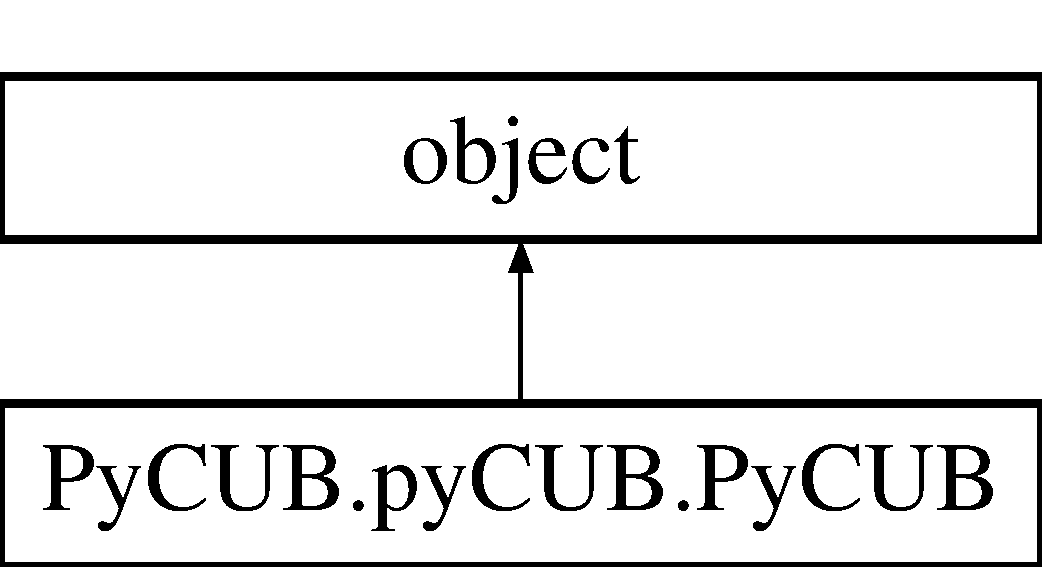
\includegraphics[height=2.000000cm]{class_py_c_u_b_1_1py_c_u_b_1_1_py_c_u_b}
\end{center}
\end{figure}
\subsection*{Public Member Functions}
\begin{DoxyCompactItemize}
\item 
def \mbox{\hyperlink{class_py_c_u_b_1_1py_c_u_b_1_1_py_c_u_b_a0a8de5f32a03de2c681c0582d9998f03}{\+\_\+\+\_\+init\+\_\+\+\_\+}} (self, species=\{\}, \+\_\+is\+\_\+saved=False, \+\_\+is\+\_\+loaded=False, working\+\_\+homoset=None, all\+\_\+homoset=None, session=\textquotesingle{}session1\textquotesingle{})
\begin{DoxyCompactList}\small\item\em will initialize the object with the different values you might have from another project \end{DoxyCompactList}\item 
def \mbox{\hyperlink{class_py_c_u_b_1_1py_c_u_b_1_1_py_c_u_b_ae06a2843c0718f86396ee255dfc6ae6f}{get\+Homologylist}} (self, species=\textquotesingle{}saccharomyces\+\_\+cerevisiae\textquotesingle{}, kingdom=\textquotesingle{}fungi\textquotesingle{})
\begin{DoxyCompactList}\small\item\em A function to retrieve the homologies directly from a given species. \end{DoxyCompactList}\item 
def \mbox{\hyperlink{class_py_c_u_b_1_1py_c_u_b_1_1_py_c_u_b_ac4d231f47432a18f84da1cef8673b50b}{get\+\_\+data}} (self, From=\textquotesingle{}yun\textquotesingle{}, homonames=None, kingdom=\textquotesingle{}fungi\textquotesingle{}, sequence=\textquotesingle{}cdna\textquotesingle{}, additional=\textquotesingle{}type=orthologues\textquotesingle{}, saveonfiles=False, normalized=True, setnans=False, by=\char`\"{}entropy\char`\"{}, using=\char`\"{}normal\char`\"{}, t\+R\+NA=True, get\+C\+AI=True, first=20, inpar=True)
\begin{DoxyCompactList}\small\item\em Download the data from somewhere on the web (Ensembl, Yun(with links)) \end{DoxyCompactList}\item 
def \mbox{\hyperlink{class_py_c_u_b_1_1py_c_u_b_1_1_py_c_u_b_ae561ba39b9c3919a83b51944f155e4a4}{get\+\_\+metadata\+\_\+\+Ensembl}} (self, kingdoms)
\begin{DoxyCompactList}\small\item\em download it and put it where it belongs in the Espece object \end{DoxyCompactList}\item 
def \mbox{\hyperlink{class_py_c_u_b_1_1py_c_u_b_1_1_py_c_u_b_a1ff011ae5b64518d60bedcf1b98314ef}{get\+\_\+mymetadata}} (self, From=\textquotesingle{}jerem\textquotesingle{}, inpar=True)
\begin{DoxyCompactList}\small\item\em Go ahead and design your own metadata retrieval here. \end{DoxyCompactList}\item 
def \mbox{\hyperlink{class_py_c_u_b_1_1py_c_u_b_1_1_py_c_u_b_acd80f084f6671584c42542813874cd02}{import\+\_\+metadata\+Tobias}} (self)
\begin{DoxyCompactList}\small\item\em will import the metadata obtained from tobias for the fungi species affiliated to cerevisiae to each species for further diagnostics. \end{DoxyCompactList}\item 
def \mbox{\hyperlink{class_py_c_u_b_1_1py_c_u_b_1_1_py_c_u_b_ab471e823b0eba23af5a5322008ec09da}{load}} (self, session=None, All=False, filename=\textquotesingle{}first500\textquotesingle{}, From=None, by=\textquotesingle{}entropy\textquotesingle{}, t\+R\+NA=True, inpar=True)
\begin{DoxyCompactList}\small\item\em Get the data that is already present on a filename. \end{DoxyCompactList}\item 
def \mbox{\hyperlink{class_py_c_u_b_1_1py_c_u_b_1_1_py_c_u_b_a16a1ab6be5dddcedf94852088936c1f2}{loadmore}} (self, filename=\textquotesingle{}first500\textquotesingle{}, by=\textquotesingle{}entropy\+Location\textquotesingle{})
\begin{DoxyCompactList}\small\item\em Get the data that is already present on a filename when you already have data. \end{DoxyCompactList}\item 
def \mbox{\hyperlink{class_py_c_u_b_1_1py_c_u_b_1_1_py_c_u_b_a477c55065989b10bce8389c5edaf3322}{save}} (self, name, save\+\_\+workspace=True, save\+\_\+homo=True, add\+\_\+homosets=\{\}, cmdlinetozip=\char`\"{}gzip\char`\"{})
\begin{DoxyCompactList}\small\item\em call to save your work. \end{DoxyCompactList}\item 
def \mbox{\hyperlink{class_py_c_u_b_1_1py_c_u_b_1_1_py_c_u_b_a1916ef696d74af1028a2aeff643727db}{get\+\_\+working\+\_\+homoset}} (self, clusternb=None, species=None, homologies=None, cleanhomo=None)
\begin{DoxyCompactList}\small\item\em create a subset of all\+\_\+homoset on which you would like to do further computation \end{DoxyCompactList}\item 
def \mbox{\hyperlink{class_py_c_u_b_1_1py_c_u_b_1_1_py_c_u_b_a9fab964d44e03b46d330b3754f5c39fb}{get\+\_\+subset}} (self, homoset, withcopy=False, clusternb=None, species=None, homologies=None)
\begin{DoxyCompactList}\small\item\em either changes or returns a subset of the provided homoset \end{DoxyCompactList}\item 
def \mbox{\hyperlink{class_py_c_u_b_1_1py_c_u_b_1_1_py_c_u_b_a53b60adfafbe019421d010c5fed04f5c}{get\+\_\+full\+\_\+genomes}} (self, kingdom=\textquotesingle{}fungi\textquotesingle{}, seq=\textquotesingle{}cds\textquotesingle{}, avg=True, by=\char`\"{}entropy\char`\"{}, normalized=False)
\begin{DoxyCompactList}\small\item\em go trought all full genome fasta files in the ftp server of ensemblgenomes and \end{DoxyCompactList}\item 
def \mbox{\hyperlink{class_py_c_u_b_1_1py_c_u_b_1_1_py_c_u_b_a4e9a2d43aacfc8d2fb1610140f2439f2}{get\+\_\+taxons}} (self)
\begin{DoxyCompactList}\small\item\em find the taxons of each referenced species (see Py\+C\+U\+B.\+Espece.\+gettaxons()) \end{DoxyCompactList}\item 
def \mbox{\hyperlink{class_py_c_u_b_1_1py_c_u_b_1_1_py_c_u_b_af0d7bed125f4437bea6b8051f9922c1d}{get\+\_\+evolutionary\+\_\+distance}} (self, display\+\_\+tree=False, size=40)
\begin{DoxyCompactList}\small\item\em uses metadata of the ancestry tree and computes a theoretical evolutionary distance matrix between each species \end{DoxyCompactList}\item 
def \mbox{\hyperlink{class_py_c_u_b_1_1py_c_u_b_1_1_py_c_u_b_a40a742a1a05fc21c7bced2c75fb93fc6}{create\+Ref\+C\+AI}} (self, speciestocompare=\textquotesingle{}saccharomyces\+\_\+cerevisiae\textquotesingle{}, kingdom=\textquotesingle{}fungi\textquotesingle{}, first=20)
\begin{DoxyCompactList}\small\item\em do a compute C\+AI \end{DoxyCompactList}\item 
def \mbox{\hyperlink{class_py_c_u_b_1_1py_c_u_b_1_1_py_c_u_b_af3e280c265200f13946e4bdcb4cd9dd0}{speciestable}} (self)
\begin{DoxyCompactList}\small\item\em a copy of the utils.\+speciestable \end{DoxyCompactList}\item 
def \mbox{\hyperlink{class_py_c_u_b_1_1py_c_u_b_1_1_py_c_u_b_a2ea40ac1dd5b4ad8847ec12c867d457f}{phylo\+\_\+distances}} (self)
\begin{DoxyCompactList}\small\item\em a copy of the phylodistances dataframe see (\mbox{\hyperlink{class_py_c_u_b_1_1py_c_u_b_1_1_py_c_u_b_af0d7bed125f4437bea6b8051f9922c1d}{get\+\_\+evolutionary\+\_\+distance()}}) \end{DoxyCompactList}\item 
def \mbox{\hyperlink{class_py_c_u_b_1_1py_c_u_b_1_1_py_c_u_b_a9526c0d10381daf5abc8ea120454e701}{compute\+\_\+averages}} (self, homoset)
\begin{DoxyCompactList}\small\item\em compute the average entropy \end{DoxyCompactList}\item 
def \mbox{\hyperlink{class_py_c_u_b_1_1py_c_u_b_1_1_py_c_u_b_ad7f24b316bc8c257719da20c0792ec01}{compare\+\_\+species}} (self, showvar=True, reducer=\textquotesingle{}tsne\textquotesingle{}, perplexity=40, eps=0.\+3, size=10)
\begin{DoxyCompactList}\small\item\em compare the species according to their mean C\+UB, \end{DoxyCompactList}\item 
\mbox{\Hypertarget{class_py_c_u_b_1_1py_c_u_b_1_1_py_c_u_b_af1cab3e8d69796c1a9a54a57a76228cd}\label{class_py_c_u_b_1_1py_c_u_b_1_1_py_c_u_b_af1cab3e8d69796c1a9a54a57a76228cd}} 
def {\bfseries compute\+\_\+ages} (self, homoset, preserved=True, minpreserv=0.\+9, minsimi=0.\+85)
\item 
def \mbox{\hyperlink{class_py_c_u_b_1_1py_c_u_b_1_1_py_c_u_b_af37319783148fc8864d894b3e2f89078}{regress\+\_\+on\+\_\+species}} (self, without=\mbox{[}\char`\"{}\char`\"{}\mbox{]}, full=True, onlyhomo=False, perctrain=0.\+8, algo=\char`\"{}lasso\char`\"{}, eps=0.\+001, n\+\_\+alphas=100)
\begin{DoxyCompactList}\small\item\em Will fit a regression curve on the C\+UB values of the different species according to the metadatas available for each of them. \end{DoxyCompactList}\item 
def \mbox{\hyperlink{class_py_c_u_b_1_1py_c_u_b_1_1_py_c_u_b_ad350376cd68d4daacec78c694ed754c6}{compare\+\_\+homologies}} (self, homoset, homosapiens=False, mindistance=10, preserved=True, size=10, minpreserv=0.\+9, minsimi=0.\+9, showvar=True, eps=0.\+28, reducer=\textquotesingle{}tsne\textquotesingle{}, perplexity=40)
\begin{DoxyCompactList}\small\item\em finds for species with a common ancester separated by a pseudo phylogenetic distance X, \end{DoxyCompactList}\item 
def \mbox{\hyperlink{class_py_c_u_b_1_1py_c_u_b_1_1_py_c_u_b_a1b65efe7deb4ba5f65203c8be6fc7af2}{regress\+\_\+on\+\_\+genes}} (self, homoset, full=True, without=\mbox{[}\textquotesingle{}meanecai\textquotesingle{}, meancai, perctrain=0.\+8, algo=\char`\"{}lasso\char`\"{}, eps=0.\+001, n\+\_\+alphas=100)
\begin{DoxyCompactList}\small\item\em Will fit a regression curve on the C\+UB values of the different homologies according to the metadatas available for each of them. \end{DoxyCompactList}\item 
def \mbox{\hyperlink{class_py_c_u_b_1_1py_c_u_b_1_1_py_c_u_b_a06d83a29ac506b4a9422ef7e64eef0b0}{get\+Relation2\+G3\+DD}} (self, species\+\_\+name=\textquotesingle{}saccharomyces\+\_\+cerevisiae\textquotesingle{}, kingdom=\textquotesingle{}fungi\textquotesingle{}, intrachromosome=\char`\"{}utils/meta/3\+Dmodel/interactions\+\_\+\+Hind\+I\+I\+I\+\_\+fdr0.\+01\+\_\+intra\+\_\+cerevisiae.\+csv\char`\"{}, interchromose=\mbox{[}\char`\"{}utils/meta/3\+Dmodel/cerevisiae\+\_\+inter1.\+csv\char`\"{}, utils, meta, Dmodel, cerevisiae\+\_\+inter2, csv, utils, meta, Dmodel, cerevisiae\+\_\+inter3, csv, utils, meta, Dmodel, cerevisiae\+\_\+inter4, csv, utils, meta, Dmodel, cerevisiae\+\_\+inter5, csv, bins=2000, seq=\textquotesingle{}cds\textquotesingle{}, use=\textquotesingle{}diament2\textquotesingle{})
\begin{DoxyCompactList}\small\item\em \href{https://www.nature.com/articles/ncomms6876}{\tt https\+://www.\+nature.\+com/articles/ncomms6876} \end{DoxyCompactList}\item 
def \mbox{\hyperlink{class_py_c_u_b_1_1py_c_u_b_1_1_py_c_u_b_a4e13b55153bbe774e9203818f2b7f690}{plot\+\_\+distances}} (self, size=40)
\begin{DoxyCompactList}\small\item\em plot the phylogenetic distance matrix \end{DoxyCompactList}\item 
def \mbox{\hyperlink{class_py_c_u_b_1_1py_c_u_b_1_1_py_c_u_b_ac37364050a4ec9a7ddf3d6c1562e49a5}{loadspeciestable}} (self)
\begin{DoxyCompactList}\small\item\em short function to retrieve the speciestable from Disk \end{DoxyCompactList}\item 
def \mbox{\hyperlink{class_py_c_u_b_1_1py_c_u_b_1_1_py_c_u_b_a8249834e1d2f7d061ae06ffa5a1adc32}{savespeciestable}} (self)
\begin{DoxyCompactList}\small\item\em short function to put the speciestable on Disk \end{DoxyCompactList}\end{DoxyCompactItemize}
\subsection*{Public Attributes}
\begin{DoxyCompactItemize}
\item 
\mbox{\Hypertarget{class_py_c_u_b_1_1py_c_u_b_1_1_py_c_u_b_a60cc232d3d52f88fe8a80244b3fcddc8}\label{class_py_c_u_b_1_1py_c_u_b_1_1_py_c_u_b_a60cc232d3d52f88fe8a80244b3fcddc8}} 
{\bfseries species}
\item 
\mbox{\Hypertarget{class_py_c_u_b_1_1py_c_u_b_1_1_py_c_u_b_a91b69c31f346c4983b40c1525739cf16}\label{class_py_c_u_b_1_1py_c_u_b_1_1_py_c_u_b_a91b69c31f346c4983b40c1525739cf16}} 
{\bfseries homolist}
\item 
\mbox{\Hypertarget{class_py_c_u_b_1_1py_c_u_b_1_1_py_c_u_b_ab2fcbabe6d3870dbbaa0cfd11605b004}\label{class_py_c_u_b_1_1py_c_u_b_1_1_py_c_u_b_ab2fcbabe6d3870dbbaa0cfd11605b004}} 
{\bfseries pent}
\item 
\mbox{\Hypertarget{class_py_c_u_b_1_1py_c_u_b_1_1_py_c_u_b_a9f1b34d59aff65055117cde8a174a474}\label{class_py_c_u_b_1_1py_c_u_b_1_1_py_c_u_b_a9f1b34d59aff65055117cde8a174a474}} 
{\bfseries pcub}
\item 
\mbox{\Hypertarget{class_py_c_u_b_1_1py_c_u_b_1_1_py_c_u_b_a0081f01dedc28de7864a2424c6760546}\label{class_py_c_u_b_1_1py_c_u_b_1_1_py_c_u_b_a0081f01dedc28de7864a2424c6760546}} 
{\bfseries pcuf}
\end{DoxyCompactItemize}
\subsection*{Static Public Attributes}
\begin{DoxyCompactItemize}
\item 
\mbox{\Hypertarget{class_py_c_u_b_1_1py_c_u_b_1_1_py_c_u_b_a34f579da0a139dffa0a01c3a90e9ef8d}\label{class_py_c_u_b_1_1py_c_u_b_1_1_py_c_u_b_a34f579da0a139dffa0a01c3a90e9ef8d}} 
dictionary {\bfseries links}
\item 
\mbox{\Hypertarget{class_py_c_u_b_1_1py_c_u_b_1_1_py_c_u_b_a39f174e37479c070657a4e9e710a53ca}\label{class_py_c_u_b_1_1py_c_u_b_1_1_py_c_u_b_a39f174e37479c070657a4e9e710a53ca}} 
dictionary {\bfseries species} = \{\}
\item 
\mbox{\Hypertarget{class_py_c_u_b_1_1py_c_u_b_1_1_py_c_u_b_ad3b3799416b15243c9027230dcd68482}\label{class_py_c_u_b_1_1py_c_u_b_1_1_py_c_u_b_ad3b3799416b15243c9027230dcd68482}} 
{\bfseries working\+\_\+homoset} = None
\item 
\mbox{\Hypertarget{class_py_c_u_b_1_1py_c_u_b_1_1_py_c_u_b_a5e68f8b0897b4e75b69abd6f1ac1beed}\label{class_py_c_u_b_1_1py_c_u_b_1_1_py_c_u_b_a5e68f8b0897b4e75b69abd6f1ac1beed}} 
{\bfseries all\+\_\+homoset} = None
\item 
\mbox{\Hypertarget{class_py_c_u_b_1_1py_c_u_b_1_1_py_c_u_b_a24fdc39b781fc1974625810704bd8140}\label{class_py_c_u_b_1_1py_c_u_b_1_1_py_c_u_b_a24fdc39b781fc1974625810704bd8140}} 
{\bfseries session} = None
\item 
\mbox{\Hypertarget{class_py_c_u_b_1_1py_c_u_b_1_1_py_c_u_b_abf0e792c29eb4ea90049ca996cad0022}\label{class_py_c_u_b_1_1py_c_u_b_1_1_py_c_u_b_abf0e792c29eb4ea90049ca996cad0022}} 
{\bfseries coeffgenes} = None
\item 
\mbox{\Hypertarget{class_py_c_u_b_1_1py_c_u_b_1_1_py_c_u_b_a70eae30eb6f055c7955969ec573a3f23}\label{class_py_c_u_b_1_1py_c_u_b_1_1_py_c_u_b_a70eae30eb6f055c7955969ec573a3f23}} 
{\bfseries scoregenes} = None
\item 
\mbox{\Hypertarget{class_py_c_u_b_1_1py_c_u_b_1_1_py_c_u_b_acbae28b1a15a26eedfa82aed4c8ae24f}\label{class_py_c_u_b_1_1py_c_u_b_1_1_py_c_u_b_acbae28b1a15a26eedfa82aed4c8ae24f}} 
{\bfseries scorespecies} = None
\item 
\mbox{\Hypertarget{class_py_c_u_b_1_1py_c_u_b_1_1_py_c_u_b_a37440d3a799d825552f477fc4a44c54f}\label{class_py_c_u_b_1_1py_c_u_b_1_1_py_c_u_b_a37440d3a799d825552f477fc4a44c54f}} 
{\bfseries coeffspecies} = None
\end{DoxyCompactItemize}
\subsection*{Private Member Functions}
\begin{DoxyCompactItemize}
\item 
def \mbox{\hyperlink{class_py_c_u_b_1_1py_c_u_b_1_1_py_c_u_b_acf1d1899b90f65a22eef8bc93b1735ab}{\+\_\+dictify}} (self, save\+\_\+workspace, save\+\_\+homo, add\+\_\+homosets)
\begin{DoxyCompactList}\small\item\em Used by the saving function. \end{DoxyCompactList}\item 
def \mbox{\hyperlink{class_py_c_u_b_1_1py_c_u_b_1_1_py_c_u_b_a8f60d259562234b7872cdc9cef03ce75}{\+\_\+undictify}} (self, data)
\begin{DoxyCompactList}\small\item\em same function but to retransform everything \end{DoxyCompactList}\end{DoxyCompactItemize}
\subsection*{Private Attributes}
\begin{DoxyCompactItemize}
\item 
\mbox{\Hypertarget{class_py_c_u_b_1_1py_c_u_b_1_1_py_c_u_b_aeb1012203f7072dafb43d297f76a438e}\label{class_py_c_u_b_1_1py_c_u_b_1_1_py_c_u_b_aeb1012203f7072dafb43d297f76a438e}} 
{\bfseries \+\_\+is\+\_\+saved}
\item 
\mbox{\Hypertarget{class_py_c_u_b_1_1py_c_u_b_1_1_py_c_u_b_a1cfa3e77ee07be4e8f1dd233fc97fea3}\label{class_py_c_u_b_1_1py_c_u_b_1_1_py_c_u_b_a1cfa3e77ee07be4e8f1dd233fc97fea3}} 
{\bfseries \+\_\+is\+\_\+loaded}
\end{DoxyCompactItemize}
\subsection*{Static Private Attributes}
\begin{DoxyCompactItemize}
\item 
\mbox{\Hypertarget{class_py_c_u_b_1_1py_c_u_b_1_1_py_c_u_b_aeb1012203f7072dafb43d297f76a438e}\label{class_py_c_u_b_1_1py_c_u_b_1_1_py_c_u_b_aeb1012203f7072dafb43d297f76a438e}} 
bool {\bfseries \+\_\+is\+\_\+saved}
\end{DoxyCompactItemize}


\subsection{Detailed Description}
\mbox{\hyperlink{class_py_c_u_b_1_1py_c_u_b_1_1_py_c_u_b}{Py\+C\+UB}} is the main object of the project that allows the user to access most of the functions. 

When using it, please follow the documentation and examples on notebooks thought you can still use it as you please and use some of the nice tricks provided here and in python


\begin{DoxyParams}{Parameters}
{\em species} & dictionary of Espece objects from the name of the species. (see espece.\+py) \\
\hline
{\em working\+\_\+homoset} & Py\+C\+U\+B.\+homoset object that stores a subset of the homologies you want to work on all\+\_\+homoset Py\+C\+U\+B.\+homoset that stores the all the homologies \\
\hline
{\em session} & str the session name you want to use (will appear in the savings for example \\
\hline
{\em \+\_\+is\+\_\+saved} & bool trivial system only boolean \\
\hline
{\em links} & dict of all the links readily available in \mbox{\hyperlink{class_py_c_u_b_1_1py_c_u_b_1_1_py_c_u_b}{Py\+C\+UB}}. for the project of Jeremie K\+A\+L\+F\+ON please use whatever datasets you may find usefull (you can also download from Ensembl)\\
\hline
{\em coeffgenes} & np.\+array regressing values for each attributes \\
\hline
{\em scoregenes} & the score of the regressor \\
\hline
{\em scorespecies} & the score of the regressor \\
\hline
{\em coeffspecies} & np.\+array regressing values for each attributes \\
\hline
\end{DoxyParams}


\subsection{Constructor \& Destructor Documentation}
\mbox{\Hypertarget{class_py_c_u_b_1_1py_c_u_b_1_1_py_c_u_b_a0a8de5f32a03de2c681c0582d9998f03}\label{class_py_c_u_b_1_1py_c_u_b_1_1_py_c_u_b_a0a8de5f32a03de2c681c0582d9998f03}} 
\index{Py\+C\+U\+B\+::py\+C\+U\+B\+::\+Py\+C\+UB@{Py\+C\+U\+B\+::py\+C\+U\+B\+::\+Py\+C\+UB}!\+\_\+\+\_\+init\+\_\+\+\_\+@{\+\_\+\+\_\+init\+\_\+\+\_\+}}
\index{\+\_\+\+\_\+init\+\_\+\+\_\+@{\+\_\+\+\_\+init\+\_\+\+\_\+}!Py\+C\+U\+B\+::py\+C\+U\+B\+::\+Py\+C\+UB@{Py\+C\+U\+B\+::py\+C\+U\+B\+::\+Py\+C\+UB}}
\subsubsection{\texorpdfstring{\+\_\+\+\_\+init\+\_\+\+\_\+()}{\_\_init\_\_()}}
{\footnotesize\ttfamily def Py\+C\+U\+B.\+py\+C\+U\+B.\+Py\+C\+U\+B.\+\_\+\+\_\+init\+\_\+\+\_\+ (\begin{DoxyParamCaption}\item[{}]{self,  }\item[{}]{species = {\ttfamily \{\}},  }\item[{}]{\+\_\+is\+\_\+saved = {\ttfamily False},  }\item[{}]{\+\_\+is\+\_\+loaded = {\ttfamily False},  }\item[{}]{working\+\_\+homoset = {\ttfamily None},  }\item[{}]{all\+\_\+homoset = {\ttfamily None},  }\item[{}]{session = {\ttfamily \textquotesingle{}session1\textquotesingle{}} }\end{DoxyParamCaption})}



will initialize the object with the different values you might have from another project 


\begin{DoxyParams}{Parameters}
{\em species} & dictionary of Espece objects from the name of the species. (see espece.\+py) \\
\hline
{\em working\+\_\+homoset} & Py\+C\+U\+B.\+homoset object that stores a subset of the homologies you want to work on all\+\_\+homoset Py\+C\+U\+B.\+homoset that stores the all the homologies \\
\hline
{\em session} & str the session name you want to use (will appear in the savings for example \\
\hline
{\em \+\_\+is\+\_\+saved} & bool trivial system only boolean \\
\hline
\end{DoxyParams}


\subsection{Member Function Documentation}
\mbox{\Hypertarget{class_py_c_u_b_1_1py_c_u_b_1_1_py_c_u_b_acf1d1899b90f65a22eef8bc93b1735ab}\label{class_py_c_u_b_1_1py_c_u_b_1_1_py_c_u_b_acf1d1899b90f65a22eef8bc93b1735ab}} 
\index{Py\+C\+U\+B\+::py\+C\+U\+B\+::\+Py\+C\+UB@{Py\+C\+U\+B\+::py\+C\+U\+B\+::\+Py\+C\+UB}!\+\_\+dictify@{\+\_\+dictify}}
\index{\+\_\+dictify@{\+\_\+dictify}!Py\+C\+U\+B\+::py\+C\+U\+B\+::\+Py\+C\+UB@{Py\+C\+U\+B\+::py\+C\+U\+B\+::\+Py\+C\+UB}}
\subsubsection{\texorpdfstring{\+\_\+dictify()}{\_dictify()}}
{\footnotesize\ttfamily def Py\+C\+U\+B.\+py\+C\+U\+B.\+Py\+C\+U\+B.\+\_\+dictify (\begin{DoxyParamCaption}\item[{}]{self,  }\item[{}]{save\+\_\+workspace,  }\item[{}]{save\+\_\+homo,  }\item[{}]{add\+\_\+homosets }\end{DoxyParamCaption})\hspace{0.3cm}{\ttfamily [private]}}



Used by the saving function. 

transform the workspace object into a dictionary that can be json serializable \begin{DoxyVerb}   adding some params because else the object may be too big
\end{DoxyVerb}



\begin{DoxyParams}{Parameters}
{\em save\+\_\+workspace} & bool to save working\+\_\+homoset \\
\hline
{\em save\+\_\+homo} & bool to save all\+\_\+homoset \\
\hline
{\em ass\+\_\+homosets} & Py\+C\+U\+B.\+homoset instances to add to this dict\\
\hline
\end{DoxyParams}
\begin{DoxyParagraph}{Return}
A dict holding every element to be jsonized 
\end{DoxyParagraph}


Referenced by Py\+C\+U\+B.\+py\+C\+U\+B.\+Py\+C\+U\+B.\+plot\+\_\+distances(), and Py\+C\+U\+B.\+py\+C\+U\+B.\+Py\+C\+U\+B.\+save().

\mbox{\Hypertarget{class_py_c_u_b_1_1py_c_u_b_1_1_py_c_u_b_a8f60d259562234b7872cdc9cef03ce75}\label{class_py_c_u_b_1_1py_c_u_b_1_1_py_c_u_b_a8f60d259562234b7872cdc9cef03ce75}} 
\index{Py\+C\+U\+B\+::py\+C\+U\+B\+::\+Py\+C\+UB@{Py\+C\+U\+B\+::py\+C\+U\+B\+::\+Py\+C\+UB}!\+\_\+undictify@{\+\_\+undictify}}
\index{\+\_\+undictify@{\+\_\+undictify}!Py\+C\+U\+B\+::py\+C\+U\+B\+::\+Py\+C\+UB@{Py\+C\+U\+B\+::py\+C\+U\+B\+::\+Py\+C\+UB}}
\subsubsection{\texorpdfstring{\+\_\+undictify()}{\_undictify()}}
{\footnotesize\ttfamily def Py\+C\+U\+B.\+py\+C\+U\+B.\+Py\+C\+U\+B.\+\_\+undictify (\begin{DoxyParamCaption}\item[{}]{self,  }\item[{}]{data }\end{DoxyParamCaption})\hspace{0.3cm}{\ttfamily [private]}}



same function but to retransform everything 

Here we don\textquotesingle{}t use other classes undictify functions but we just recreate them by passing it to their init methods which is clearer.


\begin{DoxyParams}{Parameters}
{\em data} & dict to undictify into the workspace object\\
\hline
\end{DoxyParams}
\begin{DoxyReturn}{Returns}
Other Py\+C\+U\+B.\+homosets that would have been saved as add\+\_\+homosets 
\end{DoxyReturn}


Referenced by Py\+C\+U\+B.\+py\+C\+U\+B.\+Py\+C\+U\+B.\+\_\+dictify(), and Py\+C\+U\+B.\+py\+C\+U\+B.\+Py\+C\+U\+B.\+load().

\mbox{\Hypertarget{class_py_c_u_b_1_1py_c_u_b_1_1_py_c_u_b_ad350376cd68d4daacec78c694ed754c6}\label{class_py_c_u_b_1_1py_c_u_b_1_1_py_c_u_b_ad350376cd68d4daacec78c694ed754c6}} 
\index{Py\+C\+U\+B\+::py\+C\+U\+B\+::\+Py\+C\+UB@{Py\+C\+U\+B\+::py\+C\+U\+B\+::\+Py\+C\+UB}!compare\+\_\+homologies@{compare\+\_\+homologies}}
\index{compare\+\_\+homologies@{compare\+\_\+homologies}!Py\+C\+U\+B\+::py\+C\+U\+B\+::\+Py\+C\+UB@{Py\+C\+U\+B\+::py\+C\+U\+B\+::\+Py\+C\+UB}}
\subsubsection{\texorpdfstring{compare\+\_\+homologies()}{compare\_homologies()}}
{\footnotesize\ttfamily def Py\+C\+U\+B.\+py\+C\+U\+B.\+Py\+C\+U\+B.\+compare\+\_\+homologies (\begin{DoxyParamCaption}\item[{}]{self,  }\item[{}]{homoset,  }\item[{}]{homosapiens = {\ttfamily False},  }\item[{}]{mindistance = {\ttfamily 10},  }\item[{}]{preserved = {\ttfamily True},  }\item[{}]{size = {\ttfamily 10},  }\item[{}]{minpreserv = {\ttfamily 0.9},  }\item[{}]{minsimi = {\ttfamily 0.9},  }\item[{}]{showvar = {\ttfamily True},  }\item[{}]{eps = {\ttfamily 0.28},  }\item[{}]{reducer = {\ttfamily \textquotesingle{}tsne\textquotesingle{}},  }\item[{}]{perplexity = {\ttfamily 40} }\end{DoxyParamCaption})}



finds for species with a common ancester separated by a pseudo phylogenetic distance X, 

genes/functions that are novel to only a subset. plot the two with their differences the differences between the two also considers an homology as highly preserved if it is shared amongst most of the species and if the average similarity score is high amongst this homology. also shows if there is a relationship between the number of amino acids the sequence does not encode for and the codon usage bias We could have used the sequence dating of ensembl but it only works for homo sapiens for now maybe use it for homosapiens later


\begin{DoxyParams}{Parameters}
{\em homosapiens} & bool to true if we should use homosapiens dataset on gene dates \\
\hline
{\em mindistance} & int the minimal phylogenetic distance between in average in this homology to consider it highly conserved \\
\hline
{\em preserved} & bool to true if we should find highly preserved genes or not \\
\hline
{\em size} & the average size of the datapoints in the pointcloud representation of this dataset \\
\hline
{\em minpreserv} & float minimal percentage of homologous species that have this homology \\
\hline
{\em minsimi} & float minimal avg similarity between genes to consider them highly preserved \\
\hline
{\em showvar} & bool to true, show the mean variance in C\+UB values accros this homology as a variation in dot sizes \\
\hline
{\em eps} & float the hyperparamter of the clustering algorithm applied to this dataset \\
\hline
{\em homoset} & Py\+C\+U\+B.\+homoset the homoset to use \\
\hline
{\em reducer} & str the reducer to use \textquotesingle{}tsne\textquotesingle{} or \textquotesingle{}P\+CA\textquotesingle{} \\
\hline
{\em perplexity} & int the perplexity hyperparam for t\+S\+NE\\
\hline
\end{DoxyParams}

\begin{DoxyExceptions}{Exceptions}
{\em Unbound\+Local\+Error} & \char`\"{}you need to compute the averages of the all\+\_\+homoset. use Py\+C\+U\+B.\+compute\+\_\+averages(homoset)\char`\"{} \\
\hline
\end{DoxyExceptions}


Referenced by Py\+C\+U\+B.\+py\+C\+U\+B.\+Py\+C\+U\+B.\+regress\+\_\+on\+\_\+species().

\mbox{\Hypertarget{class_py_c_u_b_1_1py_c_u_b_1_1_py_c_u_b_ad7f24b316bc8c257719da20c0792ec01}\label{class_py_c_u_b_1_1py_c_u_b_1_1_py_c_u_b_ad7f24b316bc8c257719da20c0792ec01}} 
\index{Py\+C\+U\+B\+::py\+C\+U\+B\+::\+Py\+C\+UB@{Py\+C\+U\+B\+::py\+C\+U\+B\+::\+Py\+C\+UB}!compare\+\_\+species@{compare\+\_\+species}}
\index{compare\+\_\+species@{compare\+\_\+species}!Py\+C\+U\+B\+::py\+C\+U\+B\+::\+Py\+C\+UB@{Py\+C\+U\+B\+::py\+C\+U\+B\+::\+Py\+C\+UB}}
\subsubsection{\texorpdfstring{compare\+\_\+species()}{compare\_species()}}
{\footnotesize\ttfamily def Py\+C\+U\+B.\+py\+C\+U\+B.\+Py\+C\+U\+B.\+compare\+\_\+species (\begin{DoxyParamCaption}\item[{}]{self,  }\item[{}]{showvar = {\ttfamily True},  }\item[{}]{reducer = {\ttfamily \textquotesingle{}tsne\textquotesingle{}},  }\item[{}]{perplexity = {\ttfamily 40},  }\item[{}]{eps = {\ttfamily 0.3},  }\item[{}]{size = {\ttfamily 10} }\end{DoxyParamCaption})}



compare the species according to their mean C\+UB, 

plot the mean C\+UB to their full C\+UB, to their t\+R\+NA copy numbers, to the euclidean distance of their C\+UB to the one of their phylogenetic matrix. in this plot, the mean entropy value is plotted as a regular homology plot but each dot is a species thus we can compare them together, moreover, the size of the dots informs oneself of the variance in entropy per species. the color intensity informs on how much this is close to what is given by the t\+R\+NA values. (additional information such as name of the species, number of t\+R\+NA values,metadata and the point from its t\+R\+NA value is plotted when hovering the dot) then we can also compare the mean of homologies or else, the full entropy of the cdna sequence per species is also computed the euclidean distance amongst the species for the full entropy to see if a difference can be linked to some evolutionary for one codon


\begin{DoxyParams}{Parameters}
{\em size} & the average size of the datapoints in the pointcloud representation of this dataset \\
\hline
{\em showvar} & bool to true, show the mean variance in C\+UB values accros this homology as a variation in dot sizes \\
\hline
{\em eps} & float the hyperparamter of the clustering algorithm applied to this dataset \\
\hline
{\em homoset} & Py\+C\+U\+B.\+homoset the homoset to use \\
\hline
{\em reducer} & str the reducer to use \textquotesingle{}tsne\textquotesingle{} or \textquotesingle{}P\+CA\textquotesingle{} \\
\hline
{\em perplexity} & int the perplexity hyperparam for t\+S\+NE\\
\hline
\end{DoxyParams}

\begin{DoxyExceptions}{Exceptions}
{\em Unbound\+Local\+Error} & \char`\"{}you need to compute the averages of the all\+\_\+homoset. use Py\+C\+U\+B.\+compute\+\_\+averages(homoset)\char`\"{} \\
\hline
{\em Unbound\+Local\+Error} & \char`\"{}you have to compute t\+R\+N\+A values, use Py\+C\+U\+B.\+get\+\_\+t\+R\+N\+Acopy()\char`\"{} \\
\hline
{\em Attribute\+Error} & \char`\"{}try avg or full\char`\"{} \\
\hline
\end{DoxyExceptions}


Referenced by Py\+C\+U\+B.\+py\+C\+U\+B.\+Py\+C\+U\+B.\+compute\+\_\+averages().

\mbox{\Hypertarget{class_py_c_u_b_1_1py_c_u_b_1_1_py_c_u_b_a9526c0d10381daf5abc8ea120454e701}\label{class_py_c_u_b_1_1py_c_u_b_1_1_py_c_u_b_a9526c0d10381daf5abc8ea120454e701}} 
\index{Py\+C\+U\+B\+::py\+C\+U\+B\+::\+Py\+C\+UB@{Py\+C\+U\+B\+::py\+C\+U\+B\+::\+Py\+C\+UB}!compute\+\_\+averages@{compute\+\_\+averages}}
\index{compute\+\_\+averages@{compute\+\_\+averages}!Py\+C\+U\+B\+::py\+C\+U\+B\+::\+Py\+C\+UB@{Py\+C\+U\+B\+::py\+C\+U\+B\+::\+Py\+C\+UB}}
\subsubsection{\texorpdfstring{compute\+\_\+averages()}{compute\_averages()}}
{\footnotesize\ttfamily def Py\+C\+U\+B.\+py\+C\+U\+B.\+Py\+C\+U\+B.\+compute\+\_\+averages (\begin{DoxyParamCaption}\item[{}]{self,  }\item[{}]{homoset }\end{DoxyParamCaption})}



compute the average entropy 

Will add species related averages gotten from this homoset in the species container, and in the homoset everytime you compute averages from a set, they will get erased !


\begin{DoxyParams}{Parameters}
{\em homoset} & Py\+C\+U\+B.\+homoset from which to compute the averages \\
\hline
\end{DoxyParams}


Referenced by Py\+C\+U\+B.\+py\+C\+U\+B.\+Py\+C\+U\+B.\+speciestable().

\mbox{\Hypertarget{class_py_c_u_b_1_1py_c_u_b_1_1_py_c_u_b_a40a742a1a05fc21c7bced2c75fb93fc6}\label{class_py_c_u_b_1_1py_c_u_b_1_1_py_c_u_b_a40a742a1a05fc21c7bced2c75fb93fc6}} 
\index{Py\+C\+U\+B\+::py\+C\+U\+B\+::\+Py\+C\+UB@{Py\+C\+U\+B\+::py\+C\+U\+B\+::\+Py\+C\+UB}!create\+Ref\+C\+AI@{create\+Ref\+C\+AI}}
\index{create\+Ref\+C\+AI@{create\+Ref\+C\+AI}!Py\+C\+U\+B\+::py\+C\+U\+B\+::\+Py\+C\+UB@{Py\+C\+U\+B\+::py\+C\+U\+B\+::\+Py\+C\+UB}}
\subsubsection{\texorpdfstring{create\+Ref\+C\+A\+I()}{createRefCAI()}}
{\footnotesize\ttfamily def Py\+C\+U\+B.\+py\+C\+U\+B.\+Py\+C\+U\+B.\+create\+Ref\+C\+AI (\begin{DoxyParamCaption}\item[{}]{self,  }\item[{}]{speciestocompare = {\ttfamily \textquotesingle{}saccharomyces\+\_\+cerevisiae\textquotesingle{}},  }\item[{}]{kingdom = {\ttfamily \textquotesingle{}fungi\textquotesingle{}},  }\item[{}]{first = {\ttfamily 20} }\end{DoxyParamCaption})}



do a compute C\+AI 

where we get Tobias\textquotesingle{} data to find highly expressed genes and use them to compute codon frequency for the reference set and use it to compute the C\+AI and mean C\+AI for each ho mology.


\begin{DoxyParams}{Parameters}
{\em speciestocompare} & str the name of the species to retrieve the genes from \\
\hline
{\em kingdom} & str the kingdom where we can find it \\
\hline
{\em first} & the number of highly expressed genes to retrieve \\
\hline
\end{DoxyParams}


Referenced by Py\+C\+U\+B.\+py\+C\+U\+B.\+Py\+C\+U\+B.\+get\+\_\+data(), and Py\+C\+U\+B.\+py\+C\+U\+B.\+Py\+C\+U\+B.\+get\+\_\+evolutionary\+\_\+distance().

\mbox{\Hypertarget{class_py_c_u_b_1_1py_c_u_b_1_1_py_c_u_b_ac4d231f47432a18f84da1cef8673b50b}\label{class_py_c_u_b_1_1py_c_u_b_1_1_py_c_u_b_ac4d231f47432a18f84da1cef8673b50b}} 
\index{Py\+C\+U\+B\+::py\+C\+U\+B\+::\+Py\+C\+UB@{Py\+C\+U\+B\+::py\+C\+U\+B\+::\+Py\+C\+UB}!get\+\_\+data@{get\+\_\+data}}
\index{get\+\_\+data@{get\+\_\+data}!Py\+C\+U\+B\+::py\+C\+U\+B\+::\+Py\+C\+UB@{Py\+C\+U\+B\+::py\+C\+U\+B\+::\+Py\+C\+UB}}
\subsubsection{\texorpdfstring{get\+\_\+data()}{get\_data()}}
{\footnotesize\ttfamily def Py\+C\+U\+B.\+py\+C\+U\+B.\+Py\+C\+U\+B.\+get\+\_\+data (\begin{DoxyParamCaption}\item[{}]{self,  }\item[{}]{From = {\ttfamily \textquotesingle{}yun\textquotesingle{}},  }\item[{}]{homonames = {\ttfamily None},  }\item[{}]{kingdom = {\ttfamily \textquotesingle{}fungi\textquotesingle{}},  }\item[{}]{sequence = {\ttfamily \textquotesingle{}cdna\textquotesingle{}},  }\item[{}]{additional = {\ttfamily \textquotesingle{}type=orthologues\textquotesingle{}},  }\item[{}]{saveonfiles = {\ttfamily False},  }\item[{}]{normalized = {\ttfamily True},  }\item[{}]{setnans = {\ttfamily False},  }\item[{}]{by = {\ttfamily \char`\"{}entropy\char`\"{}},  }\item[{}]{using = {\ttfamily \char`\"{}normal\char`\"{}},  }\item[{}]{t\+R\+NA = {\ttfamily True},  }\item[{}]{get\+C\+AI = {\ttfamily True},  }\item[{}]{first = {\ttfamily 20},  }\item[{}]{inpar = {\ttfamily True} }\end{DoxyParamCaption})}



Download the data from somewhere on the web (Ensembl, Yun(with links)) 

you can provide a lot of different values to scrape Ensembl\textquotesingle{}s datasets it will compute from ensembl to retrieve a similar dataset as what yun\textquotesingle{}s data is.


\begin{DoxyParams}{Parameters}
{\em From} & str flag \textquotesingle{}yun\textquotesingle{} or \textquotesingle{}ensembl\textquotesingle{}\+: \\
\hline
{\em homonames} & list\mbox{[}str\mbox{]} what particular homologies you want to scrap if \textquotesingle{}all\textquotesingle{} and you have used the \mbox{\hyperlink{class_py_c_u_b_1_1py_c_u_b_1_1_py_c_u_b_ae06a2843c0718f86396ee255dfc6ae6f}{get\+Homologylist()}} function, will get the homologies from there \\
\hline
{\em kingdom} & str same for kingdoms \\
\hline
{\em sequence} & str the type of sequences you want to use \\
\hline
{\em additional} & str additional information about the scrapping \\
\hline
{\em saveonfiles} & bool save the unprocessed data before populating working homoset \\
\hline
{\em normalized} & bool if you want the values to be normalized by the length of the codons (lengths are always saved) \\
\hline
{\em setnans} & bool if you want to save the nans as metadata \\
\hline
{\em by} & str flag \textquotesingle{}entropy\textquotesingle{}, \textquotesingle{}entropy\+Location\textquotesingle{} (entropy location), \textquotesingle{}frequency\textquotesingle{} \\
\hline
{\em using} & str flag \textquotesingle{}random\textquotesingle{} \textquotesingle{}normal\textquotesingle{} \textquotesingle{}permutation\textquotesingle{} \textquotesingle{}full\textquotesingle{} \\
\hline
{\em inpar} & bool or int for parallel computing and number of core \\
\hline
{\em t\+R\+NA} & bool whether or not to compute t\+R\+NA data \\
\hline
{\em get\+C\+AI} & bool flag to true to retrieve the C\+AI as well \\
\hline
{\em first} & int the first most expressed genes to compute the C\+AI ref statistics\\
\hline
\end{DoxyParams}

\begin{DoxyExceptions}{Exceptions}
{\em Attribute\+Error} & \char`\"{}you can\textquotesingle{}t compute codon frequency with Yun\textquotesingle{}s data...\char`\"{}, \textquotesingle{}not the right From\textquotesingle{} \\
\hline
{\em Unbound\+Local\+Error} & \char`\"{}you have to load the homologies first\char`\"{} \\
\hline
{\em Attribute\+Error} & \textquotesingle{}not the right From\textquotesingle{} \begin{DoxyVerb}   http://rest.ensemblgenomes.org/\end{DoxyVerb}
 \\
\hline
\end{DoxyExceptions}


Referenced by Py\+C\+U\+B.\+py\+C\+U\+B.\+Py\+C\+U\+B.\+get\+Homologylist().

\mbox{\Hypertarget{class_py_c_u_b_1_1py_c_u_b_1_1_py_c_u_b_af0d7bed125f4437bea6b8051f9922c1d}\label{class_py_c_u_b_1_1py_c_u_b_1_1_py_c_u_b_af0d7bed125f4437bea6b8051f9922c1d}} 
\index{Py\+C\+U\+B\+::py\+C\+U\+B\+::\+Py\+C\+UB@{Py\+C\+U\+B\+::py\+C\+U\+B\+::\+Py\+C\+UB}!get\+\_\+evolutionary\+\_\+distance@{get\+\_\+evolutionary\+\_\+distance}}
\index{get\+\_\+evolutionary\+\_\+distance@{get\+\_\+evolutionary\+\_\+distance}!Py\+C\+U\+B\+::py\+C\+U\+B\+::\+Py\+C\+UB@{Py\+C\+U\+B\+::py\+C\+U\+B\+::\+Py\+C\+UB}}
\subsubsection{\texorpdfstring{get\+\_\+evolutionary\+\_\+distance()}{get\_evolutionary\_distance()}}
{\footnotesize\ttfamily def Py\+C\+U\+B.\+py\+C\+U\+B.\+Py\+C\+U\+B.\+get\+\_\+evolutionary\+\_\+distance (\begin{DoxyParamCaption}\item[{}]{self,  }\item[{}]{display\+\_\+tree = {\ttfamily False},  }\item[{}]{size = {\ttfamily 40} }\end{DoxyParamCaption})}



uses metadata of the ancestry tree and computes a theoretical evolutionary distance matrix between each species 

can optionaly take any hierarchical evolutionary file between a group of species will populate utils.\+phylo\+\_\+distances with a pandas.\+df of the phylodistance and meandist with the average distance amongst species in the df, species are referenced by their taxon ids. you have to have taxons in your species. will also plot the distance matrix


\begin{DoxyParams}{Parameters}
{\em display\+\_\+tree} & bool to true to print the phylogenetic tree as a txt (may be quite big) \\
\hline
{\em size} & int the x size of the plot\\
\hline
\end{DoxyParams}

\begin{DoxyExceptions}{Exceptions}
{\em Environment\+Error} & \char`\"{}you need to have R installed to compute the distance\char`\"{} \\
\hline
\end{DoxyExceptions}


Referenced by Py\+C\+U\+B.\+py\+C\+U\+B.\+Py\+C\+U\+B.\+get\+\_\+taxons().

\mbox{\Hypertarget{class_py_c_u_b_1_1py_c_u_b_1_1_py_c_u_b_a53b60adfafbe019421d010c5fed04f5c}\label{class_py_c_u_b_1_1py_c_u_b_1_1_py_c_u_b_a53b60adfafbe019421d010c5fed04f5c}} 
\index{Py\+C\+U\+B\+::py\+C\+U\+B\+::\+Py\+C\+UB@{Py\+C\+U\+B\+::py\+C\+U\+B\+::\+Py\+C\+UB}!get\+\_\+full\+\_\+genomes@{get\+\_\+full\+\_\+genomes}}
\index{get\+\_\+full\+\_\+genomes@{get\+\_\+full\+\_\+genomes}!Py\+C\+U\+B\+::py\+C\+U\+B\+::\+Py\+C\+UB@{Py\+C\+U\+B\+::py\+C\+U\+B\+::\+Py\+C\+UB}}
\subsubsection{\texorpdfstring{get\+\_\+full\+\_\+genomes()}{get\_full\_genomes()}}
{\footnotesize\ttfamily def Py\+C\+U\+B.\+py\+C\+U\+B.\+Py\+C\+U\+B.\+get\+\_\+full\+\_\+genomes (\begin{DoxyParamCaption}\item[{}]{self,  }\item[{}]{kingdom = {\ttfamily \textquotesingle{}fungi\textquotesingle{}},  }\item[{}]{seq = {\ttfamily \textquotesingle{}cds\textquotesingle{}},  }\item[{}]{avg = {\ttfamily True},  }\item[{}]{by = {\ttfamily \char`\"{}entropy\char`\"{}},  }\item[{}]{normalized = {\ttfamily False} }\end{DoxyParamCaption})}



go trought all full genome fasta files in the ftp server of ensemblgenomes and 

download then parse them to get the full entropy of the genome. usefull for futher comparison steps. will populate the fullentropy, fullvarentropy, full\+G\+Ccount, var\+G\+Ccount of each species where the full sequence is known


\begin{DoxyParams}{Parameters}
{\em kingdom} & str flags the relevant kingdom of you current session \mbox{[}fungi,plants,bacteria, animals\mbox{]} \\
\hline
{\em seq} & str flags the type of sequence you consider the full genome is (coding or non coding or full) \mbox{[}cds, all, cda\mbox{]} \\
\hline
{\em avg} & bool to true if we average over each gene or get the full dna in one go. \\
\hline
{\em by} & str flags what type of computation should be done \mbox{[}entropy,frequency\mbox{]} \\
\hline
{\em normalized} & should we normalize the entorpy by length\\
\hline
\end{DoxyParams}

\begin{DoxyExceptions}{Exceptions}
{\em Memory\+Error} & \char`\"{}this sequence is too long to be computed ($>$ 1 billion bp)\char`\"{} \\
\hline
\end{DoxyExceptions}


Referenced by Py\+C\+U\+B.\+py\+C\+U\+B.\+Py\+C\+U\+B.\+get\+\_\+subset().

\mbox{\Hypertarget{class_py_c_u_b_1_1py_c_u_b_1_1_py_c_u_b_ae561ba39b9c3919a83b51944f155e4a4}\label{class_py_c_u_b_1_1py_c_u_b_1_1_py_c_u_b_ae561ba39b9c3919a83b51944f155e4a4}} 
\index{Py\+C\+U\+B\+::py\+C\+U\+B\+::\+Py\+C\+UB@{Py\+C\+U\+B\+::py\+C\+U\+B\+::\+Py\+C\+UB}!get\+\_\+metadata\+\_\+\+Ensembl@{get\+\_\+metadata\+\_\+\+Ensembl}}
\index{get\+\_\+metadata\+\_\+\+Ensembl@{get\+\_\+metadata\+\_\+\+Ensembl}!Py\+C\+U\+B\+::py\+C\+U\+B\+::\+Py\+C\+UB@{Py\+C\+U\+B\+::py\+C\+U\+B\+::\+Py\+C\+UB}}
\subsubsection{\texorpdfstring{get\+\_\+metadata\+\_\+\+Ensembl()}{get\_metadata\_Ensembl()}}
{\footnotesize\ttfamily def Py\+C\+U\+B.\+py\+C\+U\+B.\+Py\+C\+U\+B.\+get\+\_\+metadata\+\_\+\+Ensembl (\begin{DoxyParamCaption}\item[{}]{self,  }\item[{}]{kingdoms }\end{DoxyParamCaption})}



download it and put it where it belongs in the Espece object 

parse the server \href{https://fungi.ensembl.org/info/website/ftp/index.html}{\tt https\+://fungi.\+ensembl.\+org/info/website/ftp/index.\+html} will also get the metadata from the kingdoms that you are analysing


\begin{DoxyParams}{Parameters}
{\em kingdoms} & str flag the type of kingdoms you wanna have \textquotesingle{}fungi\textquotesingle{} \textquotesingle{}bacteria\textquotesingle{} \textquotesingle{}plants\textquotesingle{} \textquotesingle{}animals\textquotesingle{} \\
\hline
\end{DoxyParams}


Referenced by Py\+C\+U\+B.\+py\+C\+U\+B.\+Py\+C\+U\+B.\+get\+\_\+data().

\mbox{\Hypertarget{class_py_c_u_b_1_1py_c_u_b_1_1_py_c_u_b_a1ff011ae5b64518d60bedcf1b98314ef}\label{class_py_c_u_b_1_1py_c_u_b_1_1_py_c_u_b_a1ff011ae5b64518d60bedcf1b98314ef}} 
\index{Py\+C\+U\+B\+::py\+C\+U\+B\+::\+Py\+C\+UB@{Py\+C\+U\+B\+::py\+C\+U\+B\+::\+Py\+C\+UB}!get\+\_\+mymetadata@{get\+\_\+mymetadata}}
\index{get\+\_\+mymetadata@{get\+\_\+mymetadata}!Py\+C\+U\+B\+::py\+C\+U\+B\+::\+Py\+C\+UB@{Py\+C\+U\+B\+::py\+C\+U\+B\+::\+Py\+C\+UB}}
\subsubsection{\texorpdfstring{get\+\_\+mymetadata()}{get\_mymetadata()}}
{\footnotesize\ttfamily def Py\+C\+U\+B.\+py\+C\+U\+B.\+Py\+C\+U\+B.\+get\+\_\+mymetadata (\begin{DoxyParamCaption}\item[{}]{self,  }\item[{}]{From = {\ttfamily \textquotesingle{}jerem\textquotesingle{}},  }\item[{}]{inpar = {\ttfamily True} }\end{DoxyParamCaption})}



Go ahead and design your own metadata retrieval here. 

obviously you woud need to change some other functions. for me it is mean protein abundances in cerevisiae cells.


\begin{DoxyParams}{Parameters}
{\em From} & str flag designer of the function to load metadatas \\
\hline
{\em inpar} & bool for parallel processing \\
\hline
\end{DoxyParams}


Referenced by Py\+C\+U\+B.\+py\+C\+U\+B.\+Py\+C\+U\+B.\+get\+\_\+metadata\+\_\+\+Ensembl().

\mbox{\Hypertarget{class_py_c_u_b_1_1py_c_u_b_1_1_py_c_u_b_a9fab964d44e03b46d330b3754f5c39fb}\label{class_py_c_u_b_1_1py_c_u_b_1_1_py_c_u_b_a9fab964d44e03b46d330b3754f5c39fb}} 
\index{Py\+C\+U\+B\+::py\+C\+U\+B\+::\+Py\+C\+UB@{Py\+C\+U\+B\+::py\+C\+U\+B\+::\+Py\+C\+UB}!get\+\_\+subset@{get\+\_\+subset}}
\index{get\+\_\+subset@{get\+\_\+subset}!Py\+C\+U\+B\+::py\+C\+U\+B\+::\+Py\+C\+UB@{Py\+C\+U\+B\+::py\+C\+U\+B\+::\+Py\+C\+UB}}
\subsubsection{\texorpdfstring{get\+\_\+subset()}{get\_subset()}}
{\footnotesize\ttfamily def Py\+C\+U\+B.\+py\+C\+U\+B.\+Py\+C\+U\+B.\+get\+\_\+subset (\begin{DoxyParamCaption}\item[{}]{self,  }\item[{}]{homoset,  }\item[{}]{withcopy = {\ttfamily False},  }\item[{}]{clusternb = {\ttfamily None},  }\item[{}]{species = {\ttfamily None},  }\item[{}]{homologies = {\ttfamily None} }\end{DoxyParamCaption})}



either changes or returns a subset of the provided homoset 

To use once if you want to further refine a set of homologies


\begin{DoxyParams}{Parameters}
{\em homoset} & Py\+C\+U\+B.\+homoset to get a subset from \\
\hline
{\em withcopy} & bool to true if we don\textquotesingle{}t want to change the homoset object but create a copy from it \\
\hline
{\em clusternb} & int set the cluster of the group you want to get need to be between 1 and homogroupnb \\
\hline
{\em homologies} & list\mbox{[}str\mbox{]} the subset as a list or a tuple of int \\
\hline
{\em species} & list\mbox{[}the subset as a list, or a list of int\\
\hline
\end{DoxyParams}
\begin{DoxyReturn}{Returns}
a Homo\+Set object (see homoset.\+py) 
\end{DoxyReturn}


Referenced by Py\+C\+U\+B.\+py\+C\+U\+B.\+Py\+C\+U\+B.\+get\+\_\+working\+\_\+homoset().

\mbox{\Hypertarget{class_py_c_u_b_1_1py_c_u_b_1_1_py_c_u_b_a4e9a2d43aacfc8d2fb1610140f2439f2}\label{class_py_c_u_b_1_1py_c_u_b_1_1_py_c_u_b_a4e9a2d43aacfc8d2fb1610140f2439f2}} 
\index{Py\+C\+U\+B\+::py\+C\+U\+B\+::\+Py\+C\+UB@{Py\+C\+U\+B\+::py\+C\+U\+B\+::\+Py\+C\+UB}!get\+\_\+taxons@{get\+\_\+taxons}}
\index{get\+\_\+taxons@{get\+\_\+taxons}!Py\+C\+U\+B\+::py\+C\+U\+B\+::\+Py\+C\+UB@{Py\+C\+U\+B\+::py\+C\+U\+B\+::\+Py\+C\+UB}}
\subsubsection{\texorpdfstring{get\+\_\+taxons()}{get\_taxons()}}
{\footnotesize\ttfamily def Py\+C\+U\+B.\+py\+C\+U\+B.\+Py\+C\+U\+B.\+get\+\_\+taxons (\begin{DoxyParamCaption}\item[{}]{self }\end{DoxyParamCaption})}



find the taxons of each referenced species (see Py\+C\+U\+B.\+Espece.\+gettaxons()) 


\begin{DoxyParams}{Parameters}
{\em None} & \\
\hline
\end{DoxyParams}


Referenced by Py\+C\+U\+B.\+py\+C\+U\+B.\+Py\+C\+U\+B.\+get\+\_\+full\+\_\+genomes().

\mbox{\Hypertarget{class_py_c_u_b_1_1py_c_u_b_1_1_py_c_u_b_a1916ef696d74af1028a2aeff643727db}\label{class_py_c_u_b_1_1py_c_u_b_1_1_py_c_u_b_a1916ef696d74af1028a2aeff643727db}} 
\index{Py\+C\+U\+B\+::py\+C\+U\+B\+::\+Py\+C\+UB@{Py\+C\+U\+B\+::py\+C\+U\+B\+::\+Py\+C\+UB}!get\+\_\+working\+\_\+homoset@{get\+\_\+working\+\_\+homoset}}
\index{get\+\_\+working\+\_\+homoset@{get\+\_\+working\+\_\+homoset}!Py\+C\+U\+B\+::py\+C\+U\+B\+::\+Py\+C\+UB@{Py\+C\+U\+B\+::py\+C\+U\+B\+::\+Py\+C\+UB}}
\subsubsection{\texorpdfstring{get\+\_\+working\+\_\+homoset()}{get\_working\_homoset()}}
{\footnotesize\ttfamily def Py\+C\+U\+B.\+py\+C\+U\+B.\+Py\+C\+U\+B.\+get\+\_\+working\+\_\+homoset (\begin{DoxyParamCaption}\item[{}]{self,  }\item[{}]{clusternb = {\ttfamily None},  }\item[{}]{species = {\ttfamily None},  }\item[{}]{homologies = {\ttfamily None},  }\item[{}]{cleanhomo = {\ttfamily None} }\end{DoxyParamCaption})}



create a subset of all\+\_\+homoset on which you would like to do further computation 

To use once you have clustered homology groups, else takes everything. Can also be used just to get a subset of the all homosets.


\begin{DoxyParams}{Parameters}
{\em clusternb} & int set the cluster of the group you want to get need to be between 1 and homogroupnb \\
\hline
{\em homologies} & list\mbox{[}str\mbox{]} the subset as a list you want to get from all\+\_\+homoset (can be additional to a clusternb) \\
\hline
{\em species} & list\mbox{[}str\mbox{]} the subset as a list you want to get from all\+\_\+homoset (can be additional to a clusternb) \\
\hline
{\em cleanhomo} & float if the homology is only shared by less than this amount amongst the species present in this homoset, removes them.\\
\hline
\end{DoxyParams}
\begin{DoxyReturn}{Returns}
a Homo\+Set object (see homoset.\+py)
\end{DoxyReturn}

\begin{DoxyExceptions}{Exceptions}
{\em Unbound\+Local\+Error} & \char`\"{}you have not clusterized you \textquotesingle{}all\+\_\+homoset\textquotesingle{}. you want to just use \textquotesingle{}order\+\_\+from\+\_\+matrix\textquotesingle{} on it.\char`\"{} \\
\hline
\end{DoxyExceptions}


Referenced by Py\+C\+U\+B.\+py\+C\+U\+B.\+Py\+C\+U\+B.\+save().

\mbox{\Hypertarget{class_py_c_u_b_1_1py_c_u_b_1_1_py_c_u_b_ae06a2843c0718f86396ee255dfc6ae6f}\label{class_py_c_u_b_1_1py_c_u_b_1_1_py_c_u_b_ae06a2843c0718f86396ee255dfc6ae6f}} 
\index{Py\+C\+U\+B\+::py\+C\+U\+B\+::\+Py\+C\+UB@{Py\+C\+U\+B\+::py\+C\+U\+B\+::\+Py\+C\+UB}!get\+Homologylist@{get\+Homologylist}}
\index{get\+Homologylist@{get\+Homologylist}!Py\+C\+U\+B\+::py\+C\+U\+B\+::\+Py\+C\+UB@{Py\+C\+U\+B\+::py\+C\+U\+B\+::\+Py\+C\+UB}}
\subsubsection{\texorpdfstring{get\+Homologylist()}{getHomologylist()}}
{\footnotesize\ttfamily def Py\+C\+U\+B.\+py\+C\+U\+B.\+Py\+C\+U\+B.\+get\+Homologylist (\begin{DoxyParamCaption}\item[{}]{self,  }\item[{}]{species = {\ttfamily \textquotesingle{}saccharomyces\+\_\+cerevisiae\textquotesingle{}},  }\item[{}]{kingdom = {\ttfamily \textquotesingle{}fungi\textquotesingle{}} }\end{DoxyParamCaption})}



A function to retrieve the homologies directly from a given species. 

(it is better to use one of the key species for the different kingdoms (sacharomyces, HS, Arabidopsis..))


\begin{DoxyParams}{Parameters}
{\em specie} & str the name of the specie to get the homology from \\
\hline
{\em kingdom} & str the kingdom where we can find this specie \\
\hline
\end{DoxyParams}


Referenced by Py\+C\+U\+B.\+py\+C\+U\+B.\+Py\+C\+U\+B.\+\_\+\+\_\+init\+\_\+\+\_\+().

\mbox{\Hypertarget{class_py_c_u_b_1_1py_c_u_b_1_1_py_c_u_b_a06d83a29ac506b4a9422ef7e64eef0b0}\label{class_py_c_u_b_1_1py_c_u_b_1_1_py_c_u_b_a06d83a29ac506b4a9422ef7e64eef0b0}} 
\index{Py\+C\+U\+B\+::py\+C\+U\+B\+::\+Py\+C\+UB@{Py\+C\+U\+B\+::py\+C\+U\+B\+::\+Py\+C\+UB}!get\+Relation2\+G3\+DD@{get\+Relation2\+G3\+DD}}
\index{get\+Relation2\+G3\+DD@{get\+Relation2\+G3\+DD}!Py\+C\+U\+B\+::py\+C\+U\+B\+::\+Py\+C\+UB@{Py\+C\+U\+B\+::py\+C\+U\+B\+::\+Py\+C\+UB}}
\subsubsection{\texorpdfstring{get\+Relation2\+G3\+D\+D()}{getRelation2G3DD()}}
{\footnotesize\ttfamily def Py\+C\+U\+B.\+py\+C\+U\+B.\+Py\+C\+U\+B.\+get\+Relation2\+G3\+DD (\begin{DoxyParamCaption}\item[{}]{self,  }\item[{}]{species\+\_\+name = {\ttfamily \textquotesingle{}saccharomyces\+\_\+cerevisiae\textquotesingle{}},  }\item[{}]{kingdom = {\ttfamily \textquotesingle{}fungi\textquotesingle{}},  }\item[{}]{intrachromosome = {\ttfamily \char`\"{}utils/meta/3Dmodel/interactions\+\_\+HindIII\+\_\+fdr0.01\+\_\+intra\+\_\+cerevisiae.csv\char`\"{}},  }\item[{}]{interchromose = {\ttfamily \mbox{[}\char`\"{}utils/meta/3Dmodel/cerevisiae\+\_\+inter1.csv\char`\"{}},  }\item[{}]{utils,  }\item[{}]{meta,  }\item[{}]{Dmodel,  }\item[{}]{cerevisiae\+\_\+inter2,  }\item[{}]{csv,  }\item[{}]{utils,  }\item[{}]{meta,  }\item[{}]{Dmodel,  }\item[{}]{cerevisiae\+\_\+inter3,  }\item[{}]{csv,  }\item[{}]{utils,  }\item[{}]{meta,  }\item[{}]{Dmodel,  }\item[{}]{cerevisiae\+\_\+inter4,  }\item[{}]{csv,  }\item[{}]{utils,  }\item[{}]{meta,  }\item[{}]{Dmodel,  }\item[{}]{cerevisiae\+\_\+inter5,  }\item[{}]{csv,  }\item[{}]{bins = {\ttfamily 2000},  }\item[{}]{seq = {\ttfamily \textquotesingle{}cds\textquotesingle{}},  }\item[{}]{use = {\ttfamily \textquotesingle{}diament2\textquotesingle{}} }\end{DoxyParamCaption})}



\href{https://www.nature.com/articles/ncomms6876}{\tt https\+://www.\+nature.\+com/articles/ncomms6876} 

retrieve the data for the species sacharomyces cerevisiae and Schizosaccharomyces pombe and find if similarity distances of C\+UB using entropy between genes of this species is predictive of closeness of genes in the nucleus.

Used to confirm a work on nature and see if we can have some similar results by only looking at the C\+UB


\begin{DoxyParams}{Parameters}
{\em species\+\_\+name} & str the name of the species to look for \\
\hline
{\em kingdom} & str the kingdom in which to find the species \\
\hline
{\em intrachromosome} & str the location of the csv interaction data for intrachromosome respecting the format of the default file \\
\hline
{\em interchromose} & str the location of the csv interaction data for interchromose respecting the format of the default file \\
\hline
{\em bins} & int, the number of bin to use (a power of 2) \\
\hline
{\em seq} & the type of sequence to compare to. (to compute the C\+UB from) \\
\hline
\end{DoxyParams}


Referenced by Py\+C\+U\+B.\+py\+C\+U\+B.\+Py\+C\+U\+B.\+regress\+\_\+on\+\_\+genes().

\mbox{\Hypertarget{class_py_c_u_b_1_1py_c_u_b_1_1_py_c_u_b_acd80f084f6671584c42542813874cd02}\label{class_py_c_u_b_1_1py_c_u_b_1_1_py_c_u_b_acd80f084f6671584c42542813874cd02}} 
\index{Py\+C\+U\+B\+::py\+C\+U\+B\+::\+Py\+C\+UB@{Py\+C\+U\+B\+::py\+C\+U\+B\+::\+Py\+C\+UB}!import\+\_\+metadata\+Tobias@{import\+\_\+metadata\+Tobias}}
\index{import\+\_\+metadata\+Tobias@{import\+\_\+metadata\+Tobias}!Py\+C\+U\+B\+::py\+C\+U\+B\+::\+Py\+C\+UB@{Py\+C\+U\+B\+::py\+C\+U\+B\+::\+Py\+C\+UB}}
\subsubsection{\texorpdfstring{import\+\_\+metadata\+Tobias()}{import\_metadataTobias()}}
{\footnotesize\ttfamily def Py\+C\+U\+B.\+py\+C\+U\+B.\+Py\+C\+U\+B.\+import\+\_\+metadata\+Tobias (\begin{DoxyParamCaption}\item[{}]{self }\end{DoxyParamCaption})}



will import the metadata obtained from tobias for the fungi species affiliated to cerevisiae to each species for further diagnostics. 

Populates metadata\mbox{[}num\+\_\+genes, plant\+\_\+pathogen, animal\+\_\+pathogen, genome\+\_\+size, plant\+\_\+symbiotic, brown\+\_\+rot, white\+\_\+rot\mbox{]} for each species and weight, m\+R\+N\+A\+\_\+abundance, is\+\_\+secreted, protein\+\_\+abundance, cys\+\_\+elements, decay\+\_\+rate for each homology


\begin{DoxyParams}{Parameters}
{\em None} & \\
\hline
\end{DoxyParams}


Referenced by Py\+C\+U\+B.\+py\+C\+U\+B.\+Py\+C\+U\+B.\+get\+\_\+mymetadata().

\mbox{\Hypertarget{class_py_c_u_b_1_1py_c_u_b_1_1_py_c_u_b_ab471e823b0eba23af5a5322008ec09da}\label{class_py_c_u_b_1_1py_c_u_b_1_1_py_c_u_b_ab471e823b0eba23af5a5322008ec09da}} 
\index{Py\+C\+U\+B\+::py\+C\+U\+B\+::\+Py\+C\+UB@{Py\+C\+U\+B\+::py\+C\+U\+B\+::\+Py\+C\+UB}!load@{load}}
\index{load@{load}!Py\+C\+U\+B\+::py\+C\+U\+B\+::\+Py\+C\+UB@{Py\+C\+U\+B\+::py\+C\+U\+B\+::\+Py\+C\+UB}}
\subsubsection{\texorpdfstring{load()}{load()}}
{\footnotesize\ttfamily def Py\+C\+U\+B.\+py\+C\+U\+B.\+Py\+C\+U\+B.\+load (\begin{DoxyParamCaption}\item[{}]{self,  }\item[{}]{session = {\ttfamily None},  }\item[{}]{All = {\ttfamily False},  }\item[{}]{filename = {\ttfamily \textquotesingle{}first500\textquotesingle{}},  }\item[{}]{From = {\ttfamily None},  }\item[{}]{by = {\ttfamily \textquotesingle{}entropy\textquotesingle{}},  }\item[{}]{t\+R\+NA = {\ttfamily True},  }\item[{}]{inpar = {\ttfamily True} }\end{DoxyParamCaption})}



Get the data that is already present on a filename. 

Either load from Yun\textquotesingle{}s datasets or from an already saved session. Is being called by get\+\_\+data. But you can call it to just use one of Yun\textquotesingle{}s files as well


\begin{DoxyParams}{Parameters}
{\em From} & str if this flag is set to \textquotesingle{}yun\textquotesingle{} it means that the filename is made of Yundata in which case we will create directly the homology map in the same time as the rest of the \mbox{\hyperlink{class_py_c_u_b_1_1py_c_u_b_1_1_py_c_u_b}{Py\+C\+UB}} object. \\
\hline
{\em All} & bool set to true if load everything from Yun \\
\hline
{\em by} & str same flag as get\+\_\+data (for Yun\textquotesingle{}s files here). \\
\hline
{\em filename} & str the particular filename when not loading them all \\
\hline
{\em session} & str if a session name is provided, then will load a zip file from this session\textquotesingle{}s folder\\
\hline
\end{DoxyParams}
\begin{DoxyReturn}{Returns}
May return additionals if loading from a session where one decided to save more than the two All/working homologies. to be handled separately 
\end{DoxyReturn}


Referenced by Py\+C\+U\+B.\+py\+C\+U\+B.\+Py\+C\+U\+B.\+get\+\_\+data(), and Py\+C\+U\+B.\+py\+C\+U\+B.\+Py\+C\+U\+B.\+import\+\_\+metadata\+Tobias().

\mbox{\Hypertarget{class_py_c_u_b_1_1py_c_u_b_1_1_py_c_u_b_a16a1ab6be5dddcedf94852088936c1f2}\label{class_py_c_u_b_1_1py_c_u_b_1_1_py_c_u_b_a16a1ab6be5dddcedf94852088936c1f2}} 
\index{Py\+C\+U\+B\+::py\+C\+U\+B\+::\+Py\+C\+UB@{Py\+C\+U\+B\+::py\+C\+U\+B\+::\+Py\+C\+UB}!loadmore@{loadmore}}
\index{loadmore@{loadmore}!Py\+C\+U\+B\+::py\+C\+U\+B\+::\+Py\+C\+UB@{Py\+C\+U\+B\+::py\+C\+U\+B\+::\+Py\+C\+UB}}
\subsubsection{\texorpdfstring{loadmore()}{loadmore()}}
{\footnotesize\ttfamily def Py\+C\+U\+B.\+py\+C\+U\+B.\+Py\+C\+U\+B.\+loadmore (\begin{DoxyParamCaption}\item[{}]{self,  }\item[{}]{filename = {\ttfamily \textquotesingle{}first500\textquotesingle{}},  }\item[{}]{by = {\ttfamily \textquotesingle{}entropyLocation\textquotesingle{}} }\end{DoxyParamCaption})}



Get the data that is already present on a filename when you already have data. 

is usefull to load more of Yun\textquotesingle{}s datasets. is called when load is set to All


\begin{DoxyParams}{Parameters}
{\em From} & if this flag is set to \textquotesingle{}yun\textquotesingle{} it means that the filename is made of Yundata in which case we will create directly the homology map in the same time as the rest of the \mbox{\hyperlink{class_py_c_u_b_1_1py_c_u_b_1_1_py_c_u_b}{Py\+C\+UB}} object. Here it is the only available option. \\
\hline
{\em filename} & str the filename to additionaly load \\
\hline
{\em by} & flag same as before\\
\hline
\end{DoxyParams}

\begin{DoxyExceptions}{Exceptions}
{\em Unbound\+Local\+Error} & \char`\"{}\+You should try load first, this object is empty\char`\"{} \\
\hline
\end{DoxyExceptions}


Referenced by Py\+C\+U\+B.\+py\+C\+U\+B.\+Py\+C\+U\+B.\+load().

\mbox{\Hypertarget{class_py_c_u_b_1_1py_c_u_b_1_1_py_c_u_b_ac37364050a4ec9a7ddf3d6c1562e49a5}\label{class_py_c_u_b_1_1py_c_u_b_1_1_py_c_u_b_ac37364050a4ec9a7ddf3d6c1562e49a5}} 
\index{Py\+C\+U\+B\+::py\+C\+U\+B\+::\+Py\+C\+UB@{Py\+C\+U\+B\+::py\+C\+U\+B\+::\+Py\+C\+UB}!loadspeciestable@{loadspeciestable}}
\index{loadspeciestable@{loadspeciestable}!Py\+C\+U\+B\+::py\+C\+U\+B\+::\+Py\+C\+UB@{Py\+C\+U\+B\+::py\+C\+U\+B\+::\+Py\+C\+UB}}
\subsubsection{\texorpdfstring{loadspeciestable()}{loadspeciestable()}}
{\footnotesize\ttfamily def Py\+C\+U\+B.\+py\+C\+U\+B.\+Py\+C\+U\+B.\+loadspeciestable (\begin{DoxyParamCaption}\item[{}]{self }\end{DoxyParamCaption})}



short function to retrieve the speciestable from Disk 


\begin{DoxyParams}{Parameters}
{\em None} & \\
\hline
\end{DoxyParams}

\begin{DoxyExceptions}{Exceptions}
{\em I\+O\+Error} & \char`\"{}no speciestable file\char`\"{} \\
\hline
\end{DoxyExceptions}


Referenced by Py\+C\+U\+B.\+py\+C\+U\+B.\+Py\+C\+U\+B.\+\_\+undictify().

\mbox{\Hypertarget{class_py_c_u_b_1_1py_c_u_b_1_1_py_c_u_b_a2ea40ac1dd5b4ad8847ec12c867d457f}\label{class_py_c_u_b_1_1py_c_u_b_1_1_py_c_u_b_a2ea40ac1dd5b4ad8847ec12c867d457f}} 
\index{Py\+C\+U\+B\+::py\+C\+U\+B\+::\+Py\+C\+UB@{Py\+C\+U\+B\+::py\+C\+U\+B\+::\+Py\+C\+UB}!phylo\+\_\+distances@{phylo\+\_\+distances}}
\index{phylo\+\_\+distances@{phylo\+\_\+distances}!Py\+C\+U\+B\+::py\+C\+U\+B\+::\+Py\+C\+UB@{Py\+C\+U\+B\+::py\+C\+U\+B\+::\+Py\+C\+UB}}
\subsubsection{\texorpdfstring{phylo\+\_\+distances()}{phylo\_distances()}}
{\footnotesize\ttfamily def Py\+C\+U\+B.\+py\+C\+U\+B.\+Py\+C\+U\+B.\+phylo\+\_\+distances (\begin{DoxyParamCaption}\item[{}]{self }\end{DoxyParamCaption})}



a copy of the phylodistances dataframe see (\mbox{\hyperlink{class_py_c_u_b_1_1py_c_u_b_1_1_py_c_u_b_af0d7bed125f4437bea6b8051f9922c1d}{get\+\_\+evolutionary\+\_\+distance()}}) 


\begin{DoxyParams}{Parameters}
{\em None} & \\
\hline
\end{DoxyParams}
\begin{DoxyReturn}{Returns}
a copy of the phylodistances dataframe see (\mbox{\hyperlink{class_py_c_u_b_1_1py_c_u_b_1_1_py_c_u_b_af0d7bed125f4437bea6b8051f9922c1d}{get\+\_\+evolutionary\+\_\+distance()}}) 
\end{DoxyReturn}


Referenced by Py\+C\+U\+B.\+py\+C\+U\+B.\+Py\+C\+U\+B.\+compare\+\_\+species(), and Py\+C\+U\+B.\+py\+C\+U\+B.\+Py\+C\+U\+B.\+create\+Ref\+C\+A\+I().

\mbox{\Hypertarget{class_py_c_u_b_1_1py_c_u_b_1_1_py_c_u_b_a4e13b55153bbe774e9203818f2b7f690}\label{class_py_c_u_b_1_1py_c_u_b_1_1_py_c_u_b_a4e13b55153bbe774e9203818f2b7f690}} 
\index{Py\+C\+U\+B\+::py\+C\+U\+B\+::\+Py\+C\+UB@{Py\+C\+U\+B\+::py\+C\+U\+B\+::\+Py\+C\+UB}!plot\+\_\+distances@{plot\+\_\+distances}}
\index{plot\+\_\+distances@{plot\+\_\+distances}!Py\+C\+U\+B\+::py\+C\+U\+B\+::\+Py\+C\+UB@{Py\+C\+U\+B\+::py\+C\+U\+B\+::\+Py\+C\+UB}}
\subsubsection{\texorpdfstring{plot\+\_\+distances()}{plot\_distances()}}
{\footnotesize\ttfamily def Py\+C\+U\+B.\+py\+C\+U\+B.\+Py\+C\+U\+B.\+plot\+\_\+distances (\begin{DoxyParamCaption}\item[{}]{self,  }\item[{}]{size = {\ttfamily 40} }\end{DoxyParamCaption})}



plot the phylogenetic distance matrix 


\begin{DoxyParams}{Parameters}
{\em size} & int the x size of the plot\\
\hline
\end{DoxyParams}

\begin{DoxyExceptions}{Exceptions}
{\em Unbound\+Local\+Error} & \char`\"{}compute the phylo distance matrix first (look at the doc)\char`\"{} \\
\hline
\end{DoxyExceptions}


Referenced by Py\+C\+U\+B.\+py\+C\+U\+B.\+Py\+C\+U\+B.\+get\+\_\+evolutionary\+\_\+distance(), and Py\+C\+U\+B.\+py\+C\+U\+B.\+Py\+C\+U\+B.\+get\+Relation2\+G3\+D\+D().

\mbox{\Hypertarget{class_py_c_u_b_1_1py_c_u_b_1_1_py_c_u_b_a1b65efe7deb4ba5f65203c8be6fc7af2}\label{class_py_c_u_b_1_1py_c_u_b_1_1_py_c_u_b_a1b65efe7deb4ba5f65203c8be6fc7af2}} 
\index{Py\+C\+U\+B\+::py\+C\+U\+B\+::\+Py\+C\+UB@{Py\+C\+U\+B\+::py\+C\+U\+B\+::\+Py\+C\+UB}!regress\+\_\+on\+\_\+genes@{regress\+\_\+on\+\_\+genes}}
\index{regress\+\_\+on\+\_\+genes@{regress\+\_\+on\+\_\+genes}!Py\+C\+U\+B\+::py\+C\+U\+B\+::\+Py\+C\+UB@{Py\+C\+U\+B\+::py\+C\+U\+B\+::\+Py\+C\+UB}}
\subsubsection{\texorpdfstring{regress\+\_\+on\+\_\+genes()}{regress\_on\_genes()}}
{\footnotesize\ttfamily def Py\+C\+U\+B.\+py\+C\+U\+B.\+Py\+C\+U\+B.\+regress\+\_\+on\+\_\+genes (\begin{DoxyParamCaption}\item[{}]{self,  }\item[{}]{homoset,  }\item[{}]{full = {\ttfamily True},  }\item[{}]{without = {\ttfamily \mbox{[}\textquotesingle{}meanecai\textquotesingle{}},  }\item[{}]{meancai,  }\item[{}]{perctrain = {\ttfamily 0.8},  }\item[{}]{algo = {\ttfamily \char`\"{}lasso\char`\"{}},  }\item[{}]{eps = {\ttfamily 0.001},  }\item[{}]{n\+\_\+alphas = {\ttfamily 100} }\end{DoxyParamCaption})}



Will fit a regression curve on the C\+UB values of the different homologies according to the metadatas available for each of them. 

It will try to see if there is enough information in the metadata to retrieve C\+UB values. and if there is, how much for each metadata (if we constraint the number of regressors) is it better for entropy values, mean entropy or E\+C\+AI values or raw frequency, should we remove some data


\begin{DoxyParams}{Parameters}
{\em without} & list\mbox{[}str\mbox{]} of flags \mbox{[}similarity\+\_\+scores, Ka\+Ks\+\_\+\+Scores, nans, lenmat, G\+Ccount, weight, 
\begin{DoxyCode}
protein\_abundance, mRNA\_abundance, decay\_rate, cys\_elements, tot\_volume, mean\_hydrophobicity,
\end{DoxyCode}
 glucose\+\_\+cost, synthesis\+\_\+steps, is\+\_\+recent, meanecai\mbox{]} \\
\hline
{\em full} & bool flags to true to use full C\+UB values or mean\+C\+UB values, as regressee \\
\hline
{\em homoset} & Py\+C\+U\+B.\+homoset the homoset to use \\
\hline
{\em perctrain} & the percentage of training set to total set ( the rest is used as test set) \\
\hline
{\em algo} & str flag to lasso or nn to use either Lasso with Cross Validation, or a 2 layer neural net \\
\hline
{\em eps} & the eps value for the Lasso \\
\hline
{\em n\+\_\+alphas} & the number of alphas for the lasso\\
\hline
\end{DoxyParams}
\begin{DoxyReturn}{Returns}


scoregenes float, the score of the regression performed 

coeffgenes the coefficient applied to each category (for each C\+UB value if using full) 

attrlist the corresponding list\mbox{[}str\mbox{]} of attribute used
\end{DoxyReturn}

\begin{DoxyExceptions}{Exceptions}
{\em Unbound\+Local\+Error} & \char`\"{}wrong params\char`\"{} \\
\hline
\end{DoxyExceptions}


Referenced by Py\+C\+U\+B.\+py\+C\+U\+B.\+Py\+C\+U\+B.\+compare\+\_\+homologies().

\mbox{\Hypertarget{class_py_c_u_b_1_1py_c_u_b_1_1_py_c_u_b_af37319783148fc8864d894b3e2f89078}\label{class_py_c_u_b_1_1py_c_u_b_1_1_py_c_u_b_af37319783148fc8864d894b3e2f89078}} 
\index{Py\+C\+U\+B\+::py\+C\+U\+B\+::\+Py\+C\+UB@{Py\+C\+U\+B\+::py\+C\+U\+B\+::\+Py\+C\+UB}!regress\+\_\+on\+\_\+species@{regress\+\_\+on\+\_\+species}}
\index{regress\+\_\+on\+\_\+species@{regress\+\_\+on\+\_\+species}!Py\+C\+U\+B\+::py\+C\+U\+B\+::\+Py\+C\+UB@{Py\+C\+U\+B\+::py\+C\+U\+B\+::\+Py\+C\+UB}}
\subsubsection{\texorpdfstring{regress\+\_\+on\+\_\+species()}{regress\_on\_species()}}
{\footnotesize\ttfamily def Py\+C\+U\+B.\+py\+C\+U\+B.\+Py\+C\+U\+B.\+regress\+\_\+on\+\_\+species (\begin{DoxyParamCaption}\item[{}]{self,  }\item[{}]{without = {\ttfamily \mbox{[}\char`\"{}\char`\"{}\mbox{]}},  }\item[{}]{full = {\ttfamily True},  }\item[{}]{onlyhomo = {\ttfamily False},  }\item[{}]{perctrain = {\ttfamily 0.8},  }\item[{}]{algo = {\ttfamily \char`\"{}lasso\char`\"{}},  }\item[{}]{eps = {\ttfamily 0.001},  }\item[{}]{n\+\_\+alphas = {\ttfamily 100} }\end{DoxyParamCaption})}



Will fit a regression curve on the C\+UB values of the different species according to the metadatas available for each of them. 

It will try to see if there is enough information in the metadata to retrieve C\+UB values. and if there is, how much for each metadata (if we constraint the number of regressors) is it better for mean homology C\+UB or full genome C\+UB ? or raw frequency, should we remove some data?


\begin{DoxyParams}{Parameters}
{\em without} & list\mbox{[}str\mbox{]} of flags \mbox{[}similarity\+\_\+scores, Ka\+Ks\+\_\+\+Scores, nans, lenmat, G\+Ccount, weight, 
\begin{DoxyCode}
protein\_abundance, mRNA\_abundance, decay\_rate, cys\_elements, tot\_volume, mean\_hydrophobicity,
\end{DoxyCode}
 glucose\+\_\+cost, synthesis\+\_\+steps, is\+\_\+recent, meanecai\mbox{]} \\
\hline
{\em full} & bool flags to true to use full C\+UB values or mean\+C\+UB values, as regressee \\
\hline
{\em homoset} & Py\+C\+U\+B.\+homoset the homoset to use \\
\hline
{\em perctrain} & the percentage of training set to total set ( the rest is used as test set) \\
\hline
{\em algo} & str flag to lasso or nn to use either Lasso with Cross Validation, or a 2 layer neural net \\
\hline
{\em eps} & the eps value for the Lasso \\
\hline
{\em n\+\_\+alphas} & the number of alphas for the lasso\\
\hline
\end{DoxyParams}
\begin{DoxyReturn}{Returns}


scoregenes float, the score of the regression performed 

coeffgenes the coefficient applied to each category (for each C\+UB value if using full) 

attrlist the corresponding list\mbox{[}str\mbox{]} of attribute used
\end{DoxyReturn}

\begin{DoxyExceptions}{Exceptions}
{\em Unbound\+Local\+Error} & \char`\"{}wrong params\char`\"{} \\
\hline
\end{DoxyExceptions}


Referenced by Py\+C\+U\+B.\+py\+C\+U\+B.\+Py\+C\+U\+B.\+compare\+\_\+species().

\mbox{\Hypertarget{class_py_c_u_b_1_1py_c_u_b_1_1_py_c_u_b_a477c55065989b10bce8389c5edaf3322}\label{class_py_c_u_b_1_1py_c_u_b_1_1_py_c_u_b_a477c55065989b10bce8389c5edaf3322}} 
\index{Py\+C\+U\+B\+::py\+C\+U\+B\+::\+Py\+C\+UB@{Py\+C\+U\+B\+::py\+C\+U\+B\+::\+Py\+C\+UB}!save@{save}}
\index{save@{save}!Py\+C\+U\+B\+::py\+C\+U\+B\+::\+Py\+C\+UB@{Py\+C\+U\+B\+::py\+C\+U\+B\+::\+Py\+C\+UB}}
\subsubsection{\texorpdfstring{save()}{save()}}
{\footnotesize\ttfamily def Py\+C\+U\+B.\+py\+C\+U\+B.\+Py\+C\+U\+B.\+save (\begin{DoxyParamCaption}\item[{}]{self,  }\item[{}]{name,  }\item[{}]{save\+\_\+workspace = {\ttfamily True},  }\item[{}]{save\+\_\+homo = {\ttfamily True},  }\item[{}]{add\+\_\+homosets = {\ttfamily \{\}},  }\item[{}]{cmdlinetozip = {\ttfamily \char`\"{}gzip\char`\"{}} }\end{DoxyParamCaption})}



call to save your work. 

you should call save on specific data structure if this is what you want to save. \begin{DoxyVerb}   Will call other object's save, will transform all the variable into dict and save the dicts
   as json files. will save the df also as json files. PyCUB and homoset have
   their own json file.
   adding some params because else the object may be too big
\end{DoxyVerb}



\begin{DoxyParams}{Parameters}
{\em name} & str the name of the particular save on this session \\
\hline
{\em save\+\_\+workspace} & bool to fale not to save working\+\_\+homoset \\
\hline
{\em save\+\_\+homo} & bool to false not to save all\+\_\+homoset \\
\hline
{\em cmdlinetozip} & str you need to tell the platform how to zip on your system uses gzip by default but it needs to be installed \\
\hline
\end{DoxyParams}


Referenced by Py\+C\+U\+B.\+py\+C\+U\+B.\+Py\+C\+U\+B.\+compare\+\_\+homologies(), Py\+C\+U\+B.\+py\+C\+U\+B.\+Py\+C\+U\+B.\+compare\+\_\+species(), and Py\+C\+U\+B.\+py\+C\+U\+B.\+Py\+C\+U\+B.\+loadmore().

\mbox{\Hypertarget{class_py_c_u_b_1_1py_c_u_b_1_1_py_c_u_b_a8249834e1d2f7d061ae06ffa5a1adc32}\label{class_py_c_u_b_1_1py_c_u_b_1_1_py_c_u_b_a8249834e1d2f7d061ae06ffa5a1adc32}} 
\index{Py\+C\+U\+B\+::py\+C\+U\+B\+::\+Py\+C\+UB@{Py\+C\+U\+B\+::py\+C\+U\+B\+::\+Py\+C\+UB}!savespeciestable@{savespeciestable}}
\index{savespeciestable@{savespeciestable}!Py\+C\+U\+B\+::py\+C\+U\+B\+::\+Py\+C\+UB@{Py\+C\+U\+B\+::py\+C\+U\+B\+::\+Py\+C\+UB}}
\subsubsection{\texorpdfstring{savespeciestable()}{savespeciestable()}}
{\footnotesize\ttfamily def Py\+C\+U\+B.\+py\+C\+U\+B.\+Py\+C\+U\+B.\+savespeciestable (\begin{DoxyParamCaption}\item[{}]{self }\end{DoxyParamCaption})}



short function to put the speciestable on Disk 

This is done since there may be some memory leakage, probably due to some autoreloading behavior of the global data stored on utils.


\begin{DoxyParams}{Parameters}
{\em None} & \\
\hline
\end{DoxyParams}


Referenced by Py\+C\+U\+B.\+py\+C\+U\+B.\+Py\+C\+U\+B.\+\_\+undictify().

\mbox{\Hypertarget{class_py_c_u_b_1_1py_c_u_b_1_1_py_c_u_b_af3e280c265200f13946e4bdcb4cd9dd0}\label{class_py_c_u_b_1_1py_c_u_b_1_1_py_c_u_b_af3e280c265200f13946e4bdcb4cd9dd0}} 
\index{Py\+C\+U\+B\+::py\+C\+U\+B\+::\+Py\+C\+UB@{Py\+C\+U\+B\+::py\+C\+U\+B\+::\+Py\+C\+UB}!speciestable@{speciestable}}
\index{speciestable@{speciestable}!Py\+C\+U\+B\+::py\+C\+U\+B\+::\+Py\+C\+UB@{Py\+C\+U\+B\+::py\+C\+U\+B\+::\+Py\+C\+UB}}
\subsubsection{\texorpdfstring{speciestable()}{speciestable()}}
{\footnotesize\ttfamily def Py\+C\+U\+B.\+py\+C\+U\+B.\+Py\+C\+U\+B.\+speciestable (\begin{DoxyParamCaption}\item[{}]{self }\end{DoxyParamCaption})}



a copy of the utils.\+speciestable 


\begin{DoxyParams}{Parameters}
{\em None} & \\
\hline
\end{DoxyParams}
\begin{DoxyReturn}{Returns}
a copy of the utils.\+speciestable (dict\mbox{[}int,str\mbox{]} of species to their \mbox{\hyperlink{class_py_c_u_b_1_1py_c_u_b_1_1_py_c_u_b}{Py\+C\+UB}} coded value 
\end{DoxyReturn}


Referenced by Py\+C\+U\+B.\+py\+C\+U\+B.\+Py\+C\+U\+B.\+create\+Ref\+C\+A\+I().



The documentation for this class was generated from the following file\+:\begin{DoxyCompactItemize}
\item 
Py\+C\+U\+B/py\+C\+U\+B.\+py\end{DoxyCompactItemize}

\chapter{File Documentation}
\hypertarget{utils_8py}{}\section{Py\+C\+U\+B/utils.py File Reference}
\label{utils_8py}\index{Py\+C\+U\+B/utils.\+py@{Py\+C\+U\+B/utils.\+py}}


the utils is where utilitary functions are stored (in particular preprocessing functions here)  


\subsection*{Namespaces}
\begin{DoxyCompactItemize}
\item 
 \mbox{\hyperlink{namespacepy_c_u_b}{py\+C\+UB}}
\begin{DoxyCompactList}\small\item\em " Created by Jeremie K\+A\+L\+F\+ON Date 21 F\+EV 2018 University of Kent, E\+CE paris jkobject.\+com \end{DoxyCompactList}\end{DoxyCompactItemize}
\subsection*{Functions}
\begin{DoxyCompactItemize}
\item 
def \mbox{\hyperlink{utils_8py_a0c55bef2a4d848b403e4baff81a9d058}{Py\+C\+U\+B.\+utils.\+homoyun}} (separation, folder=\char`\"{}first500\char`\"{}, homo\+\_\+name=\char`\"{}Y\+A\+L019W\char`\"{}, by=\textquotesingle{}entropy\+Location\textquotesingle{}, aminolist=None)
\begin{DoxyCompactList}\small\item\em read the all the files for one homology and returns everything inside (Yun) \end{DoxyCompactList}\item 
def \mbox{\hyperlink{utils_8py_a50fdd2d3367b583693a97f0619c9d1a2}{Py\+C\+U\+B.\+utils.\+getyun}} (key, val)
\begin{DoxyCompactList}\small\item\em function to get data from an url \textquotesingle{}val\textquotesingle{} and save it under a file \textquotesingle{}key\textquotesingle{} \end{DoxyCompactList}\item 
def \mbox{\hyperlink{utils_8py_a5514bfef19cc1ce1349e45454e3570e3}{Py\+C\+U\+B.\+utils.\+mymeta}} (key, val)
\begin{DoxyCompactList}\small\item\em same as getyun but saves under meta \end{DoxyCompactList}\item 
def \mbox{\hyperlink{utils_8py_a0dde2285cbaca13936764eab00aa3ac0}{Py\+C\+U\+B.\+utils.\+retrievenames}} ()
\begin{DoxyCompactList}\small\item\em returns the dfs for yun\textquotesingle{}s data (names of the species alphabetically ordered and their links) \end{DoxyCompactList}\item 
\mbox{\Hypertarget{utils_8py_a096e25468db59d197897fae5561952fa}\label{utils_8py_a096e25468db59d197897fae5561952fa}} 
def {\bfseries Py\+C\+U\+B.\+utils.\+loadfromensembl} (homology, kingdom=\textquotesingle{}fungi\textquotesingle{}, sequence=\textquotesingle{}cdna\textquotesingle{}, additional=\textquotesingle{}type=orthologues\textquotesingle{}, saveonfiles=False, normalized=False, setnans=False, number=0, by=\char`\"{}entropy\char`\"{}, using=\char`\"{}normal\char`\"{}, get\+C\+AI=None)
\item 
def \mbox{\hyperlink{utils_8py_a176a739d53ff6646242f3866d9d8d149}{Py\+C\+U\+B.\+utils.\+process}} (data, normalized=False, setnans=False, by=\textquotesingle{}entropy\textquotesingle{}, get\+C\+AI=None)
\begin{DoxyCompactList}\small\item\em function used by loadfromensembl() to process the retrieved data \end{DoxyCompactList}\item 
\mbox{\Hypertarget{utils_8py_a9c14f0ab3bf3497f0197c632210fe341}\label{utils_8py_a9c14f0ab3bf3497f0197c632210fe341}} 
def {\bfseries Py\+C\+U\+B.\+utils.\+compute\+\_\+meta} (data)
\item 
def \mbox{\hyperlink{utils_8py_a21fe257ad4a7db39e7c244c1fca2a8fd}{Py\+C\+U\+B.\+utils.\+reference\+\_\+index}} (data, forcai=False)
\begin{DoxyCompactList}\small\item\em compute he R\+C\+SU value of this gene \end{DoxyCompactList}\item 
def \mbox{\hyperlink{utils_8py_a9528a1a7aa3096fde14d3f6332c33132}{Py\+C\+U\+B.\+utils.\+compute\+C\+AI}} (data, cai)
\begin{DoxyCompactList}\small\item\em compute the C\+AI according to the reference index W\+H\+I\+CH N\+E\+E\+DS TO BE P\+R\+E\+V\+I\+O\+U\+S\+LY C\+O\+M\+P\+U\+T\+ED \end{DoxyCompactList}\item 
def \mbox{\hyperlink{utils_8py_a256c8d04f880e14f6197df0bb70af667}{Py\+C\+U\+B.\+utils.\+compute\+E\+C\+AI}} (data)
\begin{DoxyCompactList}\small\item\em compute the Evolutionary C\+AI according to the reference index W\+H\+I\+CH N\+E\+E\+DS TO BE P\+R\+E\+V\+I\+O\+U\+S\+LY C\+O\+M\+P\+U\+T\+ED \end{DoxyCompactList}\item 
def \mbox{\hyperlink{utils_8py_a8d76f68733c2febcfc7e92c8f0e13d28}{Py\+C\+U\+B.\+utils.\+computeyun}} (data, setnans=False, normalized=False, by=\textquotesingle{}entropy\textquotesingle{})
\begin{DoxyCompactList}\small\item\em function used by process to compte the \textquotesingle{}entropy\textquotesingle{} or \textquotesingle{}frequency\textquotesingle{} of the processed data \end{DoxyCompactList}\item 
\mbox{\Hypertarget{utils_8py_acfd83ed619fddd4f2e3339edf9f56612}\label{utils_8py_acfd83ed619fddd4f2e3339edf9f56612}} 
def {\bfseries Py\+C\+U\+B.\+utils.\+getloc} (valH, geneleng, using=\textquotesingle{}computejerem\textquotesingle{})
\item 
\mbox{\Hypertarget{utils_8py_a2b523f6546ade5fea03362af7ebca34a}\label{utils_8py_a2b523f6546ade5fea03362af7ebca34a}} 
def {\bfseries Py\+C\+U\+B.\+utils.\+computepartition} (nbcod, leng, using=\textquotesingle{}computejerem\textquotesingle{})
\item 
\mbox{\Hypertarget{utils_8py_a1a9c7e6dbaad8646f35a48c1eeb4acfe}\label{utils_8py_a1a9c7e6dbaad8646f35a48c1eeb4acfe}} 
def {\bfseries Py\+C\+U\+B.\+utils.\+randomdraw} (nbcod, leng)
\item 
\mbox{\Hypertarget{utils_8py_a9967fa1762db3a3ffed78e56dd0bd630}\label{utils_8py_a9967fa1762db3a3ffed78e56dd0bd630}} 
def {\bfseries Py\+C\+U\+B.\+utils.\+computepartition\+\_\+sorted\+\_\+full} (nbcod, leng)
\item 
\mbox{\Hypertarget{utils_8py_afd2583955f91cbfcffa0d99af217f2e9}\label{utils_8py_afd2583955f91cbfcffa0d99af217f2e9}} 
def {\bfseries Py\+C\+U\+B.\+utils.\+computepartition\+\_\+without\+\_\+permutation} (nbcod, leng)
\item 
\mbox{\Hypertarget{utils_8py_a3d14c744657d490b0bd14ce2e02a1086}\label{utils_8py_a3d14c744657d490b0bd14ce2e02a1086}} 
def {\bfseries Py\+C\+U\+B.\+utils.\+computejerem} (nbcod, leng)
\item 
\mbox{\Hypertarget{utils_8py_a865fca46cc4e10fa106cd3e3cc6b3d79}\label{utils_8py_a865fca46cc4e10fa106cd3e3cc6b3d79}} 
def {\bfseries Py\+C\+U\+B.\+utils.\+computepartition\+\_\+normal\+\_\+approximation} (nbcod, leng, probavector)
\item 
\mbox{\Hypertarget{utils_8py_a646f6850a1b5737facc43c3464ea44dd}\label{utils_8py_a646f6850a1b5737facc43c3464ea44dd}} 
def {\bfseries Py\+C\+U\+B.\+utils.\+mlen} (leng, nb)
\item 
\mbox{\Hypertarget{utils_8py_a0da6a68255820d7cbb1342b5de61f567}\label{utils_8py_a0da6a68255820d7cbb1342b5de61f567}} 
def \mbox{\hyperlink{utils_8py_a0da6a68255820d7cbb1342b5de61f567}{Py\+C\+U\+B.\+utils.\+permute}} (vect, start, end)
\begin{DoxyCompactList}\small\item\em compute all possible permutations of the set vect \end{DoxyCompactList}\item 
\mbox{\Hypertarget{utils_8py_a775ea26412197e48261d609c10cf5053}\label{utils_8py_a775ea26412197e48261d609c10cf5053}} 
def {\bfseries Py\+C\+U\+B.\+utils.\+last\+\_\+match\+\_\+index} (a, value)
\item 
def \mbox{\hyperlink{utils_8py_acb6009780f9a197a46c2b11f97fdc3fc}{Py\+C\+U\+B.\+utils.\+rgb2hex}} (rgb)
\begin{DoxyCompactList}\small\item\em compute the hex str from an rgd triplet \end{DoxyCompactList}\item 
\mbox{\Hypertarget{utils_8py_a5bd9df8f540177805d8f39eb0d9f006c}\label{utils_8py_a5bd9df8f540177805d8f39eb0d9f006c}} 
def {\bfseries Py\+C\+U\+B.\+utils.\+endresdistance} (a, b)
\item 
\mbox{\Hypertarget{utils_8py_a7a8d6de6bf8d3d1758aa06b36efe3c68}\label{utils_8py_a7a8d6de6bf8d3d1758aa06b36efe3c68}} 
def \mbox{\hyperlink{utils_8py_a7a8d6de6bf8d3d1758aa06b36efe3c68}{Py\+C\+U\+B.\+utils.\+kl}} (a, b)
\begin{DoxyCompactList}\small\item\em kulback-\/leiber distance computation \end{DoxyCompactList}\end{DoxyCompactItemize}
\subsection*{Variables}
\begin{DoxyCompactItemize}
\item 
\mbox{\Hypertarget{utils_8py_ac3352241fdb016960581842c7bc3112c}\label{utils_8py_ac3352241fdb016960581842c7bc3112c}} 
dictionary {\bfseries Py\+C\+U\+B.\+utils.\+speciestable} = \{\}
\item 
\mbox{\Hypertarget{utils_8py_a74bc894763f21a3bd0f57594f0d8f94a}\label{utils_8py_a74bc894763f21a3bd0f57594f0d8f94a}} 
dictionary {\bfseries Py\+C\+U\+B.\+utils.\+indexecai} = \{\}
\item 
\mbox{\Hypertarget{utils_8py_a41bf6e7a32e61f61f3bd98008ce1258e}\label{utils_8py_a41bf6e7a32e61f61f3bd98008ce1258e}} 
{\bfseries Py\+C\+U\+B.\+utils.\+listvect} = None
\item 
\mbox{\Hypertarget{utils_8py_aee6c6c9a40d9c8998542549ef165b397}\label{utils_8py_aee6c6c9a40d9c8998542549ef165b397}} 
{\bfseries Py\+C\+U\+B.\+utils.\+phylo\+\_\+distances} = None
\item 
\mbox{\Hypertarget{utils_8py_afbd0907aa46335f0422cf2390ebd74b3}\label{utils_8py_afbd0907aa46335f0422cf2390ebd74b3}} 
dictionary {\bfseries Py\+C\+U\+B.\+utils.\+codamino}
\item 
dictionary {\bfseries Py\+C\+U\+B.\+utils.\+codons}
\item 
dictionary {\bfseries Py\+C\+U\+B.\+utils.\+anticodons}
\item 
dictionary {\bfseries Py\+C\+U\+B.\+utils.\+amino2reduce}
\item 
list {\bfseries Py\+C\+U\+B.\+utils.\+amino}
\item 
list {\bfseries Py\+C\+U\+B.\+utils.\+aminosort}
\item 
\mbox{\Hypertarget{utils_8py_aaa57e71ed47e91430620dcfe50b5c720}\label{utils_8py_aaa57e71ed47e91430620dcfe50b5c720}} 
int {\bfseries Py\+C\+U\+B.\+utils.\+L\+M\+AX} = 2500
\item 
\mbox{\Hypertarget{utils_8py_aa0d76d1917582df379a397e2b672b606}\label{utils_8py_aa0d76d1917582df379a397e2b672b606}} 
int {\bfseries Py\+C\+U\+B.\+utils.\+M\+A\+X\+I\+TR} = 5000000
\item 
\mbox{\Hypertarget{utils_8py_a5cffe7e316e25a2294f46a61aa73f7c7}\label{utils_8py_a5cffe7e316e25a2294f46a61aa73f7c7}} 
list {\bfseries Py\+C\+U\+B.\+utils.\+smax} = \mbox{[}0, 0, L\+M\+AX, 1414, 100, 0, 35\mbox{]}
\item 
\mbox{\Hypertarget{utils_8py_ad2c82c7b38ec9fe8622841fc25356fc4}\label{utils_8py_ad2c82c7b38ec9fe8622841fc25356fc4}} 
list {\bfseries Py\+C\+U\+B.\+utils.\+smax2} = \mbox{[}0, 0, L\+M\+AX, L\+M\+AX, 520, 0, 145\mbox{]}
\item 
\mbox{\Hypertarget{utils_8py_a3d80c26746d7a6bea10aa8b383281c5e}\label{utils_8py_a3d80c26746d7a6bea10aa8b383281c5e}} 
int {\bfseries Py\+C\+U\+B.\+utils.\+C\+U\+BD} = 18
\item 
\mbox{\Hypertarget{utils_8py_a58ddda2ea7a22b675df191b31f3600b7}\label{utils_8py_a58ddda2ea7a22b675df191b31f3600b7}} 
int {\bfseries Py\+C\+U\+B.\+utils.\+M\+AX} = 20
\item 
dictionary {\bfseries Py\+C\+U\+B.\+utils.\+amino2meta}
\item 
list {\bfseries Py\+C\+U\+B.\+utils.\+synthsteps}
\item 
list {\bfseries Py\+C\+U\+B.\+utils.\+glucosecost}
\item 
list {\bfseries Py\+C\+U\+B.\+utils.\+hydrophob}
\item 
list {\bfseries Py\+C\+U\+B.\+utils.\+volume}
\item 
list {\bfseries Py\+C\+U\+B.\+utils.\+isoelectricpoint}
\item 
\mbox{\Hypertarget{utils_8py_a005e0b8d660439d98a1820d96a76af5d}\label{utils_8py_a005e0b8d660439d98a1820d96a76af5d}} 
list {\bfseries Py\+C\+U\+B.\+utils.\+conservation} = \mbox{[}5, 5.\+2, 4, 5.\+3, 4.\+4, 3.\+4, 4.\+4, 6.\+6, 3.\+1, 7.\+8, 7.\+3, 4.\+4, 4.\+2, 5.\+6, 3.\+8, 3.\+8, 3.\+2, 6.\+5\mbox{]}
\item 
\mbox{\Hypertarget{utils_8py_af5e3fe8ce8251c8dcd0226f760676db8}\label{utils_8py_af5e3fe8ce8251c8dcd0226f760676db8}} 
list {\bfseries Py\+C\+U\+B.\+utils.\+colormap} = \mbox{[}\textquotesingle{}\#f39c12\textquotesingle{}, \char`\"{}\#1abc9c\char`\"{}, \char`\"{}\#3498db\char`\"{}, \char`\"{}\#2ecc71\char`\"{}, \char`\"{}\#9b59b6\char`\"{}, \textquotesingle{}\#34495e\textquotesingle{}, \textquotesingle{}\#f1c40f\textquotesingle{}, \textquotesingle{}\#e67e22\textquotesingle{}, \textquotesingle{}\#e74c3c\textquotesingle{}, \textquotesingle{}\#7f8c8d\textquotesingle{}\mbox{]}
\item 
\mbox{\Hypertarget{utils_8py_ad5dda8cbd733b952b3dd7170c5457029}\label{utils_8py_ad5dda8cbd733b952b3dd7170c5457029}} 
string {\bfseries Py\+C\+U\+B.\+utils.\+callback}
\item 
\mbox{\Hypertarget{utils_8py_a769af995c851ac791cf6380c071112b6}\label{utils_8py_a769af995c851ac791cf6380c071112b6}} 
string {\bfseries Py\+C\+U\+B.\+utils.\+callback\+\_\+allgenes}
\item 
\mbox{\Hypertarget{utils_8py_a5f3db83985c25b62f36abce955084f7b}\label{utils_8py_a5f3db83985c25b62f36abce955084f7b}} 
string {\bfseries Py\+C\+U\+B.\+utils.\+callback\+\_\+allhomo}
\item 
\mbox{\Hypertarget{utils_8py_a9913a1de1e3e008fc63adf4adda91a90}\label{utils_8py_a9913a1de1e3e008fc63adf4adda91a90}} 
string {\bfseries Py\+C\+U\+B.\+utils.\+callback\+\_\+plotall}
\end{DoxyCompactItemize}


\subsection{Detailed Description}
the utils is where utilitary functions are stored (in particular preprocessing functions here) 


\begin{DoxyParams}{Parameters}
{\em speciestable} & dict\mbox{[}int\mbox{]} will be used by all other objects to make numbers corresponds to species \\
\hline
{\em indexcai} & a dict\mbox{[}amino\+: value\mbox{]} to known what is the frequency of this amino acid in a gene X of the reference species for the \mbox{\hyperlink{utils_8py_a21fe257ad4a7db39e7c244c1fca2a8fd}{reference\+\_\+index()}} and \mbox{\hyperlink{utils_8py_a9528a1a7aa3096fde14d3f6332c33132}{compute\+C\+A\+I()}} function \\
\hline
{\em indexecai} & a dict\mbox{[}amino\+: value\mbox{]} to known what is the frequency of this amino acid in a gene X of the reference species for the \mbox{\hyperlink{utils_8py_a21fe257ad4a7db39e7c244c1fca2a8fd}{reference\+\_\+index()}} and \mbox{\hyperlink{utils_8py_a256c8d04f880e14f6197df0bb70af667}{compute\+E\+C\+A\+I()}} function it is different to the C\+AI ones as it does not contains the references for a set of highly expressed genes but the ones for each homologies \\
\hline
{\em listvect} & used by the fast partition compute function \\
\hline
{\em phylo\+\_\+distances} & df where the phylodistance df is stored (see Py\+C\+U\+B.\+py\+C\+U\+B.\+get\+\_\+evolutionnary\+\_\+distance()) \\
\hline
{\em codons} & dictionaary\mbox{[}list\mbox{[}str\mbox{]}\mbox{]} making codons corresponds to amino acids, \\
\hline
{\em amino} & list\mbox{[}str\mbox{]} amino acids in their alphabetical ordering \\
\hline
{\em aminosort} & list\mbox{[}str\mbox{]} amino acids sorted by the number of their codons and the alphabetical orderings of their codons. \\
\hline
{\em M\+A\+X\+I\+TR} & for computational purposes when you reach a certain number of iteration in computing partition functions in entropy locations, you stop as you have a good enough partition function \\
\hline
{\em L\+M\+AX} & int the maximal length of amino acid in some functions, it will do a full partition function computation if lower than this value. all the values here are choosen for a max amount of computation in full partition function of M\+A\+X\+I\+TR \\
\hline
{\em smax} & list\mbox{[}int\mbox{]} other values to reach 1 million iterations for each codon number \\
\hline
{\em smax2} & list\mbox{[}int\mbox{]} other values to reach 1 million iterations for each codon number when similarity is not counted when computing the partition function.\\
\hline
{\em anticodons} & dict the anticodons (usefull sometimes see t\+R\+N\+A\+\_\+copynumbers) \\
\hline
{\em amino2reduce} & dict the mapping of amino acid values to their correponding char \\
\hline
{\em codamino} & dict the map from codons to aminoacids \\
\hline
{\em C\+U\+BD} & int the dimension of the C\+UB values (either 18 or 49) \\
\hline
{\em M\+AX} & int a max value of leng for the computepartition function above which the size is so big that it overflows python arbitrary sized values are not present in python funtions that are optimized \\
\hline
{\em amino2meta} & dict mapping of amino acids to some of their chemical characteristics displayed below \\
\hline
{\em synthsteps} & list the number of step to synthetize this amino acid \\
\hline
{\em glucosecost} & list the number of glucode to synth this amino acid \\
\hline
{\em hydrophob} & list a value of how hydrophobic this amino acid is \\
\hline
{\em volume} & list the volume of this molecule ( in Ang$^\wedge$3) \\
\hline
{\em isoelectricpoint} & list the Pi value of this amino \\
\hline
{\em conservation} & list how much this amino acid is conserved (deprecated) \\
\hline
{\em colormap} & list the colormap used in \mbox{\hyperlink{namespace_py_c_u_b}{Py\+C\+UB}} \\
\hline
{\em callback} & str the callback used in the homology interactive plot (used to change colors of dots according to what data is selected) callback\+\_\+allgenes\+: \\
\hline
{\em callback\+\_\+allhomo} & str the callback used in the \mbox{\hyperlink{namespace_py_c_u_b}{Py\+C\+UB}} interactive plot (used to change colors of dots according to what data is selected) \\
\hline
\end{DoxyParams}


\subsection{Function Documentation}
\mbox{\Hypertarget{utils_8py_file_a9528a1a7aa3096fde14d3f6332c33132}\label{utils_8py_file_a9528a1a7aa3096fde14d3f6332c33132}} 
\index{utils.\+py@{utils.\+py}!compute\+C\+AI@{compute\+C\+AI}}
\index{compute\+C\+AI@{compute\+C\+AI}!utils.\+py@{utils.\+py}}
\subsubsection{\texorpdfstring{compute\+C\+A\+I()}{computeCAI()}}
{\footnotesize\ttfamily def Py\+C\+U\+B.\+utils.\+compute\+C\+AI (\begin{DoxyParamCaption}\item[{}]{data,  }\item[{}]{cai }\end{DoxyParamCaption})}



compute the C\+AI according to the reference index W\+H\+I\+CH N\+E\+E\+DS TO BE P\+R\+E\+V\+I\+O\+U\+S\+LY C\+O\+M\+P\+U\+T\+ED 


\begin{DoxyParams}{Parameters}
{\em data} & list\mbox{[}str\mbox{]} the list of codons in this sequence\\
\hline
\end{DoxyParams}
\begin{DoxyReturn}{Returns}
the C\+AI 
\end{DoxyReturn}
\mbox{\Hypertarget{utils_8py_file_a256c8d04f880e14f6197df0bb70af667}\label{utils_8py_file_a256c8d04f880e14f6197df0bb70af667}} 
\index{utils.\+py@{utils.\+py}!compute\+E\+C\+AI@{compute\+E\+C\+AI}}
\index{compute\+E\+C\+AI@{compute\+E\+C\+AI}!utils.\+py@{utils.\+py}}
\subsubsection{\texorpdfstring{compute\+E\+C\+A\+I()}{computeECAI()}}
{\footnotesize\ttfamily def Py\+C\+U\+B.\+utils.\+compute\+E\+C\+AI (\begin{DoxyParamCaption}\item[{}]{data }\end{DoxyParamCaption})}



compute the Evolutionary C\+AI according to the reference index W\+H\+I\+CH N\+E\+E\+DS TO BE P\+R\+E\+V\+I\+O\+U\+S\+LY C\+O\+M\+P\+U\+T\+ED 


\begin{DoxyParams}{Parameters}
{\em data} & list\mbox{[}str\mbox{]} the list of codons in this sequence\\
\hline
\end{DoxyParams}
\begin{DoxyReturn}{Returns}
the E\+C\+AI, the amount of codons that were in \mbox{[}\textquotesingle{}A\+TG\textquotesingle{}, \textquotesingle{}T\+GG\textquotesingle{}, \textquotesingle{}T\+AA\textquotesingle{}, \textquotesingle{}T\+AG\textquotesingle{}, \textquotesingle{}T\+GA\textquotesingle{}\mbox{]} 
\end{DoxyReturn}
\mbox{\Hypertarget{utils_8py_file_a8d76f68733c2febcfc7e92c8f0e13d28}\label{utils_8py_file_a8d76f68733c2febcfc7e92c8f0e13d28}} 
\index{utils.\+py@{utils.\+py}!computeyun@{computeyun}}
\index{computeyun@{computeyun}!utils.\+py@{utils.\+py}}
\subsubsection{\texorpdfstring{computeyun()}{computeyun()}}
{\footnotesize\ttfamily def Py\+C\+U\+B.\+utils.\+computeyun (\begin{DoxyParamCaption}\item[{}]{data,  }\item[{}]{setnans = {\ttfamily False},  }\item[{}]{normalized = {\ttfamily False},  }\item[{}]{by = {\ttfamily \textquotesingle{}entropy\textquotesingle{}} }\end{DoxyParamCaption})}



function used by process to compte the \textquotesingle{}entropy\textquotesingle{} or \textquotesingle{}frequency\textquotesingle{} of the processed data 


\begin{DoxyParams}{Parameters}
{\em data} & list\mbox{[}str\mbox{]} the list of codons in this sequence \\
\hline
{\em by} & str flags what type of computation should be done \mbox{[}entropy,frequency\mbox{]} \\
\hline
{\em normalized} & bool to true if should we normalize the entorpy by length \\
\hline
{\em setnans} & bool to true if nans should be set to NaN instead of an avg value\\
\hline
\end{DoxyParams}
\begin{DoxyReturn}{Returns}
the valH (C\+UB values array)list\mbox{[}float\mbox{]}, the length of each amino acid codon set len\+\_\+i (list\mbox{[}int\mbox{]}), the number of nans(int), the G\+Ccount (float) 
\end{DoxyReturn}
\mbox{\Hypertarget{utils_8py_file_a50fdd2d3367b583693a97f0619c9d1a2}\label{utils_8py_file_a50fdd2d3367b583693a97f0619c9d1a2}} 
\index{utils.\+py@{utils.\+py}!getyun@{getyun}}
\index{getyun@{getyun}!utils.\+py@{utils.\+py}}
\subsubsection{\texorpdfstring{getyun()}{getyun()}}
{\footnotesize\ttfamily def Py\+C\+U\+B.\+utils.\+getyun (\begin{DoxyParamCaption}\item[{}]{key,  }\item[{}]{val }\end{DoxyParamCaption})}



function to get data from an url \textquotesingle{}val\textquotesingle{} and save it under a file \textquotesingle{}key\textquotesingle{} 


\begin{DoxyParams}{Parameters}
{\em key} & str name of file \\
\hline
{\em val} & str url of file \\
\hline
\end{DoxyParams}
\mbox{\Hypertarget{utils_8py_file_a0c55bef2a4d848b403e4baff81a9d058}\label{utils_8py_file_a0c55bef2a4d848b403e4baff81a9d058}} 
\index{utils.\+py@{utils.\+py}!homoyun@{homoyun}}
\index{homoyun@{homoyun}!utils.\+py@{utils.\+py}}
\subsubsection{\texorpdfstring{homoyun()}{homoyun()}}
{\footnotesize\ttfamily def Py\+C\+U\+B.\+utils.\+homoyun (\begin{DoxyParamCaption}\item[{}]{separation,  }\item[{}]{folder = {\ttfamily \char`\"{}first500\char`\"{}},  }\item[{}]{homo\+\_\+name = {\ttfamily \char`\"{}YAL019W\char`\"{}},  }\item[{}]{by = {\ttfamily \textquotesingle{}entropyLocation\textquotesingle{}},  }\item[{}]{aminolist = {\ttfamily None} }\end{DoxyParamCaption})}



read the all the files for one homology and returns everything inside (Yun) 


\begin{DoxyParams}{Parameters}
{\em folder} & str the folder you wanan look onto \\
\hline
{\em homo\+\_\+name} & str the type of homology you are looking for \\
\hline
{\em by} & str flag which of entropy value or Avalue (entropy\+Location) you want \\
\hline
{\em aminolist} & list\mbox{[}str\mbox{]} the amino acids you are interested in. None to say All\\
\hline
\end{DoxyParams}
\begin{DoxyReturn}{Returns}


list the list of df of \textquotesingle{}by\textquotesingle{} values, df of species, df of places where there is nan values, df of lengths of genes, location where there is doublons is yun\textquotesingle{}s data (copy number of the gene) 
\end{DoxyReturn}
\mbox{\Hypertarget{utils_8py_file_a5514bfef19cc1ce1349e45454e3570e3}\label{utils_8py_file_a5514bfef19cc1ce1349e45454e3570e3}} 
\index{utils.\+py@{utils.\+py}!mymeta@{mymeta}}
\index{mymeta@{mymeta}!utils.\+py@{utils.\+py}}
\subsubsection{\texorpdfstring{mymeta()}{mymeta()}}
{\footnotesize\ttfamily def Py\+C\+U\+B.\+utils.\+mymeta (\begin{DoxyParamCaption}\item[{}]{key,  }\item[{}]{val }\end{DoxyParamCaption})}



same as getyun but saves under meta 


\begin{DoxyParams}{Parameters}
{\em key} & str name of file \\
\hline
{\em val} & str url of file \\
\hline
\end{DoxyParams}
\mbox{\Hypertarget{utils_8py_file_a176a739d53ff6646242f3866d9d8d149}\label{utils_8py_file_a176a739d53ff6646242f3866d9d8d149}} 
\index{utils.\+py@{utils.\+py}!process@{process}}
\index{process@{process}!utils.\+py@{utils.\+py}}
\subsubsection{\texorpdfstring{process()}{process()}}
{\footnotesize\ttfamily def Py\+C\+U\+B.\+utils.\+process (\begin{DoxyParamCaption}\item[{}]{data,  }\item[{}]{normalized = {\ttfamily False},  }\item[{}]{setnans = {\ttfamily False},  }\item[{}]{by = {\ttfamily \textquotesingle{}entropy\textquotesingle{}},  }\item[{}]{get\+C\+AI = {\ttfamily None} }\end{DoxyParamCaption})}



function used by loadfromensembl() to process the retrieved data 


\begin{DoxyParams}{Parameters}
{\em data} & list\mbox{[}str\mbox{]} the list of codons in this sequence \\
\hline
{\em normalized} & to normalize of not the data (entropy) \\
\hline
{\em setnans} & to show Nans or replace them \\
\hline
{\em by} & \textquotesingle{}entropy\textquotesingle{} the C\+UB metric to use \\
\hline
{\em get\+C\+AI} & wether or not to compute C\+AI !! need to have called the corresponding function on Pycub before hand !!\\
\hline
\end{DoxyParams}
\begin{DoxyReturn}{Returns}


species list\mbox{[}str\mbox{]} the name of each homologous species 

G\+Ccounts np.\+array\mbox{[}float\mbox{]} the GC count for each homologous genes 

lenmat np.\+array\mbox{[}int\mbox{]} the number of codons encoding each amino acids 

H np.\+array\mbox{[}float\mbox{]} the C\+UB value for each homologous gene 

nans np.\+array\mbox{[}int\mbox{]} the number of unexistant amino acid in the sequence 

Ka\+Ks\+\_\+\+Scores np.\+array\mbox{[}float\mbox{]} a proxy of the similarity of the homologous genes to the reference one 

similarities np.\+array\mbox{[}float\mbox{]} the similarity of the homologous genes to the reference one 

taxons list\mbox{[}str\mbox{]} the taxons of each species 

proteinids list\mbox{[}str\mbox{]} the id of each homologous protein 

geneid list\mbox{[}str\mbox{]} the id of each homologous gene 

ref np.\+array\mbox{[}float\mbox{]} the reference gene\textquotesingle{}s C\+UB value 

ecai np.\+array\mbox{[}float\mbox{]} the ecai of each homologous gene 

cai np.\+arrau\mbox{[}float\mbox{]} the cai of each homologous genes 

conservation str the total amino acid conservation of the protein 

uncounted float frequency of uncounted elements 

id str the source gene id 

protid str the source protein id 

vol int, the volume of the corresponding protein 

cost float the glucose cost to synthetize the corresponding protein 

hydrophob float the hydrophobicity of the corresponding protein 

synthcost int the timesteps to synthetize the corresponding protein 

isoepoint float the Pi value of the corresponding protein if any of them does not exist, will return None instead 
\end{DoxyReturn}
\mbox{\Hypertarget{utils_8py_file_a21fe257ad4a7db39e7c244c1fca2a8fd}\label{utils_8py_file_a21fe257ad4a7db39e7c244c1fca2a8fd}} 
\index{utils.\+py@{utils.\+py}!reference\+\_\+index@{reference\+\_\+index}}
\index{reference\+\_\+index@{reference\+\_\+index}!utils.\+py@{utils.\+py}}
\subsubsection{\texorpdfstring{reference\+\_\+index()}{reference\_index()}}
{\footnotesize\ttfamily def Py\+C\+U\+B.\+utils.\+reference\+\_\+index (\begin{DoxyParamCaption}\item[{}]{data,  }\item[{}]{forcai = {\ttfamily False} }\end{DoxyParamCaption})}



compute he R\+C\+SU value of this gene 

this gene will be the reference gene from which we will compute the C\+AI of other genes can be used both for C\+AI and E\+C\+AI


\begin{DoxyParams}{Parameters}
{\em data} & list\mbox{[}str\mbox{]} the list of codons in this sequence \\
\hline
{\em forcai} & set to true if it is to compute the indexcai which is used to compute the cai values \\
\hline
\end{DoxyParams}
\mbox{\Hypertarget{utils_8py_file_a0dde2285cbaca13936764eab00aa3ac0}\label{utils_8py_file_a0dde2285cbaca13936764eab00aa3ac0}} 
\index{utils.\+py@{utils.\+py}!retrievenames@{retrievenames}}
\index{retrievenames@{retrievenames}!utils.\+py@{utils.\+py}}
\subsubsection{\texorpdfstring{retrievenames()}{retrievenames()}}
{\footnotesize\ttfamily def Py\+C\+U\+B.\+utils.\+retrievenames (\begin{DoxyParamCaption}{ }\end{DoxyParamCaption})}



returns the dfs for yun\textquotesingle{}s data (names of the species alphabetically ordered and their links) 

\begin{DoxyReturn}{Returns}
pd dfs of the ordered names and the names with links 
\end{DoxyReturn}
\mbox{\Hypertarget{utils_8py_file_acb6009780f9a197a46c2b11f97fdc3fc}\label{utils_8py_file_acb6009780f9a197a46c2b11f97fdc3fc}} 
\index{utils.\+py@{utils.\+py}!rgb2hex@{rgb2hex}}
\index{rgb2hex@{rgb2hex}!utils.\+py@{utils.\+py}}
\subsubsection{\texorpdfstring{rgb2hex()}{rgb2hex()}}
{\footnotesize\ttfamily def Py\+C\+U\+B.\+utils.\+rgb2hex (\begin{DoxyParamCaption}\item[{}]{rgb }\end{DoxyParamCaption})}



compute the hex str from an rgd triplet 


\begin{DoxyParams}{Parameters}
{\em rgb} & triplet of ints between 0-\/255\\
\hline
\end{DoxyParams}
\begin{DoxyReturn}{Returns}
the corresponding hex str 
\end{DoxyReturn}


\subsection{Variable Documentation}
\mbox{\Hypertarget{utils_8py_file_aa5e1c6d91f9e1655b899904a03248df6}\label{utils_8py_file_aa5e1c6d91f9e1655b899904a03248df6}} 
\index{utils.\+py@{utils.\+py}!amino@{amino}}
\index{amino@{amino}!utils.\+py@{utils.\+py}}
\subsubsection{\texorpdfstring{amino}{amino}}
{\footnotesize\ttfamily list Py\+C\+U\+B.\+utils.\+amino}

{\bfseries Initial value\+:}
\begin{DoxyCode}
1 =  [\textcolor{stringliteral}{'ALA'}, \textcolor{stringliteral}{'ARG'}, \textcolor{stringliteral}{'ASN'}, \textcolor{stringliteral}{'ASP'}, \textcolor{stringliteral}{'CYS'}, \textcolor{stringliteral}{'GLN'}, \textcolor{stringliteral}{'GLU'}, \textcolor{stringliteral}{'GLY'}, \textcolor{stringliteral}{'HIS'},
2          \textcolor{stringliteral}{'ILE'}, \textcolor{stringliteral}{'LEU'}, \textcolor{stringliteral}{'LYS'}, \textcolor{stringliteral}{'PHE'}, \textcolor{stringliteral}{'PRO'}, \textcolor{stringliteral}{'SER'}, \textcolor{stringliteral}{'THR'}, \textcolor{stringliteral}{'TYR'}, \textcolor{stringliteral}{'VAL'}]
\end{DoxyCode}
\mbox{\Hypertarget{utils_8py_file_abd914a968400ba51623d46fff61caa2e}\label{utils_8py_file_abd914a968400ba51623d46fff61caa2e}} 
\index{utils.\+py@{utils.\+py}!amino2meta@{amino2meta}}
\index{amino2meta@{amino2meta}!utils.\+py@{utils.\+py}}
\subsubsection{\texorpdfstring{amino2meta}{amino2meta}}
{\footnotesize\ttfamily dictionary Py\+C\+U\+B.\+utils.\+amino2meta}

{\bfseries Initial value\+:}
\begin{DoxyCode}
1 =  \{\textcolor{stringliteral}{'ALA'}: [1, 0.5, 1.8, 88.6, 6.11, 5],  \textcolor{comment}{# synthsteps, glucosecost, hydrophob, volume, isoelectricpoint}
2               \textcolor{stringliteral}{'ARG'}: [10, 1.39, -4.5, 173.4, 10.76, 5.2],
3               \textcolor{stringliteral}{'ASN'}: [1, 0.79, -3.5, 114.1, 10.76, 4],
4               \textcolor{stringliteral}{'ASP'}: [1, 0.61, -3.5, 111.1, 2.98, 5.3],
5               \textcolor{stringliteral}{'CYS'}: [9, 0.75, 2.5, 108.5, 5.02, 4.4],
6               \textcolor{stringliteral}{'GLN'}: [2, 0.92, -3.5, 143.8, 5.65, 3.4],
7               \textcolor{stringliteral}{'GLU'}: [1, 0.86, -3.5, 138.4, 3.08, 4.4],
8               \textcolor{stringliteral}{'GLY'}: [4, 0.31, -0.4, 60.1, 6.06, 6.6],
9               \textcolor{stringliteral}{'HIS'}: [1, 1.46, -3.2, 153.2, 7.64, 3.1],
10               \textcolor{stringliteral}{'ILE'}: [11, 1.21, 4.5, 166.7, 6.04, 7.8],
11               \textcolor{stringliteral}{'LEU'}: [7, 1.21, 3.8, 166.7, 6.04, 7.3],
12               \textcolor{stringliteral}{'LYS'}: [10, 1.31, -3.9, 168.6, 9.47, 4.4],
13               \textcolor{stringliteral}{'PHE'}: [9, 1.84, 2.8, 162.9, 5.91, 4.2],
14               \textcolor{stringliteral}{'PRO'}: [4, 0.99, -1.6, 189.9, 6.3, 5.6],
15               \textcolor{stringliteral}{'SER'}: [3, 0.49, -0.8, 112.7, 5.68, 3.8],
16               \textcolor{stringliteral}{'THR'}: [6, 0.69, -0.7, 89, 5.6, 3.8],
17               \textcolor{stringliteral}{'TYR'}: [9, 1.77, -1.3, 193.6, 5.63, 3.2],
18               \textcolor{stringliteral}{'VAL'}: [4, 0.96, 4.2, 140, 6.02, 6.5]
19               \}
\end{DoxyCode}
\mbox{\Hypertarget{utils_8py_file_a4f556f44502bf1d73bf3925a94bc999c}\label{utils_8py_file_a4f556f44502bf1d73bf3925a94bc999c}} 
\index{utils.\+py@{utils.\+py}!amino2reduce@{amino2reduce}}
\index{amino2reduce@{amino2reduce}!utils.\+py@{utils.\+py}}
\subsubsection{\texorpdfstring{amino2reduce}{amino2reduce}}
{\footnotesize\ttfamily dictionary Py\+C\+U\+B.\+utils.\+amino2reduce}

{\bfseries Initial value\+:}
\begin{DoxyCode}
1 =  \{\textcolor{stringliteral}{"A"}: \textcolor{stringliteral}{'ALA'},
2                 \textcolor{stringliteral}{"R": 'ARG',}
3 \textcolor{stringliteral}{                "N"}: \textcolor{stringliteral}{'ASN'},
4                 \textcolor{stringliteral}{"D"}: \textcolor{stringliteral}{'ASP'},
5                 \textcolor{stringliteral}{"C"}: \textcolor{stringliteral}{'CYS'},
6                 \textcolor{stringliteral}{"Q"}: \textcolor{stringliteral}{'GLN'},
7                 \textcolor{stringliteral}{"E"}: \textcolor{stringliteral}{'GLU'},
8                 \textcolor{stringliteral}{"G"}: \textcolor{stringliteral}{'GLY'},
9                 \textcolor{stringliteral}{"H"}: \textcolor{stringliteral}{'HIS'},
10                 \textcolor{stringliteral}{"I"}: \textcolor{stringliteral}{'ILE'},
11                 \textcolor{stringliteral}{"L"}: \textcolor{stringliteral}{'LEU'},
12                 \textcolor{stringliteral}{"K"}: \textcolor{stringliteral}{'LYS'},
13                 \textcolor{stringliteral}{"M"}: \textcolor{stringliteral}{'MET'},
14                 \textcolor{stringliteral}{"F"}: \textcolor{stringliteral}{'PHE'},
15                 \textcolor{stringliteral}{"P"}: \textcolor{stringliteral}{'PRO'},
16                 \textcolor{stringliteral}{"S"}: \textcolor{stringliteral}{'SER'},
17                 \textcolor{stringliteral}{"T"}: \textcolor{stringliteral}{'THR'},
18                 \textcolor{stringliteral}{"W"}: \textcolor{stringliteral}{'TRP'},
19                 \textcolor{stringliteral}{"Y"}: \textcolor{stringliteral}{'TYR'},
20                 \textcolor{stringliteral}{"V"}: \textcolor{stringliteral}{'VAL'}\}
\end{DoxyCode}
\mbox{\Hypertarget{utils_8py_file_a2dc1f237cac19296cfdfb52743d4fcd6}\label{utils_8py_file_a2dc1f237cac19296cfdfb52743d4fcd6}} 
\index{utils.\+py@{utils.\+py}!aminosort@{aminosort}}
\index{aminosort@{aminosort}!utils.\+py@{utils.\+py}}
\subsubsection{\texorpdfstring{aminosort}{aminosort}}
{\footnotesize\ttfamily list Py\+C\+U\+B.\+utils.\+aminosort}

{\bfseries Initial value\+:}
\begin{DoxyCode}
1 =  [\textcolor{stringliteral}{'LYS'}, \textcolor{stringliteral}{'ANS'}, \textcolor{stringliteral}{'THR'}, \textcolor{stringliteral}{'ILE'}, \textcolor{stringliteral}{'ARG'}, \textcolor{stringliteral}{'GLN'}, \textcolor{stringliteral}{'HIS'}, \textcolor{stringliteral}{'PRO'}, \textcolor{stringliteral}{'GLU'}, \textcolor{stringliteral}{'ASP'},
2              \textcolor{stringliteral}{'ALA'}, \textcolor{stringliteral}{'GLY'}, \textcolor{stringliteral}{'VAL'}, \textcolor{stringliteral}{'TYR'}, \textcolor{stringliteral}{'SER'}, \textcolor{stringliteral}{'LEU'}, \textcolor{stringliteral}{'CYS'}, \textcolor{stringliteral}{'PHE'}]
\end{DoxyCode}
\mbox{\Hypertarget{utils_8py_file_a4c8ea5119ca386c24667a78f45622f56}\label{utils_8py_file_a4c8ea5119ca386c24667a78f45622f56}} 
\index{utils.\+py@{utils.\+py}!anticodons@{anticodons}}
\index{anticodons@{anticodons}!utils.\+py@{utils.\+py}}
\subsubsection{\texorpdfstring{anticodons}{anticodons}}
{\footnotesize\ttfamily dictionary Py\+C\+U\+B.\+utils.\+anticodons}

{\bfseries Initial value\+:}
\begin{DoxyCode}
1 =  \{
2     \textcolor{stringliteral}{'ALA'}: [\textcolor{stringliteral}{"CGA"}, \textcolor{stringliteral}{"CGG"}, \textcolor{stringliteral}{"CGT"}, \textcolor{stringliteral}{"CGC"}],
3     \textcolor{stringliteral}{'ARG'}: [\textcolor{stringliteral}{"GCA"}, \textcolor{stringliteral}{"GCG"}, \textcolor{stringliteral}{"GCT"}, \textcolor{stringliteral}{"GCC"}, \textcolor{stringliteral}{"TCT"}, \textcolor{stringliteral}{"TCC"}],
4     \textcolor{stringliteral}{'ASN'}: [\textcolor{stringliteral}{"TTA"}, \textcolor{stringliteral}{"TTG"}],
5     \textcolor{stringliteral}{'ASP'}: [\textcolor{stringliteral}{"CTA"}, \textcolor{stringliteral}{"CTG"}],
6     \textcolor{stringliteral}{'CYS'}: [\textcolor{stringliteral}{"ACA"}, \textcolor{stringliteral}{"ACG"}],
7     \textcolor{stringliteral}{'GLN'}: [\textcolor{stringliteral}{"GTT"}, \textcolor{stringliteral}{"GTC"}],
8     \textcolor{stringliteral}{'GLU'}: [\textcolor{stringliteral}{"CTT"}, \textcolor{stringliteral}{"CTC"}],
9     \textcolor{stringliteral}{'GLY'}: [\textcolor{stringliteral}{"CCA"}, \textcolor{stringliteral}{"CCG"}, \textcolor{stringliteral}{"CCT"}, \textcolor{stringliteral}{"CCC"}],
10     \textcolor{stringliteral}{'HIS'}: [\textcolor{stringliteral}{"GTA"}, \textcolor{stringliteral}{"GTG"}],
11     \textcolor{stringliteral}{'ILE'}: [\textcolor{stringliteral}{"TAA"}, \textcolor{stringliteral}{"TAG"}, \textcolor{stringliteral}{"TAT"}],
12     \textcolor{stringliteral}{'LEU'}: [\textcolor{stringliteral}{"AAT"}, \textcolor{stringliteral}{"AAC"}, \textcolor{stringliteral}{"GAA"}, \textcolor{stringliteral}{"GAG"}, \textcolor{stringliteral}{"GAT"}, \textcolor{stringliteral}{"GAC"}],
13     \textcolor{stringliteral}{'LYS'}: [\textcolor{stringliteral}{"TTT"}, \textcolor{stringliteral}{"TTC"}],
14     \textcolor{comment}{# 'MET': ['ATG'],}
15     \textcolor{stringliteral}{'PHE'}: [\textcolor{stringliteral}{"AAA"}, \textcolor{stringliteral}{"AAG"}],
16     \textcolor{stringliteral}{'PRO'}: [\textcolor{stringliteral}{"GGA"}, \textcolor{stringliteral}{"GGG"}, \textcolor{stringliteral}{"GGT"}, \textcolor{stringliteral}{"GGC"}],
17     \textcolor{stringliteral}{'SER'}: [\textcolor{stringliteral}{"AGA"}, \textcolor{stringliteral}{"AGG"}, \textcolor{stringliteral}{"AGT"}, \textcolor{stringliteral}{"AGC"}, \textcolor{stringliteral}{"TCA"}, \textcolor{stringliteral}{"TCG"}],
18     \textcolor{comment}{# 'STOP': ['TAG', 'TGA', 'TAA'],}
19     \textcolor{stringliteral}{'THR'}: [\textcolor{stringliteral}{"TGA"}, \textcolor{stringliteral}{"TGG"}, \textcolor{stringliteral}{"TGT"}, \textcolor{stringliteral}{"TGC"}],
20     \textcolor{comment}{# 'TRP': ['TGG'],}
21     \textcolor{stringliteral}{'TYR'}: [\textcolor{stringliteral}{"ATA"}, \textcolor{stringliteral}{"ATG"}],
22     \textcolor{stringliteral}{'VAL'}: [\textcolor{stringliteral}{"CAA"}, \textcolor{stringliteral}{"CAG"}, \textcolor{stringliteral}{"CAT"}, \textcolor{stringliteral}{"CAC"}]\}
\end{DoxyCode}
\mbox{\Hypertarget{utils_8py_file_a45700224a204e85ed22fca919264a174}\label{utils_8py_file_a45700224a204e85ed22fca919264a174}} 
\index{utils.\+py@{utils.\+py}!codons@{codons}}
\index{codons@{codons}!utils.\+py@{utils.\+py}}
\subsubsection{\texorpdfstring{codons}{codons}}
{\footnotesize\ttfamily dictionary Py\+C\+U\+B.\+utils.\+codons}

{\bfseries Initial value\+:}
\begin{DoxyCode}
1 =  \{
2     \textcolor{stringliteral}{'ALA'}: [\textcolor{stringliteral}{'GCA'}, \textcolor{stringliteral}{'GCC'}, \textcolor{stringliteral}{'GCG'}, \textcolor{stringliteral}{'GCT'}],  \textcolor{comment}{# GC}
3     \textcolor{stringliteral}{'ARG'}: [\textcolor{stringliteral}{'CGA'}, \textcolor{stringliteral}{'CGC'}, \textcolor{stringliteral}{'CGG'}, \textcolor{stringliteral}{'CGT'}, \textcolor{stringliteral}{'AGG'}, \textcolor{stringliteral}{'AGA'}],  \textcolor{comment}{# CG}
4     \textcolor{stringliteral}{'ASN'}: [\textcolor{stringliteral}{'AAC'}, \textcolor{stringliteral}{'AAT'}],  \textcolor{comment}{# ASN - LYS}
5     \textcolor{stringliteral}{'ASP'}: [\textcolor{stringliteral}{'GAT'}, \textcolor{stringliteral}{'GAC'}],  \textcolor{comment}{# ASP - GLU}
6     \textcolor{stringliteral}{'CYS'}: [\textcolor{stringliteral}{'TGT'}, \textcolor{stringliteral}{'TGC'}],  \textcolor{comment}{# ~}
7     \textcolor{stringliteral}{'GLN'}: [\textcolor{stringliteral}{'CAA'}, \textcolor{stringliteral}{'CAG'}],  \textcolor{comment}{# GLN - HIS}
8     \textcolor{stringliteral}{'GLU'}: [\textcolor{stringliteral}{'GAG'}, \textcolor{stringliteral}{'GAA'}],
9     \textcolor{stringliteral}{'GLY'}: [\textcolor{stringliteral}{'GGT'}, \textcolor{stringliteral}{'GGG'}, \textcolor{stringliteral}{'GGA'}, \textcolor{stringliteral}{'GGC'}],  \textcolor{comment}{# GG}
10     \textcolor{stringliteral}{'HIS'}: [\textcolor{stringliteral}{'CAT'}, \textcolor{stringliteral}{'CAC'}],
11     \textcolor{stringliteral}{'ILE'}: [\textcolor{stringliteral}{'ATC'}, \textcolor{stringliteral}{'ATA'}, \textcolor{stringliteral}{'ATT'}],  \textcolor{comment}{# ILE -- MET}
12     \textcolor{stringliteral}{'LEU'}: [\textcolor{stringliteral}{'TTA'}, \textcolor{stringliteral}{'TTG'}, \textcolor{stringliteral}{'CTC'}, \textcolor{stringliteral}{'CTT'}, \textcolor{stringliteral}{'CTG'}, \textcolor{stringliteral}{'CTA'}],  \textcolor{comment}{# CT}
13     \textcolor{stringliteral}{'LYS'}: [\textcolor{stringliteral}{'AAA'}, \textcolor{stringliteral}{'AAG'}],
14     \textcolor{comment}{# 'MET': ['ATG'],}
15     \textcolor{stringliteral}{'PHE'}: [\textcolor{stringliteral}{'TTT'}, \textcolor{stringliteral}{'TTC'}],  \textcolor{comment}{# PHE - LEU}
16     \textcolor{stringliteral}{'PRO'}: [\textcolor{stringliteral}{'CCT'}, \textcolor{stringliteral}{'CCG'}, \textcolor{stringliteral}{'CCA'}, \textcolor{stringliteral}{'CCC'}],  \textcolor{comment}{# CC}
17     \textcolor{stringliteral}{'SER'}: [\textcolor{stringliteral}{'TCT'}, \textcolor{stringliteral}{'TCG'}, \textcolor{stringliteral}{'TCA'}, \textcolor{stringliteral}{'TCC'}, \textcolor{stringliteral}{'AGC'}, \textcolor{stringliteral}{'AGT'}],  \textcolor{comment}{# TC}
18     \textcolor{comment}{# 'STOP': ['TAG', 'TGA', 'TAA'],}
19     \textcolor{stringliteral}{'THR'}: [\textcolor{stringliteral}{'ACC'}, \textcolor{stringliteral}{'ACA'}, \textcolor{stringliteral}{'ACG'}, \textcolor{stringliteral}{'ACT'}],  \textcolor{comment}{# AC}
20     \textcolor{comment}{# 'TRP': ['TGG'],}
21     \textcolor{stringliteral}{'TYR'}: [\textcolor{stringliteral}{'TAT'}, \textcolor{stringliteral}{'TAC'}],
22     \textcolor{stringliteral}{'VAL'}: [\textcolor{stringliteral}{'GTA'}, \textcolor{stringliteral}{'GTC'}, \textcolor{stringliteral}{'GTG'}, \textcolor{stringliteral}{'GTT'}]\}
\end{DoxyCode}
\mbox{\Hypertarget{utils_8py_file_aba4e21fe1c94124bd2ad02624b73e69f}\label{utils_8py_file_aba4e21fe1c94124bd2ad02624b73e69f}} 
\index{utils.\+py@{utils.\+py}!glucosecost@{glucosecost}}
\index{glucosecost@{glucosecost}!utils.\+py@{utils.\+py}}
\subsubsection{\texorpdfstring{glucosecost}{glucosecost}}
{\footnotesize\ttfamily list Py\+C\+U\+B.\+utils.\+glucosecost}

{\bfseries Initial value\+:}
\begin{DoxyCode}
1 =  [0.5, 1.39, 0.79, 0.61, 0.75, 0.92, 0.86,
2                0.31, 1.46, 1.21, 1.21, 1.31, 1.84, 0.99, 0.49, 0.69, 1.77, 0.96]
\end{DoxyCode}
\mbox{\Hypertarget{utils_8py_file_adb4d39d149c9fbcb5af6e19e121d0a36}\label{utils_8py_file_adb4d39d149c9fbcb5af6e19e121d0a36}} 
\index{utils.\+py@{utils.\+py}!hydrophob@{hydrophob}}
\index{hydrophob@{hydrophob}!utils.\+py@{utils.\+py}}
\subsubsection{\texorpdfstring{hydrophob}{hydrophob}}
{\footnotesize\ttfamily list Py\+C\+U\+B.\+utils.\+hydrophob}

{\bfseries Initial value\+:}
\begin{DoxyCode}
1 =  [1.8, -4.5, -3.5, -3.5, 2.5, -3.5, -3.5, -0.4, -3.2, 4.5,
2              3.8, -3.9, 2.8, -1.6, -0.8, -0.7, -1.3, 4.2]
\end{DoxyCode}
\mbox{\Hypertarget{utils_8py_file_a4a2265699046af84aa4342a94ae30ce3}\label{utils_8py_file_a4a2265699046af84aa4342a94ae30ce3}} 
\index{utils.\+py@{utils.\+py}!isoelectricpoint@{isoelectricpoint}}
\index{isoelectricpoint@{isoelectricpoint}!utils.\+py@{utils.\+py}}
\subsubsection{\texorpdfstring{isoelectricpoint}{isoelectricpoint}}
{\footnotesize\ttfamily list Py\+C\+U\+B.\+utils.\+isoelectricpoint}

{\bfseries Initial value\+:}
\begin{DoxyCode}
1 =  [6.11, 10.76, 10.76, 2.98, 5.02, 5.65, 3.08, 6.06, 7.64,
2                     6.04, 6.04, 9.47, 5.91, 6.3, 5.68, 5.6, 5.63, 6.02]
\end{DoxyCode}
\mbox{\Hypertarget{utils_8py_file_a10522f76beefce64f95701527b3b512c}\label{utils_8py_file_a10522f76beefce64f95701527b3b512c}} 
\index{utils.\+py@{utils.\+py}!synthsteps@{synthsteps}}
\index{synthsteps@{synthsteps}!utils.\+py@{utils.\+py}}
\subsubsection{\texorpdfstring{synthsteps}{synthsteps}}
{\footnotesize\ttfamily list Py\+C\+U\+B.\+utils.\+synthsteps}

{\bfseries Initial value\+:}
\begin{DoxyCode}
1 =  [1, 10, 1, 1, 9, 2, 1, 4, 1, 11,
2               7, 10, 9, 4, 3, 6, 9, 4]
\end{DoxyCode}
\mbox{\Hypertarget{utils_8py_file_ae202c55eb1f4e553f66d3377710b5315}\label{utils_8py_file_ae202c55eb1f4e553f66d3377710b5315}} 
\index{utils.\+py@{utils.\+py}!volume@{volume}}
\index{volume@{volume}!utils.\+py@{utils.\+py}}
\subsubsection{\texorpdfstring{volume}{volume}}
{\footnotesize\ttfamily list Py\+C\+U\+B.\+utils.\+volume}

{\bfseries Initial value\+:}
\begin{DoxyCode}
1 =  [88.6, 173.4, 114.1, 111.1, 108.5, 143.8, 138.4, 60.1, 153.2,
2           166.7, 166.7, 168.6, 162.9, 189.9, 112.7, 89, 193.6, 140]
\end{DoxyCode}

%--- End generated contents ---

% Index
\backmatter
\newpage
\phantomsection
\clearemptydoublepage
\addcontentsline{toc}{chapter}{Index}
\printindex

\end{document}
